\documentclass[10pt]{article}
\usepackage{c2f}
\hypersetup{pdftitle={Score Geometry at Vanishing Density: Tilted-Gaussian Limits and Spectrally Calibrated Optimization},pdfauthor={Johannes Herter}}
%%%%% NEW MATH DEFINITIONS %%%%%

\usepackage{amsmath,amsfonts,bm}

% Mark sections of captions for referring to divisions of figures
\newcommand{\figleft}{{\em (Left)}}
\newcommand{\figcenter}{{\em (Center)}}
\newcommand{\figright}{{\em (Right)}}
\newcommand{\figtop}{{\em (Top)}}
\newcommand{\figbottom}{{\em (Bottom)}}
\newcommand{\captiona}{{\em (a)}}
\newcommand{\captionb}{{\em (b)}}
\newcommand{\captionc}{{\em (c)}}
\newcommand{\captiond}{{\em (d)}}

% Highlight a newly defined term
\newcommand{\newterm}[1]{{\bf #1}}


% Figure reference, lower-case.
\def\figref#1{figure~\ref{#1}}
% Figure reference, capital. For start of sentence
\def\Figref#1{Figure~\ref{#1}}
\def\twofigref#1#2{figures \ref{#1} and \ref{#2}}
\def\quadfigref#1#2#3#4{figures \ref{#1}, \ref{#2}, \ref{#3} and \ref{#4}}
% Section reference, lower-case.
\def\secref#1{section~\ref{#1}}
% Section reference, capital.
\def\Secref#1{Section~\ref{#1}}
% Reference to two sections.
\def\twosecrefs#1#2{sections \ref{#1} and \ref{#2}}
% Reference to three sections.
\def\secrefs#1#2#3{sections \ref{#1}, \ref{#2} and \ref{#3}}
% Reference to an equation, lower-case.
\def\eqref#1{equation~\ref{#1}}
% Reference to an equation, upper case
\def\Eqref#1{Equation~\ref{#1}}
% A raw reference to an equation---avoid using if possible
\def\plaineqref#1{\ref{#1}}
% Reference to a chapter, lower-case.
\def\chapref#1{chapter~\ref{#1}}
% Reference to an equation, upper case.
\def\Chapref#1{Chapter~\ref{#1}}
% Reference to a range of chapters
\def\rangechapref#1#2{chapters\ref{#1}--\ref{#2}}
% Reference to an algorithm, lower-case.
\def\algref#1{algorithm~\ref{#1}}
% Reference to an algorithm, upper case.
\def\Algref#1{Algorithm~\ref{#1}}
\def\twoalgref#1#2{algorithms \ref{#1} and \ref{#2}}
\def\Twoalgref#1#2{Algorithms \ref{#1} and \ref{#2}}
% Reference to a part, lower case
\def\partref#1{part~\ref{#1}}
% Reference to a part, upper case
\def\Partref#1{Part~\ref{#1}}
\def\twopartref#1#2{parts \ref{#1} and \ref{#2}}

\def\ceil#1{\lceil #1 \rceil}
\def\floor#1{\lfloor #1 \rfloor}
\def\1{\bm{1}}
\newcommand{\train}{\mathcal{D}}
\newcommand{\valid}{\mathcal{D_{\mathrm{valid}}}}
\newcommand{\test}{\mathcal{D_{\mathrm{test}}}}

\def\eps{{\epsilon}}


% Random variables
\def\reta{{\textnormal{$\eta$}}}
\def\ra{{\textnormal{a}}}
\def\rb{{\textnormal{b}}}
\def\rc{{\textnormal{c}}}
\def\rd{{\textnormal{d}}}
\def\re{{\textnormal{e}}}
\def\rf{{\textnormal{f}}}
\def\rg{{\textnormal{g}}}
\def\rh{{\textnormal{h}}}
\def\ri{{\textnormal{i}}}
\def\rj{{\textnormal{j}}}
\def\rk{{\textnormal{k}}}
\def\rl{{\textnormal{l}}}
% rm is already a command, just don't name any random variables m
\def\rn{{\textnormal{n}}}
\def\ro{{\textnormal{o}}}
\def\rp{{\textnormal{p}}}
\def\rq{{\textnormal{q}}}
\def\rr{{\textnormal{r}}}
\def\rs{{\textnormal{s}}}
\def\rt{{\textnormal{t}}}
\def\ru{{\textnormal{u}}}
\def\rv{{\textnormal{v}}}
\def\rw{{\textnormal{w}}}
\def\rx{{\textnormal{x}}}
\def\ry{{\textnormal{y}}}
\def\rz{{\textnormal{z}}}

% Random vectors
\def\rvepsilon{{\mathbf{\epsilon}}}
\def\rvtheta{{\mathbf{\theta}}}
\def\rva{{\mathbf{a}}}
\def\rvb{{\mathbf{b}}}
\def\rvc{{\mathbf{c}}}
\def\rvd{{\mathbf{d}}}
\def\rve{{\mathbf{e}}}
\def\rvf{{\mathbf{f}}}
\def\rvg{{\mathbf{g}}}
\def\rvh{{\mathbf{h}}}
\def\rvu{{\mathbf{i}}}
\def\rvj{{\mathbf{j}}}
\def\rvk{{\mathbf{k}}}
\def\rvl{{\mathbf{l}}}
\def\rvm{{\mathbf{m}}}
\def\rvn{{\mathbf{n}}}
\def\rvo{{\mathbf{o}}}
\def\rvp{{\mathbf{p}}}
\def\rvq{{\mathbf{q}}}
\def\rvr{{\mathbf{r}}}
\def\rvs{{\mathbf{s}}}
\def\rvt{{\mathbf{t}}}
\def\rvu{{\mathbf{u}}}
\def\rvv{{\mathbf{v}}}
\def\rvw{{\mathbf{w}}}
\def\rvx{{\mathbf{x}}}
\def\rvy{{\mathbf{y}}}
\def\rvz{{\mathbf{z}}}

% Elements of random vectors
\def\erva{{\textnormal{a}}}
\def\ervb{{\textnormal{b}}}
\def\ervc{{\textnormal{c}}}
\def\ervd{{\textnormal{d}}}
\def\erve{{\textnormal{e}}}
\def\ervf{{\textnormal{f}}}
\def\ervg{{\textnormal{g}}}
\def\ervh{{\textnormal{h}}}
\def\ervi{{\textnormal{i}}}
\def\ervj{{\textnormal{j}}}
\def\ervk{{\textnormal{k}}}
\def\ervl{{\textnormal{l}}}
\def\ervm{{\textnormal{m}}}
\def\ervn{{\textnormal{n}}}
\def\ervo{{\textnormal{o}}}
\def\ervp{{\textnormal{p}}}
\def\ervq{{\textnormal{q}}}
\def\ervr{{\textnormal{r}}}
\def\ervs{{\textnormal{s}}}
\def\ervt{{\textnormal{t}}}
\def\ervu{{\textnormal{u}}}
\def\ervv{{\textnormal{v}}}
\def\ervw{{\textnormal{w}}}
\def\ervx{{\textnormal{x}}}
\def\ervy{{\textnormal{y}}}
\def\ervz{{\textnormal{z}}}

% Random matrices
\def\rmA{{\mathbf{A}}}
\def\rmB{{\mathbf{B}}}
\def\rmC{{\mathbf{C}}}
\def\rmD{{\mathbf{D}}}
\def\rmE{{\mathbf{E}}}
\def\rmF{{\mathbf{F}}}
\def\rmG{{\mathbf{G}}}
\def\rmH{{\mathbf{H}}}
\def\rmI{{\mathbf{I}}}
\def\rmJ{{\mathbf{J}}}
\def\rmK{{\mathbf{K}}}
\def\rmL{{\mathbf{L}}}
\def\rmM{{\mathbf{M}}}
\def\rmN{{\mathbf{N}}}
\def\rmO{{\mathbf{O}}}
\def\rmP{{\mathbf{P}}}
\def\rmQ{{\mathbf{Q}}}
\def\rmR{{\mathbf{R}}}
\def\rmS{{\mathbf{S}}}
\def\rmT{{\mathbf{T}}}
\def\rmU{{\mathbf{U}}}
\def\rmV{{\mathbf{V}}}
\def\rmW{{\mathbf{W}}}
\def\rmX{{\mathbf{X}}}
\def\rmY{{\mathbf{Y}}}
\def\rmZ{{\mathbf{Z}}}

% Elements of random matrices
\def\ermA{{\textnormal{A}}}
\def\ermB{{\textnormal{B}}}
\def\ermC{{\textnormal{C}}}
\def\ermD{{\textnormal{D}}}
\def\ermE{{\textnormal{E}}}
\def\ermF{{\textnormal{F}}}
\def\ermG{{\textnormal{G}}}
\def\ermH{{\textnormal{H}}}
\def\ermI{{\textnormal{I}}}
\def\ermJ{{\textnormal{J}}}
\def\ermK{{\textnormal{K}}}
\def\ermL{{\textnormal{L}}}
\def\ermM{{\textnormal{M}}}
\def\ermN{{\textnormal{N}}}
\def\ermO{{\textnormal{O}}}
\def\ermP{{\textnormal{P}}}
\def\ermQ{{\textnormal{Q}}}
\def\ermR{{\textnormal{R}}}
\def\ermS{{\textnormal{S}}}
\def\ermT{{\textnormal{T}}}
\def\ermU{{\textnormal{U}}}
\def\ermV{{\textnormal{V}}}
\def\ermW{{\textnormal{W}}}
\def\ermX{{\textnormal{X}}}
\def\ermY{{\textnormal{Y}}}
\def\ermZ{{\textnormal{Z}}}

% Vectors
\def\vzero{{\bm{0}}}
\def\vone{{\bm{1}}}
\def\vmu{{\bm{\mu}}}
\def\vtheta{{\bm{\theta}}}
\def\va{{\bm{a}}}
\def\vb{{\bm{b}}}
\def\vc{{\bm{c}}}
\def\vd{{\bm{d}}}
\def\ve{{\bm{e}}}
\def\vf{{\bm{f}}}
\def\vg{{\bm{g}}}
\def\vh{{\bm{h}}}
\def\vi{{\bm{i}}}
\def\vj{{\bm{j}}}
\def\vk{{\bm{k}}}
\def\vl{{\bm{l}}}
\def\vm{{\bm{m}}}
\def\vn{{\bm{n}}}
\def\vo{{\bm{o}}}
\def\vp{{\bm{p}}}
\def\vq{{\bm{q}}}
\def\vr{{\bm{r}}}
\def\vs{{\bm{s}}}
\def\vt{{\bm{t}}}
\def\vu{{\bm{u}}}
\def\vv{{\bm{v}}}
\def\vw{{\bm{w}}}
\def\vx{{\bm{x}}}
\def\vy{{\bm{y}}}
\def\vz{{\bm{z}}}

% Elements of vectors
\def\evalpha{{\alpha}}
\def\evbeta{{\beta}}
\def\evepsilon{{\epsilon}}
\def\evlambda{{\lambda}}
\def\evomega{{\omega}}
\def\evmu{{\mu}}
\def\evpsi{{\psi}}
\def\evsigma{{\sigma}}
\def\evtheta{{\theta}}
\def\eva{{a}}
\def\evb{{b}}
\def\evc{{c}}
\def\evd{{d}}
\def\eve{{e}}
\def\evf{{f}}
\def\evg{{g}}
\def\evh{{h}}
\def\evi{{i}}
\def\evj{{j}}
\def\evk{{k}}
\def\evl{{l}}
\def\evm{{m}}
\def\evn{{n}}
\def\evo{{o}}
\def\evp{{p}}
\def\evq{{q}}
\def\evr{{r}}
\def\evs{{s}}
\def\evt{{t}}
\def\evu{{u}}
\def\evv{{v}}
\def\evw{{w}}
\def\evx{{x}}
\def\evy{{y}}
\def\evz{{z}}

% Matrix
\def\mA{{\bm{A}}}
\def\mB{{\bm{B}}}
\def\mC{{\bm{C}}}
\def\mD{{\bm{D}}}
\def\mE{{\bm{E}}}
\def\mF{{\bm{F}}}
\def\mG{{\bm{G}}}
\def\mH{{\bm{H}}}
\def\mI{{\bm{I}}}
\def\mJ{{\bm{J}}}
\def\mK{{\bm{K}}}
\def\mL{{\bm{L}}}
\def\mM{{\bm{M}}}
\def\mN{{\bm{N}}}
\def\mO{{\bm{O}}}
\def\mP{{\bm{P}}}
\def\mQ{{\bm{Q}}}
\def\mR{{\bm{R}}}
\def\mS{{\bm{S}}}
\def\mT{{\bm{T}}}
\def\mU{{\bm{U}}}
\def\mV{{\bm{V}}}
\def\mW{{\bm{W}}}
\def\mX{{\bm{X}}}
\def\mY{{\bm{Y}}}
\def\mZ{{\bm{Z}}}
\def\mBeta{{\bm{\beta}}}
\def\mPhi{{\bm{\Phi}}}
\def\mLambda{{\bm{\Lambda}}}
\def\mSigma{{\bm{\Sigma}}}

% Tensor
\DeclareMathAlphabet{\mathsfit}{\encodingdefault}{\sfdefault}{m}{sl}
\SetMathAlphabet{\mathsfit}{bold}{\encodingdefault}{\sfdefault}{bx}{n}
\newcommand{\tens}[1]{\bm{\mathsfit{#1}}}
\def\tA{{\tens{A}}}
\def\tB{{\tens{B}}}
\def\tC{{\tens{C}}}
\def\tD{{\tens{D}}}
\def\tE{{\tens{E}}}
\def\tF{{\tens{F}}}
\def\tG{{\tens{G}}}
\def\tH{{\tens{H}}}
\def\tI{{\tens{I}}}
\def\tJ{{\tens{J}}}
\def\tK{{\tens{K}}}
\def\tL{{\tens{L}}}
\def\tM{{\tens{M}}}
\def\tN{{\tens{N}}}
\def\tO{{\tens{O}}}
\def\tP{{\tens{P}}}
\def\tQ{{\tens{Q}}}
\def\tR{{\tens{R}}}
\def\tS{{\tens{S}}}
\def\tT{{\tens{T}}}
\def\tU{{\tens{U}}}
\def\tV{{\tens{V}}}
\def\tW{{\tens{W}}}
\def\tX{{\tens{X}}}
\def\tY{{\tens{Y}}}
\def\tZ{{\tens{Z}}}


% Graph
\def\gA{{\mathcal{A}}}
\def\gB{{\mathcal{B}}}
\def\gC{{\mathcal{C}}}
\def\gD{{\mathcal{D}}}
\def\gE{{\mathcal{E}}}
\def\gF{{\mathcal{F}}}
\def\gG{{\mathcal{G}}}
\def\gH{{\mathcal{H}}}
\def\gI{{\mathcal{I}}}
\def\gJ{{\mathcal{J}}}
\def\gK{{\mathcal{K}}}
\def\gL{{\mathcal{L}}}
\def\gM{{\mathcal{M}}}
\def\gN{{\mathcal{N}}}
\def\gO{{\mathcal{O}}}
\def\gP{{\mathcal{P}}}
\def\gQ{{\mathcal{Q}}}
\def\gR{{\mathcal{R}}}
\def\gS{{\mathcal{S}}}
\def\gT{{\mathcal{T}}}
\def\gU{{\mathcal{U}}}
\def\gV{{\mathcal{V}}}
\def\gW{{\mathcal{W}}}
\def\gX{{\mathcal{X}}}
\def\gY{{\mathcal{Y}}}
\def\gZ{{\mathcal{Z}}}

% Sets
\def\sA{{\mathbb{A}}}
\def\sB{{\mathbb{B}}}
\def\sC{{\mathbb{C}}}
\def\sD{{\mathbb{D}}}
% Don't use a set called E, because this would be the same as our symbol
% for expectation.
\def\sF{{\mathbb{F}}}
\def\sG{{\mathbb{G}}}
\def\sH{{\mathbb{H}}}
\def\sI{{\mathbb{I}}}
\def\sJ{{\mathbb{J}}}
\def\sK{{\mathbb{K}}}
\def\sL{{\mathbb{L}}}
\def\sM{{\mathbb{M}}}
\def\sN{{\mathbb{N}}}
\def\sO{{\mathbb{O}}}
\def\sP{{\mathbb{P}}}
\def\sQ{{\mathbb{Q}}}
\def\sR{{\mathbb{R}}}
\def\sS{{\mathbb{S}}}
\def\sT{{\mathbb{T}}}
\def\sU{{\mathbb{U}}}
\def\sV{{\mathbb{V}}}
\def\sW{{\mathbb{W}}}
\def\sX{{\mathbb{X}}}
\def\sY{{\mathbb{Y}}}
\def\sZ{{\mathbb{Z}}}

% Entries of a matrix
\def\emLambda{{\Lambda}}
\def\emA{{A}}
\def\emB{{B}}
\def\emC{{C}}
\def\emD{{D}}
\def\emE{{E}}
\def\emF{{F}}
\def\emG{{G}}
\def\emH{{H}}
\def\emI{{I}}
\def\emJ{{J}}
\def\emK{{K}}
\def\emL{{L}}
\def\emM{{M}}
\def\emN{{N}}
\def\emO{{O}}
\def\emP{{P}}
\def\emQ{{Q}}
\def\emR{{R}}
\def\emS{{S}}
\def\emT{{T}}
\def\emU{{U}}
\def\emV{{V}}
\def\emW{{W}}
\def\emX{{X}}
\def\emY{{Y}}
\def\emZ{{Z}}
\def\emSigma{{\Sigma}}

% entries of a tensor
% Same font as tensor, without \bm wrapper
\newcommand{\etens}[1]{\mathsfit{#1}}
\def\etLambda{{\etens{\Lambda}}}
\def\etA{{\etens{A}}}
\def\etB{{\etens{B}}}
\def\etC{{\etens{C}}}
\def\etD{{\etens{D}}}
\def\etE{{\etens{E}}}
\def\etF{{\etens{F}}}
\def\etG{{\etens{G}}}
\def\etH{{\etens{H}}}
\def\etI{{\etens{I}}}
\def\etJ{{\etens{J}}}
\def\etK{{\etens{K}}}
\def\etL{{\etens{L}}}
\def\etM{{\etens{M}}}
\def\etN{{\etens{N}}}
\def\etO{{\etens{O}}}
\def\etP{{\etens{P}}}
\def\etQ{{\etens{Q}}}
\def\etR{{\etens{R}}}
\def\etS{{\etens{S}}}
\def\etT{{\etens{T}}}
\def\etU{{\etens{U}}}
\def\etV{{\etens{V}}}
\def\etW{{\etens{W}}}
\def\etX{{\etens{X}}}
\def\etY{{\etens{Y}}}
\def\etZ{{\etens{Z}}}

% The true underlying data generating distribution
\newcommand{\pdata}{p_{\rm{data}}}
% The empirical distribution defined by the training set
\newcommand{\ptrain}{\hat{p}_{\rm{data}}}
\newcommand{\Ptrain}{\hat{P}_{\rm{data}}}
% The model distribution
\newcommand{\pmodel}{p_{\rm{model}}}
\newcommand{\Pmodel}{P_{\rm{model}}}
\newcommand{\ptildemodel}{\tilde{p}_{\rm{model}}}
% Stochastic autoencoder distributions
\newcommand{\pencode}{p_{\rm{encoder}}}
\newcommand{\pdecode}{p_{\rm{decoder}}}
\newcommand{\precons}{p_{\rm{reconstruct}}}

\newcommand{\laplace}{\mathrm{Laplace}} % Laplace distribution

\newcommand{\E}{\mathbb{E}}
\newcommand{\Ls}{\mathcal{L}}
\newcommand{\R}{\mathbb{R}}
\newcommand{\emp}{\tilde{p}}
\newcommand{\lr}{\alpha}
\newcommand{\reg}{\lambda}
\newcommand{\rect}{\mathrm{rectifier}}
\newcommand{\softmax}{\mathrm{softmax}}
\newcommand{\sigmoid}{\sigma}
\newcommand{\softplus}{\zeta}
\newcommand{\KL}{D_{\mathrm{KL}}}
\newcommand{\Var}{\mathrm{Var}}
\newcommand{\standarderror}{\mathrm{SE}}
\newcommand{\Cov}{\mathrm{Cov}}
% Wolfram Mathworld says $L^2$ is for function spaces and $\ell^2$ is for vectors
% But then they seem to use $L^2$ for vectors throughout the site, and so does
% wikipedia.
\newcommand{\normlzero}{L^0}
\newcommand{\normlone}{L^1}
\newcommand{\normltwo}{L^2}
\newcommand{\normlp}{L^p}
\newcommand{\normmax}{L^\infty}

\newcommand{\parents}{Pa} % See usage in notation.tex. Chosen to match Daphne's book.

\DeclareMathOperator*{\argmax}{arg\,max}
\DeclareMathOperator*{\argmin}{arg\,min}

\DeclareMathOperator{\sign}{sign}
\DeclareMathOperator{\Tr}{Tr}
\let\ab\allowbreak

\usepackage{multirow,array}
\usepackage{longtable}
\usepackage{subcaption}
\usepackage{placeins}
\usepackage{flafter}
\usepackage{url}
\setlength{\emergencystretch}{3em}
% Only give a float its own page when it would genuinely fill one.
\renewcommand{\floatpagefraction}{0.90}
\renewcommand{\bottomfraction}{0.70}

% key-point box in the lavender of the title box, with a violet tab
\newtcolorbox{takeawaybox}[1][]{enhanced,colback=c2fbox!55,colframe=c2fedge,boxrule=0.6pt,arc=2pt,
  left=8pt,right=8pt,top=8pt,bottom=6pt,before skip=1.7em,after skip=0.9em,
  overlay={\node[anchor=south west,fill=c2fviolet,text=white,rounded corners=1.8pt,inner xsep=6pt,inner ysep=2.4pt,
  font=\sffamily\bfseries\small] at ([xshift=8pt,yshift=-4.5pt]frame.north west) {#1};}}
\theoremstyle{c2fup}
\newtheorem{example}[theoreminner]{Example}

\newcommand{\M}{\mathcal{M}}
\newcommand{\T}{\mathrm{T}}
\newcommand{\N}{\mathrm{N}}
\newcommand{\vol}{\operatorname{Vol}}
\newcommand{\tr}{\operatorname{tr}}
\newcommand{\op}{\mathrm{op}}
\newcommand{\dist}{\operatorname{dist}}
\newcommand{\range}{\operatorname{range}}
\newcommand{\grad}{\operatorname{grad}}
\newcommand{\diag}{\operatorname{diag}}
\newcommand{\Proj}{\operatorname{Proj}}
\newcommand{\Prob}{\mathbb{P}}
\newcommand{\Id}{I}
\newcommand{\cN}{\mathcal{N}}

\PaperTitle{Score Geometry at Vanishing Density:\\[2pt] Tilted-Gaussian Limits and Spectrally Calibrated Optimization}
\PaperAuthors{Johannes Herter}
\PaperAffiliations{Independent Researcher}
\PaperAbstract{%
For small Gaussian noise, denoiser values approximate nearest-point projection onto a data manifold, while denoiser Jacobians are often treated as tangent-space projectors.  At a regular positive-density point, the Jacobian has this projector limit, whereas full support alone does not guarantee it: the density may vanish at an isolated point without removing that point from the support.  We analyze zeros of finite order.  If the first nonzero local density jet is a nonnegative homogeneous polynomial $q_m$ of degree $m$, then the normalized posterior covariance, equivalently the denoiser Jacobian, converges to $UC_{q_m}U^\top$.  The matrix $C_{q_m}$ is the covariance of a $q_m$-tilted Gaussian.  The limit is generally not a projector, but its range is the tangent space, it is positive definite there, and its positive eigenvalues sum to $k+m$.  A smooth full-support circle makes the failure explicit.  Density-floor and moving-query calculations show that the altered spectral scaling persists on the noise scale rather than only at the zero.  Because the limiting tangent range remains separated from the normal space, top-$k$ spectral projection recovers the tangent projector asymptotically, and it is stable to estimation error below half the tangent-normal eigengap.  A residual form of the same bound replaces that error by its tangent-normal coupling block, so error confined to eigenvalue scale does not move the recovered tangent space.  We use that observation to analyze a calibrated manifold optimizer, including population and learned oracle errors and a local invariant basin.  Population quadrature, repeated empirical-posterior estimation, and learned-denoiser experiments on circles and a rotated $d=16,k=2$ model separate recovery of spectral range from recovery of eigenvalue scale.  In an exactly linearized model problem, calibrating both the tangent update and the landing operation widens the local stability interval to one that no longer depends on the vanishing order, and in learned step-size sweeps it correspondingly enlarges the region of low final objective gap.}

\begin{document}
\MakeTitleBox


\section{Introduction}
\label{sec:intro}

Many high-dimensional distributions are modeled as being supported on, or concentrated near, a smooth low-dimensional manifold $\M\subset\R^d$.  A Gaussian denoiser trained on such a distribution also contains information about this local geometry.  Tweedie's identity writes the posterior mean as a score step, while differentiation identifies the denoiser Jacobian with a normalized posterior covariance.  These identities motivate the use of denoiser values as approximations to nearest-point projection and denoiser Jacobians as approximations to tangent projection \citep{alain2014regularized,stanczuk2024diffusion,manor2024posterior,kharitenko2026landing,bamberger2026metric}.

At a point of positive manifold density, the posterior in tangent coordinates becomes asymptotically standard Gaussian, so its covariance tends to the identity.  At a density zero, the same rescaling retains the first nonzero density jet.  The limiting tangent law is a \emph{polynomially tilted} Gaussian, whose covariance need not be the identity.  Full topological support rules out an open set of zero mass but not an isolated density zero.  This separates tangent range from eigenvalue scale and raises the questions of which geometry remains identifiable and whether it is sufficient for optimization.

At every finite-order zero, the denoiser Jacobian has a limit of the form $UC_qU^\top$, with tangent range and the jet-shape-independent trace law $\tr C_q=k+m$.  A two-order expansion gives an $O(\sigma^2)$ operator-norm remainder.  A smooth full-support circle supplies a counterexample to an unqualified projector limit \citep{kharitenko2026landing}.  The density-floor crossover $\delta\asymp\sigma^m$ describes nearby positive floors.  A uniform normal-offset boundary-layer expansion treats queries near a fixed zero and gives the corresponding eigengap and landing bias.

The surviving range suggests a correction.  Hard spectral calibration recovers the tangent projector, while the soft filter approximates it; both admit perturbation bounds under Jacobian error, and the uncalibrated trace continues to record the vanishing order asymptotically.  For spectrally calibrated denoising Riemannian gradient descent (SC-DRGD), we prove global inexact-oracle bounds conditional on the visited set.  A local invariant-basin result verifies that condition near an ambient stationary point whose tangent Hessian is positive definite.  The evidence follows the same progression: population quadrature, $48$-replicate finite-sample posterior estimation, and $12$ independent training seeds per problem, for $36$ noise-conditional MLP denoisers in total.  The learned tests include a rotated $d=16,k=2$ anisotropic zero and end-to-end optimization ablations.

\begin{takeawaybox}[What the spectrum retains]
At a finite-type density zero, the limiting eigenspace and eigenvalues answer different questions.  The nonzero eigenspace of the limiting operator is $\T_p\M$, but its eigenvalues depend on the leading density jet and sum to $k+m$.  Spectral projection of that operator retains the tangent space while discarding this density-dependent scale.
\end{takeawaybox}

\section{Related work}
\label{sec:related}

\paragraph{Scores, denoisers, and posterior covariance.}
Tweedie's formula provides the classical empirical-Bayes link between scores and posterior means \citep{efron2011tweedie}.  Denoising score matching turns that identity into a learning principle \citep{vincent2011connection}, and \citet{alain2014regularized} connected the local behavior of regularized autoencoders to the score.  In diffusion models, posterior covariance is used to describe local uncertainty and geometry \citep{manor2024posterior,kadkhodaie2024generalization}; its leading eigenvalues also serve as an out-of-distribution score \citep{shoushtari2026eigenscore}.  At a finite-type zero, our calculation separates spectral range from scale: the nonzero eigenspace can equal the tangent space even when the leading eigenvalues are inflated.

\paragraph{Diffusion geometry and intrinsic dimension.}
That a score-based model recovers the support of the data distribution at all was established by \citet{pidstrigach2022score}, and quantitative convergence under the manifold hypothesis by \citet{debortoli2022convergence}.  Recovering the support is a weaker property than recovering the tangent metric, and the two come apart at a density zero: the support is unchanged there, while the limiting eigenvalues are not.  Small-noise score derivatives separate tangent and normal directions and support local intrinsic-dimension estimation \citep{stanczuk2024diffusion,ventura2025manifolds,osada2026local}.  The Fokker-Planck estimator of \citet{kamkari2024geometric} reads local intrinsic dimension from the same small-noise limit, and its correctness argument treats affine submanifolds, so a finite-type zero is orthogonal to that analysis rather than in competition with it.  \citet{leung2025convolutions} extend that analysis to disjoint unions of submanifolds of differing dimension, a form of heterogeneity across components rather than within a single chart.  The density model matters for this interpretation.  \citet{yeats2025connection} analyze score matching under a locally constant-density approximation, while \citet{chen2026riemannian} obtain $O(\sigma^2)$ density-derivative expansions and nonparametric estimators for tangent spaces and curvature under uniform manifold sampling.  At a finite-type zero, the leading density jet instead survives the rescaling.  Sampling-density correction has an analogous role in graph and kernel methods that recover intrinsic geometry \citep{coifman2006diffusion,berry2016variable}.  For denoiser Jacobians, the trace identity gives an exact counterpart: at a finite-type zero, the uncorrected spectral trace converges to $k+m$ rather than $k$ in the small-noise limit.  The local Hessian filtering of \citet{osada2026local} concerns high-dimensional normal noise rather than finite-order density zeros or the tilted-Gaussian limit.

\paragraph{Optimization over implicit manifolds.}
Classical Riemannian optimization assumes access to tangent projectors and retractions \citep{absil2008optimization,boumal2023introduction}.  Work on learned manifolds replaces these operations with denoisers and their Jacobians \citep{kharitenko2026landing}, learns a conditional carré-du-champ operator \citep{bamberger2026metric}, or constructs pullback and iso-Riemannian geometries \citep{diepeveen2025pullback,diepeveen2026iso}.  \citet{saito2025tangential} instead build a training-free metric on noise space directly from the score Jacobian, relying on the same tangent-normal spectral separation that Proposition~\ref{prop:hard} exploits.  Up to bandwidth normalization, the carré-du-champ target is the mean-centered conditional covariance studied here.  Theorem~\ref{thm:finite} determines its limit at finite-type zeros.  Their Corollary~4.2 states the tangent-projector limit for a smooth density without a positivity requirement, so the circle of Section~\ref{sec:counterexample} is a counterexample there as well: since the conditional carré-du-champ operator equals $\tfrac12H_\sigma$ at bandwidth $\varepsilon=\sigma^2$, its limit at that density zero is $\tfrac32tt^\top$ rather than $tt^\top$.  Other score-geometry analyses impose an explicit positive lower bound on the density \citep{stanczuk2024diffusion,li2026scores,zhang2026score}.  The present analysis allows the density to vanish and identifies the geometric information that remains.

\section{Setup and exact score identities}
\label{sec:setup}

Let $\M\subset\R^d$ be an embedded $k$-dimensional manifold without boundary, and let the clean variable $X\sim\mu$ have density $\rho\ge0$ with respect to Riemannian volume on $\M$.  We assume $1\le k<d$ throughout.  The full-dimensional case has no tangent-normal separation and is omitted.  Appendix~\ref{app:notation} collects the recurring notation.  Throughout, $\|\cdot\|$ is the Euclidean norm on vectors and $\|\cdot\|_\op$ the operator norm on matrices; applied to a map it is the Euclidean norm of the value at the stated point.  For $G\sim\cN(0,I_d)$ independent of $X$, observe
\begin{equation}
  Y_\sigma=X+\sigma G,
  \qquad
  p_\sigma(y)=(2\pi\sigma^2)^{-d/2}
  \int_\M e^{-\|y-x\|^2/(2\sigma^2)}\,\mu(dx).
\end{equation}
Write $s_\sigma=\nabla\log p_\sigma$ and define the population denoiser and link Hessian
\begin{equation}
  D_\sigma(y)=y+\sigma^2s_\sigma(y),
  \qquad
  H_\sigma(y)=\nabla D_\sigma(y)=I_d+\sigma^2\nabla^2\log p_\sigma(y).
  \label{eq:link}
\end{equation}

\begin{proposition}[Tweedie mean and covariance identities]
\label{prop:tweedie}
Whenever $p_\sigma(y)>0$,
\begin{equation}
  D_\sigma(y)=\E[X\mid Y_\sigma=y],
  \qquad
  H_\sigma(y)=\sigma^{-2}\Cov(X\mid Y_\sigma=y)\succeq0.
  \label{eq:tweedie}
\end{equation}
\end{proposition}

The second identity shows that the tangent eigenvalues of $H_\sigma$ are variances of the rescaled local posterior rather than fixed geometric constants.  Appendix~\ref{app:tweedie} proves both identities by differentiating under the integral.

\section{Finite-type density zeros}
\label{sec:finite}

Fix $p\in\M$.  Let $U_p:\R^k\to\T_p\M$ have orthonormal columns, and use a normal graph chart
\begin{equation}
  F_p(z)=p+U_pz+g_p(z),\qquad g_p(z)\in\N_p\M,\quad
  g_p(0)=Dg_p(0)=0.
  \label{eq:chart}
\end{equation}
Let $J_p(z)=\sqrt{\det(DF_p(z)^\top DF_p(z))}$ and define the effective chart density $a_p(z)=\rho(F_p(z))J_p(z)$.  Since $DF_p^\top DF_p=I+Dg_p^\top Dg_p$ and $Dg_p(0)=0$, we have $J_p(z)=1+O(\|z\|^2)$, so $a_p$ and $\rho\circ F_p$ have the same jets through order two; the leading jet in \eqref{eq:densityjet} may therefore be read off the density itself whenever $m\le2$.

\begin{definition}[Finite-type point]
\label{def:finite}
The density has a \emph{finite-type point of order $m$} at $p$ if, for a nonzero homogeneous polynomial $q_m$ of degree $m$,
\begin{equation}
  a_p(z)=q_m(z)+q_{m+1}(z)+O(\|z\|^{m+2}),
  \label{eq:densityjet}
\end{equation}
where $q_{m+1}$ is homogeneous of degree $m+1$.  For the limit without the stated rate, it is enough that $a_p(z)=q_m(z)+o(\|z\|^m)$.
The case $m=0$ is a regular positive-density point; a finite-type \emph{zero} has $m\ge2$.  The terminology follows the classification of degenerate critical points by the order of vanishing in the asymptotic analysis of oscillatory and Laplace-type integrals \citep{varchenko1976newton}.
\end{definition}

Because $a_p\ge0$, its first nonzero homogeneous jet is nonnegative.  It cannot have odd degree: otherwise $q_m(-z)=-q_m(z)$ would force $q_m\equiv0$.  Thus every finite vanishing order is even.  This parity conclusion is a statement about polynomial jets, not about density zeros in general.  Polynomiality of $q_m$ is used only here and in Lemma~\ref{lem:universal-gap}, whose uniform constant ranges over the finite-dimensional space of degree-$m$ forms.  The limit \eqref{eq:hlimit} and the trace law need only that $q_m$ be continuous, nonnegative, and homogeneous of some degree $m>0$, because the trace identity follows from Euler's relation.  Effective densities with $a_p(z)\asymp\|z\|^{3}$ or $\|z\|^{1/2}$ are of that kind and satisfy $\tr C_{q_m}=k+m$ with $m=3$ and $m=1/2$, yet they lie outside Definition~\ref{def:finite}; Section~\ref{sec:roadmap} records this restriction.

Because $q_m$ is even, the $q_m$-tilted standard Gaussian has mean zero.  For $Z\sim\cN(0,I_k)$, define its covariance
\begin{equation}
  C_{q_m}
  :=\frac{\E[ZZ^\top q_m(Z)]}{\E[q_m(Z)]}.
  \label{eq:Cq}
\end{equation}
When the degree is clear, we write $C_q=C_{q_m}$.

\begin{theorem}[Score geometry at a finite-type point]
\label{thm:finite}
Suppose $\M$ is $C^3$ near $p$, its normal graph satisfies
$g_p(z)=\tfrac12\mathrm{II}_p[z,z]+R_g(z)$ with
$\|R_g(z)\|\le C\|z\|^3$, and the effective density satisfies
\eqref{eq:densityjet}.  Then $m$ is even, $q_m\ge0$, and, as $\sigma\downarrow0$,
\begin{align}
  D_\sigma(p)&=p+\sigma^2b_{p,q}+O(\sigma^3),
  \label{eq:meanlimit}\\
  H_\sigma(p)&=U_pC_{q_m}U_p^\top+O(\sigma^2)
  \quad\text{in operator norm}.
  \label{eq:hlimit}
\end{align}
Moreover,
\begin{equation}
  C_{q_m}\succ0,\qquad
  \range(U_pC_{q_m}U_p^\top)=\T_p\M,\qquad
  \tr(C_{q_m})=k+m.
  \label{eq:trace}
\end{equation}
If only $a_p(z)=q_m(z)+o(\|z\|^m)$ and $\M$ is $C^1$ near $p$ with $g_p(z)=o(\|z\|)$, the convergence in \eqref{eq:hlimit} still holds without a rate.  The $C^1$ requirement is what makes $J_p$, and hence $a_p$, defined.
\end{theorem}

\begin{corollary}[Positive-density projector limit and coordinate invariance]
\label{cor:regular}
Under the regularity assumptions of Theorem~\ref{thm:finite}, if $\rho(p)>0$, then $m=0$, $C_{q_0}=I_k$, and
$H_\sigma(p)\to P_{\T_p\M}$.  More generally, the ambient limit in
\eqref{eq:hlimit} is independent of the orthonormal tangent frame: replacing
$U_p$ by $U_pO$, $O\in O(k)$, replaces $C_{q_m}$ by
$O^\top C_{q_m}O$ and leaves $U_pC_{q_m}U_p^\top$ unchanged.  The order $m$ and
the limit are likewise unchanged under any local parametrization $\psi$ with
$\psi(0)=p$ and $D\psi(0)=U_p$, since such a reparametrization is tangent to the
identity and multiplies the effective density by a factor tending to one, so it
preserves the leading jet.  This is what licenses computing the jet in a
convenient coordinate, such as arc length in Section~\ref{sec:counterexample},
rather than in the normal graph chart of \eqref{eq:chart}.
\end{corollary}

Appendix~\ref{app:finite-proof} identifies $b_{p,q}$ as the sum of a contribution from the next odd density jet and a $q_m$-weighted contraction of the second fundamental form.  For the covariance, the proof localizes and rescales $z=\sigma u$; parity removes the nominal order-$\sigma$ correction, leaving a limit determined by the leading density jet in the chosen tangent frame.  Figure~\ref{fig:tilted-posterior} shows this mechanism.  Positive definiteness follows because a nonzero polynomial cannot concentrate on a hyperplane.  Gaussian integration by parts and Euler's homogeneous-function identity establish \eqref{eq:trace}.

\begin{takeawaybox}[At the zero]
The projector limit fails in scale, not in range: the limiting link Hessian has rank $k$ and range $\T_p\M$, while $\tr H_\sigma(p)-k\to m$.  The excess trace is exactly the local vanishing order.
\end{takeawaybox}

\begin{figure}[!htbp]
  \centering
  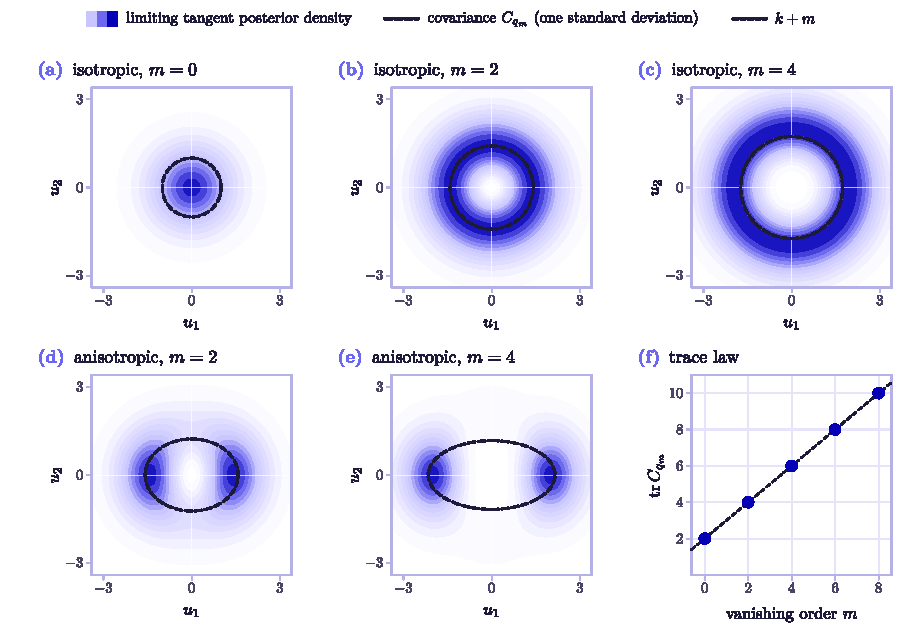
\includegraphics[width=0.923\linewidth]{figures/tilted-posterior.pdf}
  \caption{Why the vanishing order survives the small-noise rescaling, drawn in rescaled tangent coordinates with $k=2$.  Shading is the limiting tangent posterior density and the dashed curve is its covariance $C_{q_m}$.  The top row uses isotropic jets $q_m(u)=\|u\|^m$ of increasing order: at a regular point (a) the posterior is standard Gaussian and $C_{q_0}=I$, so $H_\sigma(p)$ tends to the tangent projector, while at the zeros (b) and (c) the jet hollows out the centre and the covariance inflates to $2I$ and $3I$ without changing shape.  The bottom row uses anisotropic jets at the same two orders, $q_2(u)=3u_1^2+u_2^2$ in (d) and the quartic $q_4(u)=u_1^4+0.1\,u_2^4$ of Section~\ref{sec:experiments} in (e), giving $\diag(2.5,1.5)$ and $\diag(4.636,1.364)$.  At matched order the trace is the same, $4$ in both (b) and (d) and $6$ in both (c) and (e), while the shape is not.  The order therefore fixes the trace and the jet fixes the shape, and in every panel the ellipse stays centred and nondegenerate, so the tangent range is retained throughout.  Panels (a) to (e) use equal scales on both axes, so the ellipses carry their true shape.  (f) The trace against the vanishing order for the isotropic family, with the dashed line $k+m$ of \eqref{eq:trace}; the plotted values agree with it exactly.}
  \label{fig:tilted-posterior}
\end{figure}

\paragraph{Closed forms.}
If $q_m(z)=\|z\|^m$ (with even $m$), rotational symmetry and \eqref{eq:trace} give
\begin{equation}
  C_{q_m}=\left(1+\frac{m}{k}\right)I_k.
\end{equation}
For a quadratic zero $q_2(z)=z^\top A z$, $A\succeq0$ and $A\ne0$, Isserlis' identity gives
\begin{equation}
  C_{q_2}=I_k+\frac{2A}{\tr A}.
  \label{eq:quadratic}
\end{equation}
Thus even the limiting tangent metric can be anisotropic.

\subsection{A smooth full-support counterexample}
\label{sec:counterexample}

Let $\M=S^1$, $x(\theta)=(\cos\theta,\sin\theta)$, $p=(1,0)$, and
\begin{equation}
  \rho(\theta)=\frac{1-\cos\theta}{2\pi}.
  \label{eq:circle-density}
\end{equation}
This density is $C^\infty$, nonnegative, and zero only at $p$.  Consequently, $\operatorname{supp}(\mu)=S^1$.  Since $1-\cos\theta=\theta^2/2+O(\theta^4)$, Theorem~\ref{thm:finite} yields, for the tangent vector $t=(0,1)$,
\begin{equation}
  H_\sigma(p)\longrightarrow 3tt^\top\ne tt^\top=P_{\T_pS^1}.
  \label{eq:circle-counter}
\end{equation}
Indeed, after $\theta=\sigma u$, the tangent posterior is proportional to $u^2e^{-u^2/2}$ and has variance $\E Z^4/\E Z^2=3$.  Appendix~\ref{app:examples} collects this circle family and the radial and quadratic jets.

At positive-density points, Corollary~\ref{cor:regular} recovers the usual projector limit.  The stated assumptions of Theorem~1 in arXiv v2 (28 February 2026) of \citet{kharitenko2026landing} also permit isolated zeros, because full support is weaker than pointwise positivity.\footnote{That theorem assumes ``$\M\subseteq\R^d$ a compact, embedded $C^3$-submanifold and $\mu\in\mathcal P(\R^d)$ a Borel probability measure with $\operatorname{supp}\mu=\M$ and $\mu\ll\operatorname{Vol}_\M$ such that $\tfrac{d\mu}{d\operatorname{Vol}_\M}\in C^3(\M)$'', and its Corollary~2 concludes $\lim_{\sigma\to0}\,I+\sigma^2\nabla^2\log p_\sigma(x)=P_{\T_x\M}$ for $x\in\M$.  The density \eqref{eq:circle-density} satisfies each of these hypotheses.}  The circle example shows that the conclusion requires a local positivity condition.  The local estimate in their Appendix E.2 carries $\mu(p)$ and $\mu(p)^2$ in denominators, and their Appendix E.4 supplies the missing condition by asserting that ``since $\mu(\cdot)\in C^3(\M)$ and $\operatorname{supp}\mu=\M$, there exist positive lower and upper bounds on $\mu(\cdot)$ and its derivatives on $\M$''.  With this condition, that result covers the positive-density regime, while Theorem~\ref{thm:finite} characterizes the complementary finite-type regime.

\subsection{A density-floor phase transition}
\label{sec:crossover}

Although a zero is defined pointwise, its effect persists across a noise-dependent low-density regime.  Fix a sufficiently small coordinate neighborhood $U=F_p(B(0,r_0))$.  Let an unnormalized family satisfy, for $z\in B(0,r_0)$ and $0\le\delta\le\delta_0$,
\begin{equation}
  a_\delta(z)=q_m(z)+\delta h(z)+r_\delta(z),
  \qquad h\text{ continuous},\quad h(0)=a_0>0,
\end{equation}
where $|r_\delta(z)|\le C(\|z\|^m+\delta)$ on this fixed neighborhood and
$r_\delta(z)/(\|z\|^m+\delta)\to0$ uniformly in the joint limit
$(z,\delta)\to(0,0)$.  After fixing the common local normalization, assume that the total unnormalized mass on $\M\setminus U$ is uniformly bounded as $\delta\downarrow0$.  The weaker subexponential condition $\exp(o(\sigma^{-2}))$ along $\delta=\delta_\sigma$ also suffices.  Normalization is immaterial to the posterior.  Let $\delta=\delta_\sigma\downarrow0$ with $\delta_\sigma/\sigma^m\to\lambda\in[0,\infty]$.

\begin{theorem}[Density-floor crossover]
\label{thm:crossover}
Under the local assumptions of Theorem~\ref{thm:finite}, the tangent block of $H_\sigma(p)$ converges to
\begin{equation}
  C_{q,\lambda}
  =\frac{a_0\lambda I_k+\E[ZZ^\top q_m(Z)]}
  {a_0\lambda+\E[q_m(Z)]},
  \qquad
  \tr C_{q,\lambda}
  =k+\frac{m\E[q_m(Z)]}{a_0\lambda+\E[q_m(Z)]}.
  \label{eq:crossover}
\end{equation}
For $\lambda=\infty$, the limit is $I_k$.
\end{theorem}

Appendix~\ref{app:crossovers} proves the law by rescaling the floor against the
leading jet.  Thus $\delta\ll\sigma^m$ is zero-dominated, $\delta\gg\sigma^m$ is regular-density, and $\delta\asymp\sigma^m$ interpolates nontrivially.  On the circle with $a_\delta(\theta)=\delta+1-\cos\theta$,
\begin{equation}
  \lambda=\delta/\sigma^2,\qquad
  C_{q,\lambda}=\frac{\lambda+3/2}{\lambda+1/2}.
  \label{eq:circle-crossover}
\end{equation}

There is a distinct spatial boundary layer for a \emph{fixed} distribution.  Query the denoiser at the nearby manifold point $y_\sigma=F_p(\sigma a)$, where $a\in\R^k$ is fixed, and let $\nu_{q,a}$ be the probability law with density proportional to
\begin{equation}
  q_m(u)\exp\!\left(-\tfrac12\|u-a\|^2\right).
\end{equation}
Applying the rescaling from Theorem~\ref{thm:finite} gives the following result.

\begin{proposition}[Spatial boundary layer]
\label{prop:spatial}
Under the minimal convergence assumptions of Theorem~\ref{thm:finite},
\begin{equation}
  H_\sigma(F_p(\sigma a))
  \longrightarrow U_p C_q^{\mathrm{sp}}(a)U_p^\top,
  \qquad
  C_q^{\mathrm{sp}}(a)=\Cov_{\nu_{q,a}}(u).
  \label{eq:spatial}
\end{equation}
Equivalently, if $M_q(a)=\E[q_m(a+Z)]$, then
\begin{equation}
  C_q^{\mathrm{sp}}(a)=I_k+\nabla_a^2\log M_q(a).
\end{equation}
For $k=1$ and $q_2(u)=u^2$,
\begin{equation}
  C_q^{\mathrm{sp}}(a)=\frac{a^4+3}{(a^2+1)^2}.
  \label{eq:spatial-quadratic}
\end{equation}
It equals $3$ at the zero, crosses $1$ at $|a|=1$, reaches $3/4$ at $|a|=\sqrt3$, and tends back to $1$ from below.
\end{proposition}

Appendix~\ref{app:crossovers} proves this by the same moving-query rescaling.
Under the two-order density expansion and third-order graph bound in
Theorem~\ref{thm:finite}, the same moving-query calculation gives, uniformly for $a$ in compact sets,
\begin{align}
  D_\sigma(F_p(\sigma a))-F_p(\sigma a)
  &=\sigma U_p\bigl(\E_{\nu_{q,a}}u-a\bigr)+O(\sigma^2),
  \label{eq:spatial-mean-rate}\\
  H_\sigma(F_p(\sigma a))
  &=U_pC_q^{\mathrm{sp}}(a)U_p^\top+O(\sigma).
  \label{eq:spatial-h-rate}
\end{align}
The normal component of the first line is $O(\sigma^2)$, and Davis--Kahan applied to the second line gives
$\|\mathcal P_k(H_\sigma(F_p(\sigma a)))-P_{\T_{F_p(\sigma a)}\M}\|_\op=O(\sigma)$.

The on-manifold calculation extends to normal offsets of the same scale.
Write $P=U_pU_p^\top$, $P^\perp=I-P$, and set
\begin{equation}
  \mathcal B(u)=\tfrac12\mathrm{II}_p[u,u],
  \qquad
  \mu_a=\E_{\nu_{q,a}}u,
  \qquad
  C_a=\Cov_{\nu_{q,a}}(u).
\end{equation}
Also define the normal-valued covariance and its calibrated version by
\begin{equation}
  \Gamma_a
  =\E_{\nu_{q,a}}
  \bigl[(\mathcal B(u)-\overline{\mathcal B}_a)
        (u-\mu_a)^\top\bigr],
  \qquad
  \Lambda_a=\Gamma_aC_a^{-1},
  \qquad
  \overline{\mathcal B}_a=\E_{\nu_{q,a}}\mathcal B(u).
  \label{eq:normal-boundary-objects}
\end{equation}
For $b\in\N_p\M$, let the shape operator $S_b$ and the normal map
$\mathcal B_a$ be given by
\begin{equation}
  \langle S_bv,w\rangle
  =\langle b,\mathrm{II}_p[v,w]\rangle,
  \qquad
  \mathcal B_av=\mathrm{II}_p[a,v].
  \label{eq:shape-convention}
\end{equation}

\begin{theorem}[Uniform normal-offset boundary layer]
\label{thm:normal-boundary}
Assume the two-order density expansion and third-order graph expansion of
Theorem~\ref{thm:finite}, including
$\|DR_g(z)\|_\op\le C\|z\|^2$.  Fix compact sets
$K_T\subset\R^k$ and $K_N\subset\N_p\M$.  Assume also that, for some fixed chart radius
$r$, constants $c,C>0$, and all sufficiently small $\sigma$,
\begin{equation}
  \sup_{a\in K_T,\,b\in K_N}
  \int_{\M\setminus F_p(B(0,r))}
  (1+\|x-p\|^2)
  e^{-\|x-F_p(\sigma a)-\sigma b\|^2/(2\sigma^2)}\,\mu(dx)
  \le Ce^{-c/\sigma^2}.
  \label{eq:normal-boundary-localization}
\end{equation}
This localization condition is automatic when a fixed Euclidean
neighborhood of $p$ meets $\M$ only in the chart; in particular it holds
for compact $\M$.  For the two statements below that involve nearest-point projection we assume in addition that $\M$ has positive reach and that $\sigma$ is small enough for
$\mathcal V_\sigma(K_T,K_N)$ to lie within a tubular neighborhood of radius
smaller than that reach, so $\pi$ is single valued on it; the expansions of
$D_\sigma$, $H_\sigma$, and $Q_\sigma$ do not use $\pi$.  Let
\begin{equation}
  \mathcal V_\sigma(K_T,K_N)
  =\{F_p(\sigma a)+\sigma b:a\in K_T,\ b\in K_N\}.
  \label{eq:normal-boundary-set}
\end{equation}
Then, uniformly for $a\in K_T$ and $b\in K_N$,
\begin{align}
  D_\sigma(y)-y
  &=\sigma\{U_p(\mu_a-a)-b\}+O(\sigma^2),
  \label{eq:normal-boundary-mean}\\
  U_p^\top H_\sigma(y)U_p
  &=C_a+O(\sigma),\nonumber\\
  P^\perp H_\sigma(y)U_p
  &=\sigma\Gamma_a+O(\sigma^2),\qquad
  P^\perp H_\sigma(y)P^\perp
  =\sigma^2\Cov_{\nu_{q,a}}(\mathcal B(u))+O(\sigma^3).
  \label{eq:normal-boundary-blocks}
\end{align}
In particular, if $c_0=\inf_{a\in K_T}\lambda_{\min}(C_a)>0$ and
$Q_\sigma(y)=\mathcal P_k(H_\sigma(y))$, then, for all sufficiently small
$\sigma$,
\begin{align}
  \lambda_k(H_\sigma(y))&\ge c_0-O(\sigma),&
  \lambda_{k+1}(H_\sigma(y))&=O(\sigma^2),
  \label{eq:normal-boundary-gap}\\
  Q_\sigma(y)
  &=P+\sigma\{\Lambda_aU_p^\top+U_p\Lambda_a^\top\}
    +O(\sigma^2).
  \label{eq:normal-boundary-projector}
\end{align}
Moreover, nearest projection and population normal-only landing obey
\begin{align}
  \pi(y)
  &=F_p\!\left(\sigma a+\sigma^2S_ba+O(\sigma^3)\right),
  \label{eq:normal-boundary-projection}\\
  \overline D_{\sigma,Q_\sigma}(y)-\pi(y)
  &=\sigma^2\Bigl[
      U_p\{\Lambda_a^\top b-S_ba\}
      +\overline{\mathcal B}_a-\mathcal B(a)
      -\Lambda_a(\mu_a-a)
    \Bigr]+O(\sigma^3),
  \label{eq:normal-boundary-landing}
\end{align}
where
$\overline D_{\sigma,Q}(y)=y+(I-Q(y))(D_\sigma(y)-y)$.
All remainders are uniform on $K_T\times K_N$.

Finally, let
$W_{F_p(z)}=DF_p(z)(DF_p(z)^\top DF_p(z))^{-1/2}$ and set
$A_{0,\sigma}(y)=W_{\pi(y)}C_aW_{\pi(y)}^\top$.  Then
$\range(A_{0,\sigma}(y))=\T_{\pi(y)}\M$ and, on
$\mathcal V_\sigma(K_T,K_N)$,
\begin{equation}
  \beta_H(\sigma)=O(\sigma),\qquad
  \beta_L(\sigma)=O(\sigma^2),\qquad
  g_\sigma\ge c_0/2,\qquad
  \sup_y\|D_\sigma(y)-y\|=O(\sigma),
  \label{eq:normal-boundary-rates}
\end{equation}
in the notation of Corollary~\ref{cor:learned}, where $\beta_H$ is the
supremum over the query set of $\|H_\sigma-A_{0,\sigma}\|_\op$, that is the
population bias of the link Hessian against the reference field just defined,
$\beta_L$ is the corresponding supremum of the normal-only landing error
$\|\overline D_{\sigma,Q_\sigma}-\pi\|$, and $g_\sigma$ is the infimum of the
tangent-normal eigengap $\lambda_k(H_\sigma)-\lambda_{k+1}(H_\sigma)$.
\end{theorem}

Appendix~\ref{app:normal-boundary} proves it.  The theorem concerns a shrinking $O(\sigma)$ tube, the scale needed for the
uniform population bounds used in local optimization.  On a fixed-width
tube, Lemma~\ref{lem:landing-decomposition} shows why the same
$O(\sigma^2)$ landing rate generally fails.

Because $C_{q,\lambda}$ is a scalar convex combination of $C_q$ and $I_k$, each eigenvalue moves monotonically toward one as the floor grows.  The matrix path need not be monotone in Loewner order.  The spatial law need not be eigenvalue-monotone either, because shifting the Gaussian window changes both the posterior mean and variance.  The experiments therefore treat the two mechanisms separately.

\begin{takeawaybox}[Two nearby regimes]
A positive density floor does not restore regular-density geometry until it is resolved at the noise scale: floors $\delta=o(\sigma^m)$ retain the finite-zero limiting spectrum.  With the density fixed, queries within $O(\sigma)$ of the zero instead follow the spatial boundary-layer law.  The two transitions arise from different perturbations.
\end{takeawaybox}

\section{Spectral calibration}
\label{sec:calibration}

Let $A_0=UC_qU^\top$ and $c_q=\lambda_{\min}(C_q)>0$.  Given a symmetric estimate $\widehat A$, define the hard calibration
\begin{equation}
  \mathcal{P}_k(\widehat A)
  :=\text{orthogonal projector onto the top-$k$ eigenspace of }\widehat A.
  \label{eq:hard}
\end{equation}
If $k$ is unknown, it can be selected by thresholding inside the tangent-normal spectral gap under the condition stated below.  For a differentiable score network $s_\theta$, the input is the symmetrized link Jacobian
\begin{equation}
  \widehat A_\theta(y)=\tfrac12\bigl(A_\theta(y)+A_\theta(y)^\top\bigr),
  \qquad A_\theta(y)=I_d+\sigma^2\nabla s_\theta(y).
\end{equation}

\begin{proposition}[Stable hard calibration]
\label{prop:hard}
If $\|\widehat A-A_0\|_\op\le\eta<c_q/2$, then
\begin{equation}
  \|\mathcal{P}_k(\widehat A)-UU^\top\|_\op
  \le \frac{2\eta}{c_q}.
  \label{eq:hard-bound}
\end{equation}
Write $P=UU^\top$ and $P^\perp=I_d-P$, and let $U_\perp$ have orthonormal columns
spanning $\range(U)^\perp$, so that its columns form a basis of the normal
space.  Set
\begin{equation}
  \delta(\widehat A)
  :=\lambda_{\min}\bigl(U^\top\widehat AU\bigr)
   -\lambda_{\max}\bigl(U_\perp^\top\widehat AU_\perp\bigr).
  \label{eq:computed-separation}
\end{equation}
Whenever $\delta(\widehat A)>0$, without any hypothesis on $\eta$,
\begin{equation}
  \|\mathcal{P}_k(\widehat A)-UU^\top\|_\op
  \le\frac{\|P^\perp\widehat AP\|_\op}{\delta(\widehat A)},
  \label{eq:hard-residual}
\end{equation}
in which only the tangent-normal coupling block of the error appears: since
$P^\perp A_0P=0$, we have $P^\perp\widehat AP=P^\perp(\widehat A-A_0)P$.  In
particular an error confined to the tangent block leaves
$\mathcal P_k(\widehat A)=UU^\top$ exactly, however large its eigenvalue bias.
Under the standing hypothesis $\eta<c_q/2$, Weyl's inequality gives
$\delta(\widehat A)\ge c_q-2\eta>0$, so \eqref{eq:hard-residual} is then
available with a denominator depending only on $c_q$ and $\eta$.  Both blocks in
\eqref{eq:computed-separation} are computable from $\widehat A$ and a tangent
frame, so \eqref{eq:hard-residual} remains informative in regimes where
$\eta<c_q/2$ fails.
For every threshold $\vartheta_{\mathrm{sp}}\in(\eta,c_q-\eta)$,
$\mathbf 1_{(\vartheta_{\mathrm{sp}},\infty)}(\widehat A)$ has rank $k$ and equals
$\mathcal P_k(\widehat A)$; thus the same condition gives unknown-$k$ rank recovery.
In addition,
\begin{equation}
  \left|\sum_{i=1}^k\lambda_i(\widehat A)-(k+m)\right|\le k\eta;
\end{equation}
hence $m=\operatorname{round}(\sum_{i=1}^k\lambda_i(\widehat A)-k)$ whenever $k\eta<1/2$.
\end{proposition}

A soft alternative is obtained after projecting $\widehat A$ onto the positive-semidefinite cone:
\begin{equation}
  \Phi_\tau(\widehat A_+)=\widehat A_+(\widehat A_++\tau I)^{-1}.
  \label{eq:soft}
\end{equation}

\begin{proposition}[Stable soft calibration]
\label{prop:soft}
If $\widehat A\succeq0$ and $\|\widehat A-A_0\|_\op\le\eta$, then for every $\tau>0$,
\begin{equation}
  \|\Phi_\tau(\widehat A)-UU^\top\|_\op
  \le \frac{\tau}{c_q}+\frac{\eta}{\tau}.
  \label{eq:soft-bound}
\end{equation}
Balancing the two terms gives an $O(\sqrt{\eta/c_q})$ error without forming a hard top-$k$ eigenspace.
\end{proposition}

Appendix~\ref{app:spectral} proves the hard bound with Davis--Kahan and the soft bound with the resolvent identity.  If the estimator is PSD by construction, the rational filter avoids a hard eigenspace cutoff.  A general symmetric score Jacobian may still require an eigendecomposition to form $\widehat A_+$.  The estimate $\|\widehat A-A_0\|_\op\le\eta$ yields $\|\widehat A_+-A_0\|_\op\le2\eta$, so for a symmetric estimate that is not positive semidefinite the composed form of Proposition~\ref{prop:soft} reads $\|\Phi_\tau(\widehat A_+)-UU^\top\|_\op\le\tau/c_q+2\eta/\tau$, which balances at $2\sqrt{2\eta/c_q}$.  The raw operator $A_0$ remains a positive-definite preconditioner on the tangent space and therefore preserves first-order stationary points.  Calibration removes density-dependent conditioning and gives the step size the same interpretation as in Riemannian gradient descent.  The optimization results below use the hard rank-$k$ orthogonal projector.  We evaluate the soft contraction in \eqref{eq:soft} only as a geometric estimator.  The experiments assume known $k$, apart from a separately reported threshold-at-$1/2$ rank diagnostic.  The present guarantees do not cover adaptive threshold selection.  That diagnostic is licensed only when $c_q>1/2+\eta$, and $c_q$ is not bounded below by $1/2$ uniformly in the vanishing order.  For $k=2$, minimizing $\lambda_{\min}(C_q)$ numerically over the nonnegative binary forms $q(z)=\prod_j(z_1-t_jz_2)^2$ gives $0.879$, $0.670$, $0.534$, $0.442$, $0.380$, and $0.333$ at orders $m=4,8,12,16,20,24$.  The diagnostic is therefore sound at the orders used in Section~\ref{sec:experiments} but fails for deep zeros: at $m=16$ a threshold of $1/2$ discards a genuine tangent direction even when the operator is exact.  Lemma~\ref{lem:universal-gap} guarantees a positive constant depending on $k$ and $m$, not a constant exceeding $1/2$.

\section{Density-calibrated optimization}
\label{sec:optimization}

Calibrating only the gradient multiplier is insufficient if a raw denoiser is subsequently used as the landing map.  We avoid the word retraction for $\overline D_Q$, which does not map into $\M$ and does not fix manifold points at positive $\sigma$, so it is not a retraction in the sense of \citet{absil2008optimization}; the analysis never uses those axioms, only the landing error in \eqref{eq:oracle-errors}.  At a symmetric finite-type center,
$D_\sigma(p)=p+O(\sigma^2)$ and $H_\sigma(p)\to U C_qU^\top$.  For a locally isotropic quadratic objective centered at $p$, the tangent linearization of
\begin{equation}
  x\longmapsto D_\sigma\!\left(x-\gamma H_\sigma(x)\nabla f(x)\right)
  \label{eq:raw-drgd}
\end{equation}
converges to $C_q(I-\gamma C_q)$.  Replacing the inner $H_\sigma$ by $P_{\T_p\M}$ still leaves the limiting factor $C_q(I-\gamma I)$: the outer denoiser reintroduces density-dependent expansion.

Normal-only landing avoids this effect.  Given $Q(y)$, define
\begin{equation}
  \overline D_Q(y):=y+(I-Q(y))(D(y)-y).
  \label{eq:normal-landing}
\end{equation}
For the population denoiser of a distribution supported on an affine manifold, exact $Q=P_{\T_p\M}$ makes this map the exact orthogonal projection for every $\sigma$ and leaves tangent coordinates unchanged.  On a curved manifold, it is an inexact landing map.  The next result treats that error abstractly.  Throughout this section, $\M$ is compact, $C^3$, and has positive reach, and $\pi$ denotes nearest-point projection in a reach tube $\mathcal{T}_r=\{x:\dist(x,\M)<r\}$.

The spatial law quantifies the difference.  For a one-dimensional quadratic zero and $y_\sigma=F_p(\sigma a)$,
\begin{equation}
  D_\sigma(y_\sigma)-y_\sigma
  =\sigma U_p\frac{2a}{a^2+1}+O(\sigma^2).
  \label{eq:tangent-drift}
\end{equation}
Thus raw denoising has an $O(\sigma)$ tangent drift throughout the boundary layer, pointing away from the zero.  Exact normal-only landing removes that term and leaves an $O(\sigma^2)$ curvature residual.

\begin{lemma}[Normal-only landing decomposition]
\label{lem:landing-decomposition}
Let $p=\pi(y)$, $v=y-p\in\N_p\M$, $r_D=D(y)-p$, and let $Q(y)$ be an orthogonal projector satisfying
$\|Q(y)-P_{\T_p\M}\|_\op\le\eps_P$.  Then
\begin{equation}
  \overline D_Q(y)-p=Q(y)v+(I-Q(y))r_D,
  \label{eq:landing-decomposition}
\end{equation}
and therefore
\begin{equation}
  \|\overline D_Q(y)-\pi(y)\|
  \le \eps_P\dist(y,\M)
  +\eps_P\|P_{\T_p\M}r_D\|
  +\|(I-P_{\T_p\M})r_D\|.
  \label{eq:landing-decomposition-bound}
\end{equation}
\end{lemma}

The first term cannot be omitted.  Under the stronger moving-query expansion \eqref{eq:spatial-mean-rate}--\eqref{eq:spatial-h-rate}, an on-manifold spatial boundary layer has $\eps_P=O(\sigma)$, an $O(\sigma)$ tangent component of $r_D$, and an $O(\sigma^2)$ normal component.  Equation~\eqref{eq:landing-decomposition-bound} then gives an $O(\sigma^2)$ error.  On a fixed-width tube, the same bound permits only an $O(\sigma)$ guarantee because projector tilt can act on an $O(1)$ normal displacement.  Appendix~\ref{app:optimization} proves the lemma and details this distinction.

\begin{assumption}[Inexact normal landing and tangent oracles]
\label{ass:oracles}
Let $\mathcal V\subseteq\mathcal{T}_r$ be a set containing every iterate $x_t$ and every intermediate point $z_t$ of the recursion below.  On $\mathcal V$, a landing map $L$ and rank-$k$ orthogonal projector $Q$ satisfy
\begin{equation}
  \|L(z)-\pi(z)\|\le\eps_L,
  \qquad
  \|Q(x)-P_{\T_{\pi(x)}\M}\|_\op\le\eps_P.
  \label{eq:oracle-errors}
\end{equation}
The intended construction is $L=\overline D_Q$ from \eqref{eq:normal-landing}; the theorem also applies to an independently learned landing map satisfying the displayed error.  We state the hypothesis on $\mathcal V$ rather than on all of $\mathcal T_r$ because the proof invokes these inequalities only at the visited points, and because the rates available from Theorem~\ref{thm:normal-boundary} are established on an $O(\sigma)$ layer rather than on a tube of fixed width.  Taking $\mathcal V=\mathcal T_r$ is admissible whenever uniform bounds of this form are available there.
\end{assumption}

For an ambient differentiable objective $f$, define spectrally calibrated denoising Riemannian gradient descent (SC-DRGD):
\begin{equation}
  z_t=x_t-\gamma Q(x_t)\nabla f(x_t),
  \qquad x_{t+1}=L(z_t).
  \label{eq:scdrgd}
\end{equation}
In practice $D=D_\theta$, $Q=\mathcal{P}_k(\widehat A_\theta)$, and $L=\overline D_{\theta,Q}$.  Evaluation-point and estimation differences are absorbed into \eqref{eq:oracle-errors}.

\begin{theorem}[Inexact SC-DRGD]
\label{thm:optimization}
Suppose $f$ has $L_f$-Lipschitz gradient and $\|\nabla f\|\le B$ on $\mathcal{T}_r$.  Let $F=f\circ\pi$ have $L_F$-Lipschitz gradient there, let $\pi$ be $L_\pi$-Lipschitz, and assume
\begin{equation}
  \|\mathrm d\pi_x-P_{\T_{\pi(x)}\M}\|_\op
  \le K_\pi\dist(x,\M).
\end{equation}
Let $L$ and $Q$ satisfy Assumption~\ref{ass:oracles} on a set $\mathcal V$ containing every $x_t$ and $z_t$.  Initialize $\dist(x_0,\M)\le\eps_L$, which one landing step from any $x_{-1}\in\mathcal T_{r-\gamma B}$ achieves.  If
\begin{equation}
  \gamma B+\eps_L<r,
  \qquad L_\pi\eps_L<r,
  \qquad 0<\gamma\le(4L_F)^{-1},
\end{equation}
then every $x_t$ is $\eps_L$-feasible and, with
\begin{equation}
  e=(K_\pi B+L_f)\eps_L+B\eps_P,
  \label{eq:eopt}
\end{equation}
we have for $p_t=\pi(x_t)$
\begin{equation}
  \frac1N\sum_{t=0}^{N-1}\|\grad_\M f(p_t)\|^2
  \le
  \frac{4(F(x_0)-\inf_\M f)}{\gamma N}
  +9e^2+\frac{4BL_\pi\eps_L}{\gamma}.
  \label{eq:opt-bound}
\end{equation}
\end{theorem}

The term $4BL_\pi\eps_L/\gamma$ in \eqref{eq:opt-bound} is the accumulated objective drift caused by landing error at successive iterations.  The tangent-projector error appears through the quadratic term $e^2$.  Appendix~\ref{app:optimization} gives the perturbed descent argument for $F=f\circ\pi$.

\begin{corollary}[Learned-score reduction to population biases]
\label{cor:learned}
Let $\mathcal V\subset\mathcal T_r$ contain every tangent-step query $x_t$ and landing query $z_t$ of the run under consideration.  For each $y\in\mathcal V$, suppose a PSD rank-$k$ field $A_{0,\sigma}(y)$ satisfies
\begin{equation}
  \range(A_{0,\sigma}(y))=\T_{\pi(y)}\M,
  \qquad \lambda_k(A_{0,\sigma}(y))\ge c>0.
\end{equation}
Define $Q_\sigma=\mathcal P_k(H_\sigma)$ and the population quantities
\begin{align}
  \beta_H(\sigma)&=\sup_{y\in\mathcal V}
  \|H_\sigma(y)-A_{0,\sigma}(y)\|_\op,\\
  \beta_L(\sigma)&=\sup_{y\in\mathcal V}
  \|\overline D_{\sigma,Q_\sigma}(y)-\pi(y)\|,\\
  g_\sigma&=\inf_{y\in\mathcal V}
  \{\lambda_k(H_\sigma(y))-\lambda_{k+1}(H_\sigma(y))\}.
\end{align}
Assume $g_\sigma>0$, $\sup_{\mathcal V}\|D_\sigma(y)-y\|\le R_D$, and a learned score satisfies uniformly on $\mathcal V$
\begin{equation}
  \|s_\theta-s_\sigma\|\le\eps_s,
  \qquad
  \|\nabla s_\theta-\nabla s_\sigma\|_\op\le\eps_J.
\end{equation}
Set $D_\theta(y)=y+\sigma^2s_\theta(y)$,
$\widehat A_\theta=\operatorname{sym}(I+\sigma^2\nabla s_\theta)$, and $Q_\theta=\mathcal P_k(\widehat A_\theta)$.  If
\begin{equation}
  \beta_H(\sigma)+\sigma^2\eps_J<c/2,
  \qquad \sigma^2\eps_J<g_\sigma/2,
\end{equation}
then the two oracle inequalities in \eqref{eq:oracle-errors} hold on $\mathcal V$ for the learned normal-only landing and projector, with
\begin{align}
  \eps_P&\le \frac{2(\beta_H(\sigma)+\sigma^2\eps_J)}{c},\label{eq:learned-projector}\\
  \eps_L&\le\beta_L(\sigma)+\sigma^2\eps_s
  +\frac{2R_D\sigma^2\eps_J}{g_\sigma}.
  \label{eq:learned-landing-main}
\end{align}
\end{corollary}

Appendix~\ref{app:optimization} derives both oracle errors from the uniform score
bounds.  Provided $\mathcal V$ contains every $x_t$ and $z_t$ used in the descent proof, Corollary~\ref{cor:learned} supplies the two oracle bounds required by Theorem~\ref{thm:optimization}; that theorem's remaining hypotheses are unchanged.  Evaluated at the finite-type center alone, with
$A_{0,\sigma}=U_pC_{q_m}U_p^\top$, Theorem~\ref{thm:finite} gives
$\beta_H=O(\sigma^2)$; this is a pointwise consistency check rather than a
visited set, since a nonstationary run does not remain at $p$.
Theorem~\ref{thm:normal-boundary} supplies
$\beta_H=O(\sigma)$, $\beta_L=O(\sigma^2)$, and $g_\sigma=\Omega(1)$
uniformly on an $O(\sigma)$ boundary layer.  If
$\eps_s,\eps_J=O(1)$ and $\gamma$ is fixed independently of $\sigma$, then
$\eps_P=O(\sigma)$ and $\eps_L=O(\sigma^2)$, and after the
$O((\gamma N)^{-1})$ transient in \eqref{eq:opt-bound} the residual bound on
the averaged squared stationarity measure is $O(\sigma^2)$.

This last instantiation carries a consistency requirement that we state
explicitly.  One step of Theorem~\ref{thm:optimization} moves $x_t$ by
$\gamma\|h_t\|$, which is $\Theta(\gamma)$ wherever $\|\nabla f\|$ is bounded
away from zero, whereas the layer of Theorem~\ref{thm:normal-boundary} has
ambient radius $O(\sigma)$.  For a $\sigma$-independent step size the visited
set therefore stays inside that layer only when the run is already ambient-near-stationary, $\|\nabla f(x_t)\|=O(\sigma/\gamma)$ throughout;
Corollary~\ref{cor:local-invariant} establishes precisely that configuration and
gives a stronger conclusion there.  Away from it, Theorem~\ref{thm:optimization}
remains valid with whatever $\beta_H$, $\beta_L$, and $g_\sigma$ hold uniformly
on the actual visited set.  Obtaining these on a macroscopic region requires a
positive density lower bound away from the zero, in the manner of the
positive-density analyses cited in Section~\ref{sec:related}; we do not prove
such a uniform statement here.  On a fixed-width
tube, Lemma~\ref{lem:landing-decomposition} permits only
$\eps_L=O(\sigma)$ in general, and hence only an $O(\sigma)$ residual for fixed
$\gamma$.  Statistical guarantees converting an $L^2$ denoising loss into
the local uniform errors above remain open.

\begin{corollary}[Local invariant SC-DRGD basin]
\label{cor:local-invariant}
Assume Theorem~\ref{thm:normal-boundary} on
\begin{equation}
  \mathcal V_\sigma^+
  =\mathcal V_\sigma
  \bigl(\overline B(0,R_+),
        \{b\in\N_p\M:\|b\|\le B_+\}\bigr)
  \label{eq:local-query-set}
\end{equation}
for fixed $R_+,B_+>0$.  Let $f$ be $C^3$ near $p$ and suppose
\begin{equation}
  \nabla f(p)=0,\qquad
  G_f=U_p^\top\nabla^2f(p)U_p\succ0.
  \label{eq:local-objective}
\end{equation}
Fix a \emph{$\sigma$-independent} step size $\gamma$ such that
\begin{equation}
  \rho=\|I_k-\gamma G_f\|_\op<1;
  \qquad\text{equivalently,}\qquad
  0<\gamma<2/\lambda_{\max}(G_f).
  \label{eq:local-contraction}
\end{equation}
Let $\widehat D_\sigma$ and symmetric $\widehat H_\sigma$ be defined on
$\mathcal V_\sigma^+$ and satisfy
\begin{align}
  \delta_D(\sigma)
  &=\sup_{\mathcal V_\sigma^+}
    \|\widehat D_\sigma-D_\sigma\|,\nonumber\\
  \delta_H(\sigma)
  &=\sup_{\mathcal V_\sigma^+}
    \|\widehat H_\sigma-H_\sigma\|_\op,\qquad
  \omega_\sigma
  =\sigma+\delta_H(\sigma)+\frac{\delta_D(\sigma)}{\sigma}
  \longrightarrow0.
  \label{eq:local-errors}
\end{align}
Define
\begin{equation}
  \widehat Q_\sigma=\mathcal P_k(\widehat H_\sigma),
  \qquad
  \widehat L_\sigma(y)
  =y+(I-\widehat Q_\sigma(y))
       (\widehat D_\sigma(y)-y).
  \label{eq:local-learned-oracles}
\end{equation}
Choose $0<R_0<R<R_+$ and initialize
\begin{equation}
  x_0=F_p(\sigma a_0)+\sigma b_0,\qquad
  \|a_0\|\le R_0,\qquad
  \|b_0\|\le M_0\omega_\sigma
  \label{eq:local-initialization}
\end{equation}
for fixed $M_0$.  Then, for all sufficiently small $\sigma$, the iterates
\begin{equation}
  z_t=x_t-\gamma\widehat Q_\sigma(x_t)\nabla f(x_t),
  \qquad
  x_{t+1}=\widehat L_\sigma(z_t)
  \label{eq:local-scdrgd}
\end{equation}
remain in $\mathcal V_\sigma^+$ for every $t$.  They have unique
fixed-chart coordinates
$x_t=F_p(\sigma a_t)+\sigma b_t$, $b_t\in\N_p\M$, satisfying, for
constants $C,M$ independent of $t$ and $\sigma$,
\begin{align}
  a_{t+1}
  &=(I_k-\gamma G_f)a_t+e_t,
  &\|e_t\|&\le C\omega_\sigma,
  \label{eq:local-recurrence}\\
  \|a_t\|
  &\le\rho^t\|a_0\|
    +\frac{C}{1-\rho}\omega_\sigma,
  &\|b_t\|&\le M\omega_\sigma.
  \label{eq:local-coordinate-bounds}
\end{align}
In particular, with $p_t=\pi(x_t)$,
\begin{align}
  \dist(x_t,\M)
  &\le C\sigma\omega_\sigma,\label{eq:local-feasibility}\\
  \|x_t-p\|+\|\grad_\M f(p_t)\|
  &\le
  C\sigma\left(
    \rho^t\|a_0\|+\frac{\omega_\sigma}{1-\rho}
  \right).
  \label{eq:local-stationarity}
\end{align}
\end{corollary}

Appendix~\ref{app:local-invariant} proves the basin is invariant.  For population
oracles, $\omega_\sigma=\sigma$, so the asymptotic
feasibility and stationarity floors are $O(\sigma^2)$.  If
$\widehat D_\sigma=y+\sigma^2s_\theta$ and
$\widehat H_\sigma=\operatorname{sym}(I+\sigma^2\nabla s_\theta)$, then
$\delta_D\le\sigma^2\eps_s$ and $\delta_H\le\sigma^2\eps_J$.  Bounded
$\eps_s,\eps_J$ preserve the same $O(\sigma^2)$ floors.  The conclusion is local.  Appendix~\ref{app:normal-gradient-caveat} explains why that hypothesis is needed.  It establishes the visited-set condition near an ambient stationary point with positive-definite tangent Hessian, but does not show that an arbitrary trajectory enters or remains in a finite-type boundary layer.

\begin{takeawaybox}[Both steps matter]
Calibrating the tangent update alone does not remove density-dependent scaling from the full update.  Normal-only landing removes the raw denoiser's tangent displacement; without it, the outer derivative restores the scaling removed from the inner step.
\end{takeawaybox}

\section{Population, finite-sample, and learned-score evidence}
\label{sec:experiments}

The experiments separate population, finite-sample, and learned-model effects.  Deterministic quadrature evaluates population posterior moments, empirical posterior estimation adds finite-sample error, and the learned-model studies add model and Jacobian error, first in geometric estimation and then inside an optimizer.  Appendix~\ref{app:experiments} records the protocol, seeds and numerical self-checks.

\subsection{Spectral law on the circle}

We begin with deterministic quadrature, which removes sampling and learning error.  For $r\in\{0,1,2,4\}$, let $\rho_r(\theta)\propto(1-\cos\theta)^r$ and evaluate $H_\sigma(p)$ at $p=(1,0)$.  Here the vanishing order is $m=2r$, so Theorem~\ref{thm:finite} predicts tangent eigenvalue $1+2r$ and normal eigenvalue zero.  Figure~\ref{fig:circle-spectrum} approaches $1,3,5,$ and $9$ without fitted constants.

\begin{figure}[!htbp]
  \centering
  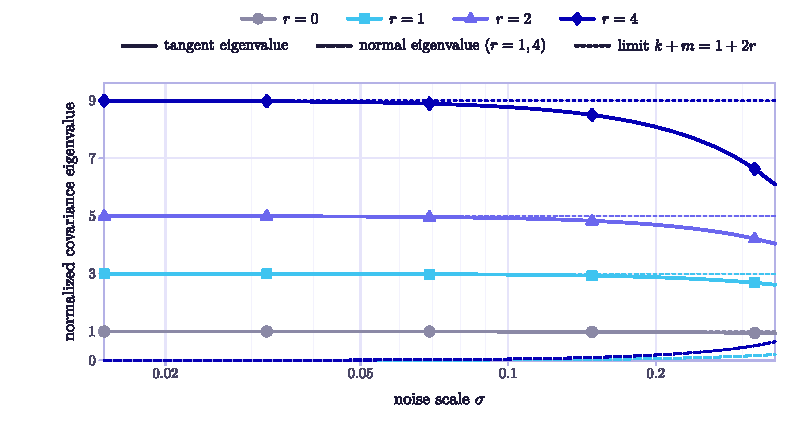
\includegraphics[width=0.821\linewidth]{figures/circle-spectrum.pdf}
  \caption{Population posterior-covariance spectra on $S^1$, computed by deterministic quadrature.  Solid curves are tangent eigenvalues for density zeros of order $m=2r$; dashed curves show representative normal eigenvalues.  The small-noise limits are the theorem's $k+m=1+2r$.  The horizontal axis is the noise scale on a logarithmic scale, and the vertical axis is the normalized covariance eigenvalue.}
  \label{fig:circle-spectrum}
\end{figure}

\subsection{Finite-sample range and order recovery}

We draw samples from the same quadratic-zero circle and form the exact empirical Gaussian-KDE posterior
\begin{equation}
  \widehat D_N=\frac{\sum_iw_iX_i}{\sum_iw_i},
  \qquad
  \widehat H_N=
  \frac{\sum_iw_i(X_i-\widehat D_N)(X_i-\widehat D_N)^\top}
  {\sigma^2\sum_iw_i},
  \quad
  w_i=e^{-\|X_i-p\|^2/(2\sigma^2)}.
  \label{eq:empirical-kde}
\end{equation}
Population asymptotics do not indicate how estimation quality changes with realized local sample coverage.  Figure~\ref{fig:kde} addresses this question with $48$ independently seeded replications, $N\in\{20{,}000,80{,}000,320{,}000\}$, and five fixed noise levels.  In panel (a), both $\widehat H_N$ and its top-one projector are compared with finite-noise population references from deterministic quadrature, so deterministic finite-$\sigma$ bias is not counted as sampling error.  The horizontal coordinate is the realized effective sample size $(\sum_iw_i)^2/\sum_iw_i^2$.  Panel (b) asks a harder question: how often does $\operatorname{round}(\lambda_1(\widehat H_N)-1)$ recover the true order $m=2$?  In this symmetric one-dimensional setting, the projector is already accurate at low effective sample size, whereas rounded-order recovery improves only with greater local coverage.  We report this as a descriptive sweep, not as a concentration result.

\begin{figure}[!htbp]
  \centering
  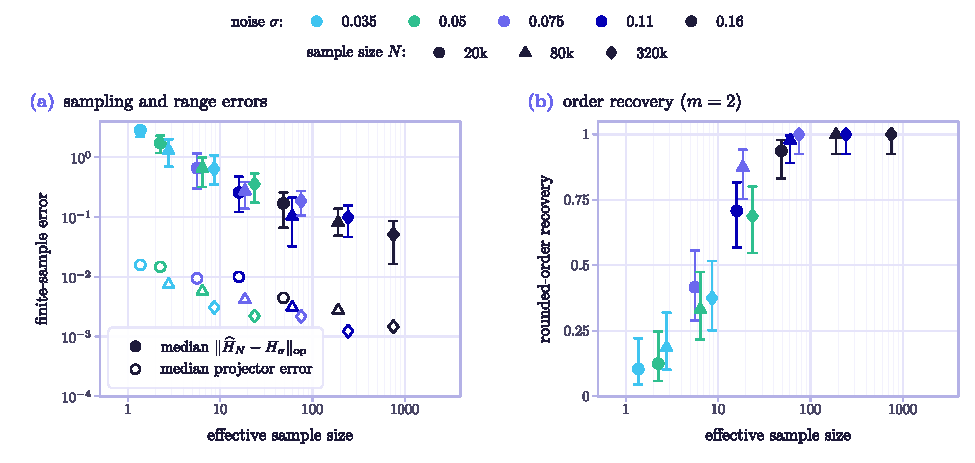
\includegraphics[width=\linewidth]{figures/finite-sample-kde.pdf}
  \caption{Finite-sample empirical-posterior experiment.  Each point summarizes $48$ replications.  Color denotes $\sigma$, while circles, triangles, and diamonds denote $N=20\mathrm{k},80\mathrm{k},320\mathrm{k}$.  (a) Filled points and bars are medians and interquartile ranges of $\|\widehat H_N-H_\sigma\|_\op$; open points are median top-one projector errors, both relative to finite-noise population references computed by deterministic quadrature.  (b) Fraction recovering $m=2$ after rounding $\lambda_1(\widehat H_N)-1$, with Wilson $95\%$ binomial intervals.  Both panels use a logarithmic horizontal axis giving the effective sample size; the left vertical axis is the finite-sample operator-norm error on a logarithmic scale, and the right vertical axis is the fraction of replications recovering the rounded order, on a linear scale.}
  \label{fig:kde}
\end{figure}

\subsection{Near-zero crossover}

With $\rho_\delta(\theta)\propto\delta+1-\cos\theta$, Figure~\ref{fig:crossover} plots the tangent eigenvalue against $\delta/\sigma^2$.  Results from four noise levels collapse onto the parameter-free prediction \eqref{eq:circle-crossover}.  The experiment shows when a strictly positive density floor changes the score geometry at the current noise scale: the curves are organized by whether $\rho(p)$ is resolved at that scale, not by the binary distinction $\rho(p)=0$ versus $\rho(p)>0$.

\begin{figure}[!htbp]
  \centering
  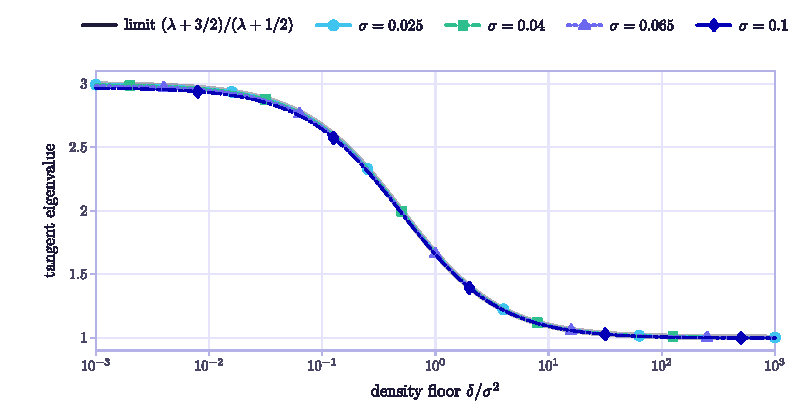
\includegraphics[width=0.821\linewidth]{figures/crossover.pdf}
  \caption{Density-floor crossover.  Deterministic quadrature at four noise levels collapses onto $(\lambda+3/2)/(\lambda+1/2)$, interpolating between the finite-zero value $3$ and regular-density value $1$.  The horizontal axis is the density floor divided by $\sigma^2$ on a logarithmic scale, and the vertical axis is the tangent eigenvalue.}
  \label{fig:crossover}
\end{figure}

\subsection{Spatial boundary layer}

To separate query displacement from the density-floor effect, we now hold the distribution fixed at $\rho(\theta)\propto1-\cos\theta$ and query at angle $\theta_\sigma=\sigma a$ from its zero.  The tangent-normal cross block need not vanish at finite $\sigma$, so Figure~\ref{fig:spatial} reports the tangent block rather than labeling it an exact eigenvalue.  It converges to the limit of Proposition~\ref{prop:spatial}, recorded in \eqref{eq:spatial-quadratic}, but not monotonically: the quotient can fall below the regular value $1$ before returning to it.  This behavior comes from moving the Gaussian window through one distribution, rather than changing the distribution through a density floor.  Both this experiment and the landing measurement below query on the manifold.  Theorem~\ref{thm:normal-boundary} also covers queries displaced along the normal, and Table~\ref{tab:normal-offset} checks that case separately: the tangent block is $C_a+O(\sigma)$ with a limit independent of the normal coordinate, while the landing bias is $O(\sigma^2)$ with a limit that depends on it.

\begin{figure}[!htbp]
  \centering
  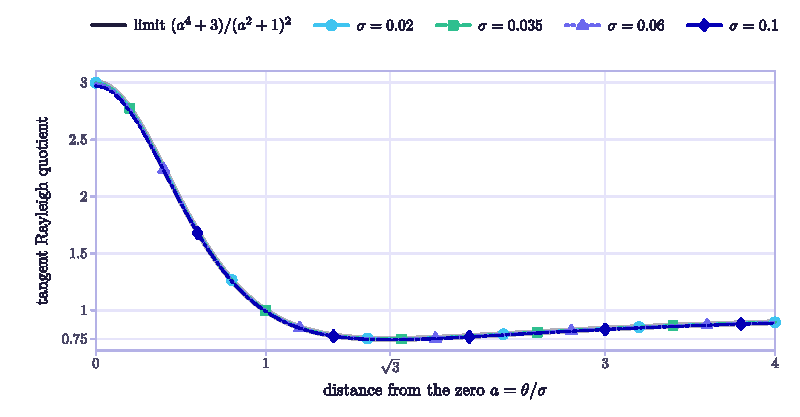
\includegraphics[width=0.821\linewidth]{figures/spatial-boundary-layer.pdf}
  \caption{Spatial boundary layer around a fixed quadratic zero.  Population circle tangent Rayleigh quotients computed by deterministic quadrature at four noise levels converge to $(a^4+3)/(a^2+1)^2$.  The nonmonotone undershoot is distinct from the monotone density-floor crossover in Figure~\ref{fig:crossover}.  The horizontal axis is the query distance from the zero divided by the noise, and the vertical axis is the tangent Rayleigh quotient; both are linear.}
  \label{fig:spatial}
\end{figure}

\subsection{Raw versus normal-only landing}

In the same fixed-distribution boundary layer, Figure~\ref{fig:landing-error} measures the denoiser's value error.  After division by $\sigma$, its raw tangent component converges to $2a/(a^2+1)$, which rules out a uniform $O(\sigma^2)$ retraction approximation there.  Projecting the denoising displacement into the normal space removes that entire tangent term; the remaining error collapses after division by $\sigma^2$.

\begin{figure}[!htbp]
  \centering
  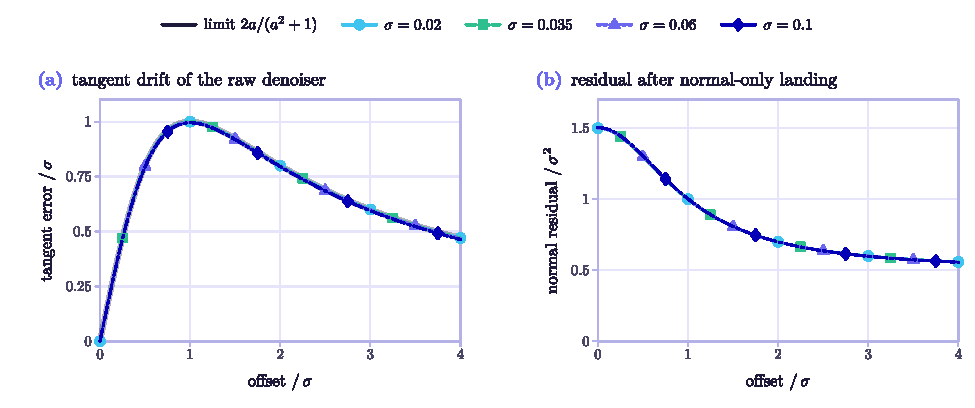
\includegraphics[width=\linewidth]{figures/landing-error.pdf}
  \caption{Effect of normal-only landing.  Left: the raw denoiser has an $O(\sigma)$ tangent drift in the spatial boundary layer.  Right: exact normal-only landing removes it and leaves an $O(\sigma^2)$ normal curvature residual.  Both panels use a linear horizontal axis giving the offset divided by the noise; the vertical axes are the tangent error divided by $\sigma$ on the left and the normal residual divided by $\sigma^2$ on the right, which are the normalizations that make the curves collapse.}
  \label{fig:landing-error}
\end{figure}

\subsection{Exact local stability, with method-specific step sizes}
\label{sec:stability}

For even $m\ge0$, choose the realizable jet $q_m(z)=z_1^m$ in $k=2$, so that $C_q=\diag(m+1,1)$, and take $f(z)=\|z\|^2/2$.  Raw inner stepping followed by raw denoising has linearization $C_q(I-\gamma C_q)$.  Calibrating only the inner step gives $C_q(I-\gamma I)$; raw additive preconditioning gives $I-\gamma C_q$; calibrating both the tangent step and normal-only landing gives $I-\gamma I$.  Figure~\ref{fig:conditioning} places their spectral radii on their own step-size ranges.  The last map has the density-independent stable interval $(0,2)$.  By comparison, the raw inner-and-outer interval has width $2/(m+1)^2$, and the inner-only and raw-additive intervals each have width $2/(m+1)$.  All three baselines can be stabilized by tuning, but their admissible intervals contract as the vanishing order grows.

\begin{figure}[!htbp]
  \centering
  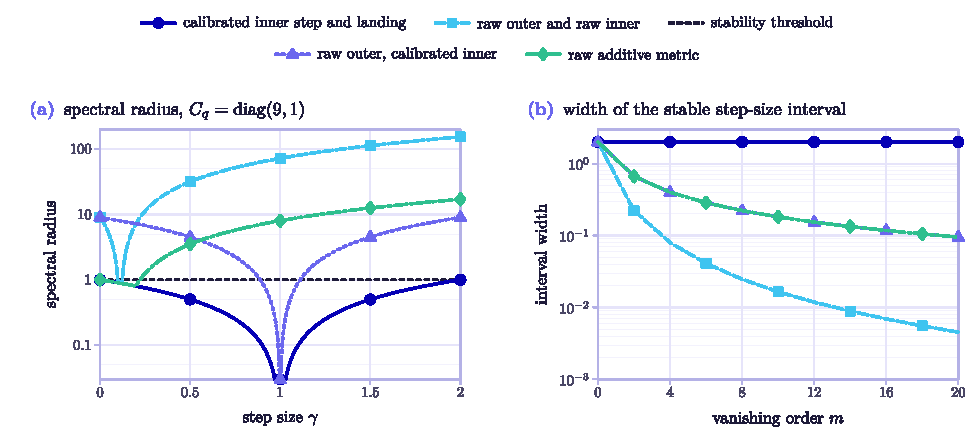
\includegraphics[width=\linewidth]{figures/conditioning.pdf}
  \caption{Exact local linear stability.  (a) Spectral radius versus method-specific step size for $C_q=\diag(9,1)$; values below $0.03$ are shown at the display floor, and the dashed horizontal line marks stability radius one.  (b) Width of the exact stable step-size interval as the vanishing order increases.  The inner-only and raw-additive widths coincide, although their intervals have different locations.  In (a) the horizontal axis is the step size and the vertical axis is the spectral radius on a logarithmic scale; in (b) the horizontal axis is the vanishing order and the vertical axis is the interval width, also logarithmic.}
  \label{fig:conditioning}
\end{figure}

\subsection{Learned circle geometry}

Quadrature leaves open whether a learned Jacobian preserves the same separation between spectral range and scale.  We train a two-hidden-layer noise-conditional residual MLP by denoising regression at three noise levels and compute $\widehat H_\theta=\operatorname{sym}(\nabla D_\theta)$ from its analytic input Jacobian.  Both the uniform circle and the quadratic-zero circle use $12$ independent seeds.  Figure~\ref{fig:learned-circle} shows biased eigenvalues, most visibly at the smallest noise where local coverage is hardest, alongside an accurate top eigenspace.  The contrast is quantitative at the quadratic zero with $\sigma=0.12$: replacing raw $\widehat H_\theta$ by its hard top-one projector improves the median operator error by $1.483$, with paired percentile-bootstrap interval $[1.443,1.528]$, and improves all $12$ seeds; a two-sided sign test over the seeds gives $p=2^{-11}\approx4.9\times10^{-4}$, which we regard as the primary evidence here, since a percentile bootstrap for a median with $12$ replications is coarse and its interval largely reflects seed spread.  On this benchmark, tangent-range recovery is more accurate than eigenvalue recovery.

\begin{figure}[!htbp]
  \centering
  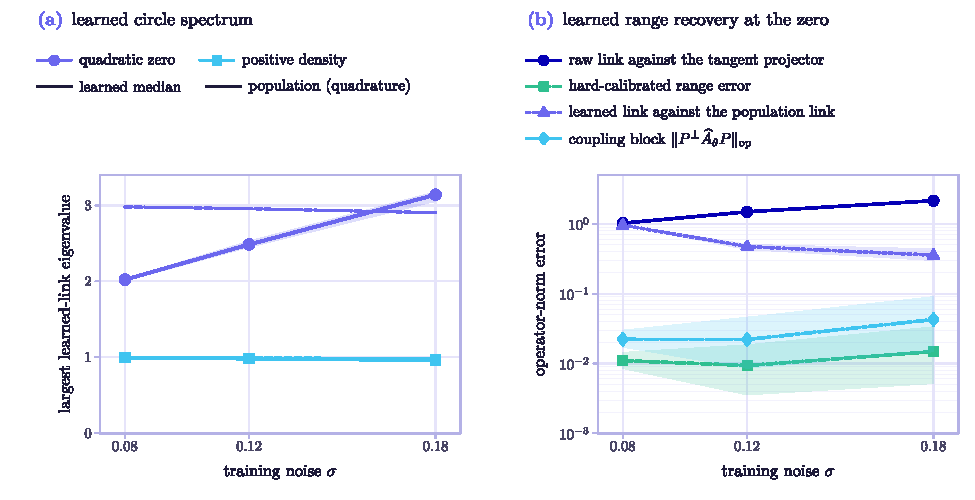
\includegraphics[width=\linewidth]{figures/learned-geometry.pdf}
  \caption{Twelve independently trained models per circle density ($24$ total); curves show medians and shaded bands show interquartile ranges.  (a) Largest learned-link eigenvalue for positive density and for a quadratic zero; solid curves are the learned medians and dashed curves the population values computed by deterministic quadrature.  (b) Four operator-norm errors at the zero: the raw link against the tangent projector, the hard-calibrated range error, the learned link against the finite-noise population link, and the tangent-normal coupling block $\|P^\perp\widehat A_\theta P\|_\op$ that replaces the full error in the residual bound~\eqref{eq:hard-residual}.  The learned spectrum is biased, while hard calibration gives substantially smaller operator error for the tangent range.  In both panels the horizontal axis is the training noise level; the vertical axis is the tangent eigenvalue in (a) and the operator-norm error on a logarithmic scale in (b).}
  \label{fig:learned-circle}
\end{figure}

\subsection{Rotated anisotropic finite-type plane}

The circle has $k=1,d=2$, so it cannot show whether calibration survives multiple tangent directions, anisotropy, and a larger ambient space.  We therefore use a fixed random orthonormal frame $U\in\R^{16\times2}$ and latent density
\begin{equation}
  \rho(z)\propto\bigl(z_1^4+0.1z_2^4\bigr)
  \exp\!\left(-\frac{\|z\|^2}{2(0.35)^2}\right),
  \qquad X=Uz.
  \label{eq:learned-plane-density}
\end{equation}
The resulting order-four zero has unequal population tangent eigenvalues and a nonzero tangent-normal eigengap.  Over the same $12$ seeds, Figure~\ref{fig:learned-plane} and Table~\ref{tab:learned-midscale} report both learned-link eigenvalues and projector error, keeping eigenvalue scale separate from tangent alignment.  At $\sigma=0.18$, hard top-two calibration lowers the median projector error from $1.314$ to $0.016$.  The paired median improvement is $1.301$, with bootstrap interval $[1.266,1.603]$, and every seed improves, again $p=2^{-11}$ by the sign test.  The fixed soft filter with $\tau=0.25$ reduces raw scaling error, but it is not an orthogonal projector.

Table~\ref{tab:calibration-regime} identifies which guarantee is actually in force.  At this noise level the learned link is $\eta=1.355$ from the population link in operator norm, against a threshold $c_q/2=0.539$, so the hypothesis of Proposition~\ref{prop:hard} fails by a factor of about $2.5$ and the bound \eqref{eq:hard-bound} is vacuous; the two circle settings satisfy it.  The accuracy observed on the plane is therefore not an instance of that bound.  It is explained by the residual form \eqref{eq:hard-residual}: the tangent-normal coupling block measures only $\|P^\perp\widehat A_\theta P\|_\op=0.0374$, a factor of $36$ below the full operator-norm error, and the computed separation $\delta(\widehat A_\theta)=0.840$ stays positive, so \eqref{eq:hard-residual} certifies $0.0422$ against an observed $0.0160$.  The learned error at a finite-type zero is thus concentrated in eigenvalue scale rather than in the eigenvectors, which is exactly the structure the operator-norm bound cannot exploit and the residual bound can.  On the two circles the residual bound is attained to three decimal places.

The population spectrum at these noise levels is itself pre-asymptotic, which bounds what this experiment can test.  Because the latent density in \eqref{eq:learned-plane-density} is a degree-four tilt of an isotropic Gaussian envelope of scale $s=0.35$, homogeneity of $q_4$ makes the tilt scale free and gives $H_\sigma(p)=\tfrac{s^2}{s^2+\sigma^2}\,UC_qU^\top$ exactly, with $C_q=\diag(4.636,1.364)$ and $\tr C_q=k+m=6$.  At $\sigma=0.12$, $0.18$, and $0.25$ the scalar factor is $0.895$, $0.791$, and $0.662$, so the population traces are $5.37$, $4.75$, and $3.97$ rather than $6$.  Rounding the trace statistic would return the correct order only for $\sigma<0.106$, below every noise level trained here.  Comparisons on this problem are therefore made against the exact finite-noise population operator rather than against its limit, and the experiment tests anisotropic range recovery and calibration rather than the asymptotic trace law; the circle experiments test the trace law directly.

\begin{figure}[!htbp]
  \centering
  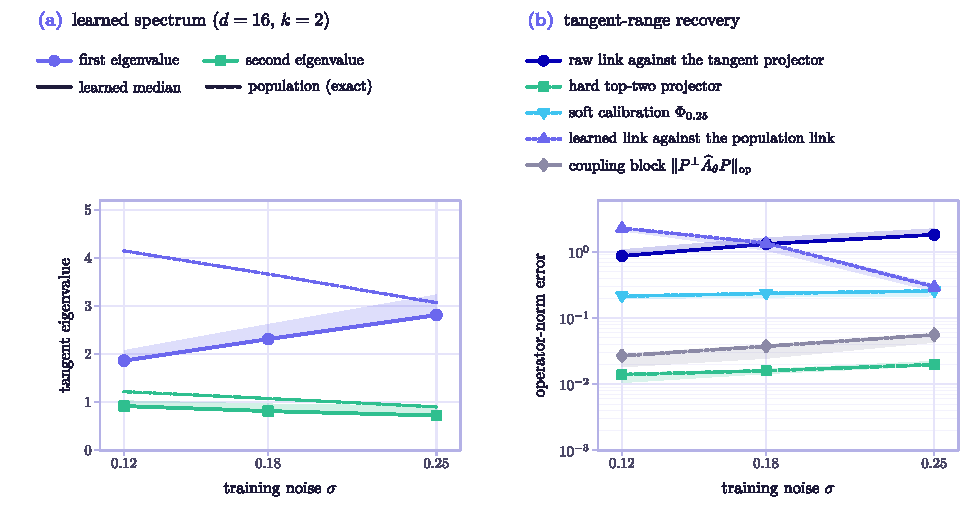
\includegraphics[width=\linewidth]{figures/learned-plane.pdf}
  \caption{Twelve independently trained denoisers for the rotated $d=16,k=2$ order-four model.  (a) The two largest learned-link eigenvalues, solid, against the exact finite-noise population tangent eigenvalues, dashed.  (b) Five operator-norm errors: the raw link, the hard top-two projector, the soft calibration $\Phi_{0.25}$, the learned link against the population link, and the tangent-normal coupling block $\|P^\perp\widehat A_\theta P\|_\op$ of the residual bound~\eqref{eq:hard-residual}.  Bands are interquartile ranges.  In both panels the horizontal axis is the training noise level; the vertical axis is the tangent eigenvalue in (a) and the operator-norm error on a logarithmic scale in (b).}
  \label{fig:learned-plane}
\end{figure}

\begin{table}[!htbp]
  \centering
  \caption{Learned geometry at the middle training noise.  Entries are medians with interquartile ranges over $12$ independent seeds.  Errors are operator norms relative to the true tangent projector.  The last column thresholds learned eigenvalues at $1/2$; it is a diagnostic, not an adaptive-rank guarantee.}
  \label{tab:learned-midscale}
  \small
  \setlength{\tabcolsep}{3.5pt}
  \begin{tabular}{@{}l r c c c c@{}}
    \toprule
    Setting & \shortstack[c]{Population\\spectrum}
      & \shortstack[c]{Largest learned-link\\spectrum [IQR]}
      & \shortstack[c]{Raw error\\\mbox{[IQR]}}
      & \shortstack[c]{Hard error\\\mbox{[IQR]}}
      & \shortstack[c]{Rank\\success} \\
    \midrule
    Positive circle, $0.12$
      & $0.993$ & $0.983\ [0.974,0.996]$ & $0.046\ [0.036,0.066]$ & $0.008\ [0.006,0.021]$ & $12/12$ \\
    \addlinespace[2pt]
    Zero circle, $0.12$
      & $2.957$ & $2.485\ [2.449,2.532]$ & $1.485\ [1.449,1.532]$ & $0.009\ [0.004,0.019]$ & $12/12$ \\
    \addlinespace[2pt]
    \multirow{2}{*}{Rotated plane, $0.18$}
      & $3.667$ & $2.314\ [2.282,2.619]$
      & \multirow{2}{*}{$1.314\ [1.282,1.619]$}
      & \multirow{2}{*}{$0.016\ [0.014,0.017]$}
      & \multirow{2}{*}{$12/12$} \\
      & $1.078$ & $0.816\ [0.808,0.965]$ & & & \\
    \bottomrule
  \end{tabular}
\end{table}

\begin{table}[!htbp]
  \centering
  \caption{Which calibration guarantee is in force at the middle training noise.  Medians over $12$ seeds.  Here $\eta=\|\widehat A_\theta-H_\sigma\|_\op$ is the quantity constrained by Proposition~\ref{prop:hard}, whose operator-norm bound \eqref{eq:hard-bound} requires $\eta<c_q/2$ and is reported as vacuous when it exceeds one.  The residual bound \eqref{eq:hard-residual} replaces $\eta$ by the tangent-normal coupling block $\|P^\perp\widehat A_\theta P\|_\op$ and divides by the computed separation $\delta(\widehat A_\theta)$ of \eqref{eq:computed-separation}.  The plane fails the operator-norm hypothesis while the residual bound remains informative there.}
  \label{tab:calibration-regime}
  \small
  \setlength{\tabcolsep}{4pt}
  \begin{tabular}{@{}lccccccc@{}}
    \toprule
    Setting & $\eta$ & $c_q/2$ & \shortstack{Bound\\\eqref{eq:hard-bound}}
      & $\|P^\perp\widehat A_\theta P\|_\op$ & $\delta(\widehat A_\theta)$
      & \shortstack{Bound\\\eqref{eq:hard-residual}}
      & \shortstack{Observed\\hard error} \\
    \midrule
    Positive circle, $0.12$
      & $0.042$ & $0.496$ & $0.084$
      & $0.0077$ & $0.948$ & $0.0081$ & $0.0081$ \\
    Zero circle, $0.12$
      & $0.471$ & $1.478$ & $0.319$
      & $0.0221$ & $2.461$ & $0.0094$ & $0.0094$ \\
    Rotated plane, $0.18$
      & $1.355$ & $0.539$ & vacuous
      & $0.0374$ & $0.840$ & $0.0422$ & $0.0160$ \\
    \bottomrule
  \end{tabular}
\end{table}

\subsection{End-to-end learned optimization ablation}

The final experiment places the learned geometric estimates inside SC-DRGD on the quadratic-zero circle and rotated plane.  We compare four variants: oracle Riemannian gradient descent, a raw link followed by the raw denoiser, hard calibration only in the inner step, and hard calibration in both the step and normal-only learned landing.  Figure~\ref{fig:learned-optimization} gives each method its own step-size sweep.  On the circle, the reported gap is the projected objective $F(x_t)-F(p)=f(\pi(x_t))-f(p)$ from Theorem~\ref{thm:optimization}, with feasibility reported separately.  Both objectives have ambient gradient zero at the target, as required by Corollary~\ref{cor:local-invariant}.

Using the descriptive criterion of median final gap below $10^{-3}$ and median feasibility error below $0.1$, SC-DRGD succeeds at $19/20$ tested circle step sizes and $23/24$ plane step sizes.  The corresponding counts are $0/20$ and $0/24$ for the raw method, and $7/20$ and $12/24$ for the inner-only ablation.  Two checks indicate that these counts are not artifacts of aggregating by the median or of the particular threshold.  Per-seed success rates, averaged over the tested step sizes, are $95.0\%$, $35.8\%$, and $12.1\%$ on the circle and $95.8\%$, $50.3\%$, and $3.8\%$ on the plane, in the same order.  Loosening the gap threshold to $10^{-2}$ gives circle counts $20/20$, $9/20$, and $7/20$, and tightening it to $10^{-4}$ gives $19/20$, $4/20$, and $0/20$; the ordering is unchanged throughout.

The counts track the exact linear stability intervals of Section~\ref{sec:stability} more closely than the criterion alone suggests.  At $\sigma=0.12$ the population tangent eigenvalue is $c=2.957$, so those intervals are $((c-1)/c^2,(c+1)/c^2)=(0.224,0.453)$ for the raw additive update, $(1-1/c,1+1/c)=(0.662,1.338)$ for inner-only calibration, and $(0,2)$ after full calibration.  The circle grid places $5$, $7$, and $20$ of its $20$ step sizes inside these intervals, against observed counts of $0$, $7$, and $19$.  Inner-only calibration therefore agrees with the linearization exactly, and full calibration agrees at every step size but one.

The residual disagreements have different causes, which the criterion does not separate.  The single calibrated failure is the smallest step size, $\gamma=0.05$, in both sweeps; there the median gap is still halving over the final fifth of the run, so the horizon of $35$ and $30$ steps is binding rather than stability.  The raw method instead remains stable inside its own interval while converging to a biased point: at its five in-interval step sizes the median final gap lies between $5.4\times10^{-2}$ and $8.2\times10^{-2}$, above the criterion at every threshold tested.  Its $0/20$ therefore records density-dependent bias rather than divergence, which is the effect calibration is intended to remove.  These grid counts describe this benchmark and are not universal stability guarantees.

Because each denoiser is noise conditional and trained at three levels, the same models can be run at every trained level without retraining, which tests the noise dependence that Corollary~\ref{cor:local-invariant} predicts.  Taking for each noise level the smallest median final value over the step-size grid, the feasibility floor of SC-DRGD is $6.7\times10^{-3}$, $1.7\times10^{-2}$, and $6.1\times10^{-2}$ at $\sigma=0.08,0.12,0.18$ on the circle, and $1.2\times10^{-3}$, $3.5\times10^{-3}$, and $1.2\times10^{-2}$ at $\sigma=0.12,0.18,0.25$ on the plane.  Fitting a power law over each range gives exponents $2.7$ and $3.2$.  The theory predicts an $O(\sigma^2)$ floor, which is an upper bound, so decay at least this fast is consistent with it; the ratios $\text{feasibility}/\sigma^2$ stay within a factor of two over the circle range and a factor of $2.4$ over the plane range.  The objective gap is not a useful floor diagnostic on these problems, since the calibrated iteration contracts it to $10^{-10}$ or below within the horizon and the residual is set by the number of iterations rather than by $\sigma$.

\begin{figure}[!htbp]
  \centering
  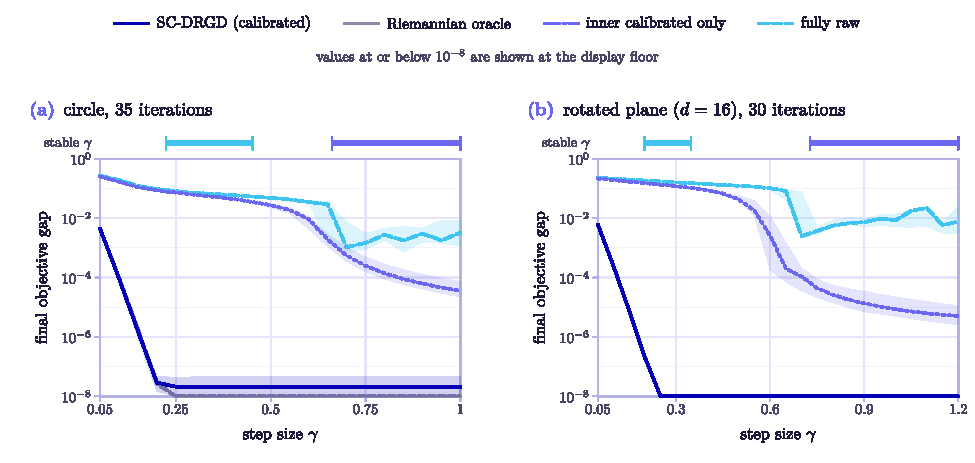
\includegraphics[width=\linewidth]{figures/learned-optimization.pdf}
  \caption{End-to-end learned optimization over method-specific step-size sweeps.  Curves are median final objective gaps and bands are interquartile ranges over $12$ independently trained models per problem; dashed gray is oracle Riemannian gradient descent.  Left: quadratic-zero circle after $35$ steps.  Right: rotated order-four plane after $30$ steps.  Values at or below $10^{-8}$ are shown at the display floor.  The horizontal axis is the step size and the vertical axis is the final objective gap on a logarithmic scale.  Shading inside each panel is the interquartile range and nothing else.  The two bars above each panel, marked \emph{stable} $\gamma$, are annotations rather than data: they give the exact linear stability intervals of Section~\ref{sec:stability} at the plotted noise level, cyan for the fully raw update and violet for inner-only calibration.  The fully calibrated interval is $(0,2)$ and covers each panel entirely, so it is not drawn.  The inner-only curve descends where its bar begins, whereas the raw update is stable throughout its own bar yet converges to a biased point there.  Stability and accuracy therefore separate for the raw update, which is what calibration removes.}
  \label{fig:learned-optimization}
\end{figure}

\FloatBarrier

\section{Limitations and scope}
\label{sec:roadmap}

\paragraph{Limits of the assumptions.}
The finite-type assumption is substantive.  For an infinitely flat one-dimensional density such as $\rho(u)\asymp e^{-1/u^2}$, Laplace's method gives typical $u^2\asymp\sigma$ and hence $\sigma^{-2}\Cov(X\mid Y=p)=\Theta(\sigma^{-1})$.  For this example, the tangent metric has no finite limit.  Definition~\ref{def:finite} is also narrower than the argument requires in a second way: it asks for a polynomial leading jet, so effective densities vanishing at a finite but non-even order, such as $\|z\|^{3}$ or $\|z\|^{1/2}$, are excluded even though the limit and the trace law hold for them.  Extending the uniform eigengap of Lemma~\ref{lem:universal-gap} beyond polynomial jets is open.  Boundaries and singular supports pose a different problem, since their local geometry is described by tangent cones rather than tangent spaces.  Appendix~\ref{app:flat} works that case out in full.

Theorem~\ref{thm:finite} is also local.  A full learning guarantee would need uniform control of the population biases $\beta_H,\beta_L$, the eigengap, and the optimizer's visited set.  It would further have to turn denoising training risk, typically an $L^2$ quantity, into the local score-Jacobian errors required by Corollary~\ref{cor:learned}.

\paragraph{Coverage of the experiments.}
The learned studies are controlled synthetic tests.  They provide no evidence yet for a large pretrained diffusion model or real data.  Every experiment has ambient dimension $d\le16$ and intrinsic dimension $k\le2$, and the population and finite-sample studies are $d=2$, $k=1$ throughout.  Two jet families are tested, the radial $\theta^{2r}$ on the circle and one anisotropic quartic on the plane, and that plane is affine, so every curvature-dependent term in Theorem~\ref{thm:normal-boundary} vanishes on it.  Appendix~\ref{app:spiral} partly closes this by placing a finite-type zero on a spiral whose curvature varies by a factor of five along the arc, where the limit is still $k+m$ and the $O(\sigma^2)$ remainder is found to scale as the square of the curvature $\kappa$; that check is nonetheless still $k=1$, so curvature combined with several tangent directions remains untested.  A single random frame $U$ was drawn; because the construction is equivariant under rotation this is not a loss of generality, but it does mean frame-to-frame variability is not sampled.  Hard calibration uses the known value of $k$, while the fixed threshold is reported only as a rank diagnostic.  Because the largest learned-link eigenvalues can remain materially biased even when the eigenspace is accurate, the trace law is not a reliable empirical estimator of vanishing order without further sample and Jacobian control.  Query-focused resampling depends only on the noisy input and therefore preserves the population conditional mean, but it remains part of the benchmark design.  Larger architectures, adaptive eigengap selection, and real-data validation are open empirical questions.

The population claims can be checked directly against the $q_m$-tilted Gaussian spectrum, trace law, and density-floor crossover.  For a learned Jacobian, Proposition~\ref{prop:hard} guarantees stable calibration when estimation error is sufficiently smaller than the tangent-normal eigengap.  It makes no converse claim once the error becomes comparable to the gap.  The per-seed tables include failures as well as successes, allowing the empirical behavior to be inspected without relying on plotted medians.

\paragraph{Practical scope.}
Low-probability regions can change the scale of score-derived geometry, including when an optimizer leaves high-density modes.  Calibration addresses that geometric effect.  It does not certify that a learned manifold represents valid or safe designs; domain constraints and downstream validation remain necessary.

\section{Conclusion}

At a regular positive-density point, the denoiser-Jacobian limit is the tangent projector.  At a finite-type zero, its range and nonzero eigenvalue scale have different interpretations.  The limit is $UC_{q_m}U^\top$: its range is the tangent space, while its positive eigenvalues depend on the leading density jet and sum to $k+m$.  The density-floor calculation and the $O(\sigma)$ moving-query analysis give explicit transition laws and identify where this distinction persists.

When population bias and learned-Jacobian error are below the tangent-normal eigengap, spectral projection estimates the tangent projector with controlled error.  The optimization analysis treats calibration in both the tangent update and the landing map, and the experiments compare this choice with partially calibrated and raw variants.  Population quadrature, finite-sample posterior estimation, and learned-denoiser experiments exhibit the predicted separation between tangent range and eigenvalue scale.  In the finite-type small-noise limit, the nonzero eigenspace retains tangent geometry, whereas the raw eigenvalue scale remains density dependent.

\bibliographystyle{plainnat}
\bibliography{references}

\appendix
\section{Notation}
\label{app:notation}

Recurring symbols are collected here in order of first appearance.  Each is also
defined at its first use in the text.  Throughout, $\|\cdot\|$ is the Euclidean
norm on vectors and $\|\cdot\|_\op$ the operator norm on matrices.

\begin{longtable}{@{}p{0.20\linewidth}p{0.76\linewidth}@{}}
\toprule
\endfirsthead
\toprule
\endhead
\multicolumn{2}{@{}l}{\emph{Manifold and ambient geometry}}\\
\midrule
$\M$, $k$, $d$ & Embedded $C^3$ manifold without boundary, its dimension, and the ambient dimension, with $1\le k<d$.\\\addlinespace[3pt]
$\T_p\M$, $\N_p\M$ & Tangent and normal spaces at $p\in\M$.\\\addlinespace[3pt]
$U_p$, $U_\perp$ & Matrices with orthonormal columns spanning $\T_p\M$ and $\N_p\M$; $P=U_pU_p^\top$ and $P^\perp=I_d-P$.\\\addlinespace[3pt]
$F_p$, $g_p$, $J_p$ & Normal graph chart at $p$, its normal component, and the area Jacobian $\sqrt{\det(DF_p^\top DF_p)}$.\\\addlinespace[3pt]
$\mathrm{II}_p$, $S_b$, $\mathcal B_a$ & Second fundamental form; shape operator in the normal direction $b$; the map $v\mapsto\mathrm{II}_p[a,v]$.\\\addlinespace[3pt]
$\kappa$ & Curvature of a one-dimensional manifold, used only in Appendix~\ref{app:spiral}.\\\addlinespace[3pt]
$\mathcal T_r$, $\pi$ & Reach tube $\{x:\dist(x,\M)<r\}$ and nearest-point projection onto $\M$.\\\addlinespace[3pt]
\addlinespace
\multicolumn{2}{@{}l}{\emph{Density and its leading jet}}\\
\midrule
$\mu$, $\rho$ & Law of the clean variable $X$ and its density with respect to Riemannian volume.\\\addlinespace[3pt]
$a_p$ & Effective chart density $\rho(F_p(z))J_p(z)$, whose jets drive every limit.\\\addlinespace[3pt]
$q_m$, $m$ & First nonzero homogeneous jet of $a_p$ and its degree, the vanishing order.\\\addlinespace[3pt]
$\mathcal Z_q$, $C_{q_m}$ & Normalizer $\int q_me^{-\|u\|^2/2}du$ and the covariance \eqref{eq:Cq} of the $q_m$-tilted Gaussian.\\\addlinespace[3pt]
\addlinespace
\multicolumn{2}{@{}l}{\emph{Noise, score and denoiser}}\\
\midrule
$\sigma$, $Y_\sigma$, $p_\sigma$ & Noise scale, the observation $X+\sigma G$, and its density.\\\addlinespace[3pt]
$s_\sigma$, $D_\sigma$, $H_\sigma$ & Score $\nabla\log p_\sigma$, denoiser $y+\sigma^2s_\sigma$, and link Hessian $\nabla D_\sigma=\sigma^{-2}\Cov(X\mid Y_\sigma=y)$.\\\addlinespace[3pt]
$s_\theta$, $\widehat A_\theta$ & Learned score and its symmetrized link Jacobian.\\\addlinespace[3pt]
\addlinespace
\multicolumn{2}{@{}l}{\emph{Spectral calibration}}\\
\midrule
$A_0$, $c_q$ & Limiting operator $U_pC_{q_m}U_p^\top$ and its smallest nonzero eigenvalue $\lambda_{\min}(C_{q_m})$.\\\addlinespace[3pt]
$\mathcal P_k$, $Q_\sigma$ & Orthogonal projector onto a top-$k$ eigenspace, and $\mathcal P_k(H_\sigma)$.\\\addlinespace[3pt]
$\eta$, $\delta(\widehat A)$ & Operator-norm estimation error $\|\widehat A-A_0\|_\op$ and the computed separation \eqref{eq:computed-separation}.\\\addlinespace[3pt]
$\vartheta_{\mathrm{sp}}$, $\tau$, $\Phi_\tau$ & Hard spectral cutoff, soft filter strength, and the filter $\widehat A(\widehat A+\tau I)^{-1}$.\\\addlinespace[3pt]
\addlinespace
\multicolumn{2}{@{}l}{\emph{Boundary layer at a finite-type point}}\\
\midrule
$a$, $b$ & Rescaled tangential and normal coordinates of a query, so the query is $F_p(\sigma a)+\sigma b$.\\\addlinespace[3pt]
$\nu_{q,a}$, $C_a$, $\mu_a$ & Shifted tilted law with density $\propto q_m(a+u)e^{-\|u\|^2/2}$, its covariance and its mean.\\\addlinespace[3pt]
$\Gamma_a$, $\Lambda_a$ & Normal-valued covariance \eqref{eq:normal-boundary-objects} and its calibrated version $\Gamma_aC_a^{-1}$.\\\addlinespace[3pt]
$K_T$, $K_N$, $c_0$ & Compact sets of admissible $a$ and $b$, and $\inf_{a\in K_T}\lambda_{\min}(C_a)$.\\\addlinespace[3pt]
\addlinespace
\multicolumn{2}{@{}l}{\emph{Optimization}}\\
\midrule
$f$, $F$, $\gamma$ & Ambient objective, its pullback $f\circ\pi$, and the step size.\\\addlinespace[3pt]
$L$, $Q$, $\overline D_Q$ & Landing map, tangent projector oracle, and the normal-only landing \eqref{eq:normal-landing}.\\\addlinespace[3pt]
$\eps_P$, $\eps_L$ & Oracle errors of Assumption~\ref{ass:oracles}, for the projector and the landing map.\\\addlinespace[3pt]
$\beta_H$, $\beta_L$, $g_\sigma$ & Population Jacobian bias, population landing bias, and tangent-normal eigengap, all defined in Corollary~\ref{cor:learned}.\\\addlinespace[3pt]
$\eps_s$, $\eps_J$, $R_D$ & Uniform score error, score-Jacobian error, and a bound on $\|D_\sigma(y)-y\|$.\\\addlinespace[3pt]
$\mathcal V$ & Query set containing every iterate $x_t$ and intermediate point $z_t$.\\\addlinespace[3pt]
$B$, $L_f$, $L_F$, $L_\pi$, $K_\pi$ & Gradient bound and Lipschitz constants of $\nabla f$, $\nabla F$, $\pi$ and $\mathrm d\pi$.\\\addlinespace[3pt]
$G_f$ & Tangent block $U_p^\top\nabla^2f(p)U_p$ of the ambient Hessian.\\\addlinespace[3pt]
\bottomrule
\end{longtable}

\section{Exact posterior identities}
\label{app:tweedie}

For Proposition~\ref{prop:tweedie}, let
\[
  \varphi_\sigma(y-x)
  =(2\pi\sigma^2)^{-d/2}
  \exp\!\left(-\frac{\|y-x\|^2}{2\sigma^2}\right).
\]
The Gaussian factor and all of its derivatives are bounded as functions of $x$ for fixed $\sigma>0$.  Since $\mu$ is finite, differentiation under the integral is justified by dominated convergence.  We obtain
\begin{align}
  \nabla p_\sigma(y)
  &=\int \frac{x-y}{\sigma^2}\varphi_\sigma(y-x)\,\mu(dx),\\
  \nabla\log p_\sigma(y)
  &=\frac{\E[X\mid Y_\sigma=y]-y}{\sigma^2}.
\end{align}
This is the posterior-mean identity.

To differentiate the conditional mean, write $m(y)=\E[X\mid Y_\sigma=y]$.  In coordinates,
\begin{align}
  \partial_{y_j}m_i(y)
  &=
  \frac{1}{\sigma^2}
  \left(
  \E[X_iX_j\mid Y_\sigma=y]
  -\E[X_i\mid Y_\sigma=y]\E[X_j\mid Y_\sigma=y]
  \right).
\end{align}
Therefore $\nabla m(y)=\sigma^{-2}\Cov(X\mid Y_\sigma=y)$.  Since $m=D_\sigma$, differentiating \eqref{eq:link} proves the second identity and symmetry of $H_\sigma$.

\section{A localized Laplace expansion}
\label{app:laplace}

In the normal graph \eqref{eq:chart}, assume
\begin{align}
  g_p(z)&=\tfrac12\mathrm{II}_p[z,z]+R_g(z),
  &\|R_g(z)\|&\le C\|z\|^3,\label{eq:normal-exp}\\
  a_p(z)&=q_m(z)+q_{m+1}(z)+R_a(z),
  &|R_a(z)|&\le C\|z\|^{m+2}.\label{eq:density-exp-app}
\end{align}
Here $\mathrm{II}_p:\R^k\times\R^k\to\N_p\M$ is the second fundamental form in the chosen frame.  The normal graph is orthogonal to $U_pz$, so
\begin{equation}
  \|F_p(z)-p\|^2=\|z\|^2+\|g_p(z)\|^2
  =\|z\|^2+O(\|z\|^4).
  \label{eq:distance-exp}
\end{equation}

Choose the chart so that $\M\cap B(p,\eta)$ is contained in its image.  The contribution from $\M\setminus B(p,\eta)$ to a posterior moment of order $s\in\{0,1,2\}$ is at most
\begin{equation}
  O\!\left(e^{-\eta^2/(4\sigma^2)}\right),
  \label{eq:tail-localization}
\end{equation}
after absorbing a bounded polynomial factor into the exponential.  This term is smaller than every power of $\sigma$.

Inside the chart set $z=\sigma u$.  For $\|u\|<\eta/\sigma$,
\begin{align}
  \sigma^{-m}a_p(\sigma u)
  &=q_m(u)+\sigma q_{m+1}(u)
    +O(\sigma^2\|u\|^{m+2}),\label{eq:density-scale}\\
  \exp\!\left(-\frac{\|g_p(\sigma u)\|^2}{2\sigma^2}\right)
  &=1+O(\sigma^2\|u\|^4).\label{eq:kernel-scale}
\end{align}
The expansion \eqref{eq:kernel-scale} is to be read on bounded sets of $u$; on the whole chart, where $\|u\|$ may reach $\eta/\sigma$, the elementary bound $|e^{-t}-1|\le t$ for $t\ge0$ gives instead $0\le1-\exp(-\|g_p(\sigma u)\|^2/2\sigma^2)\le C\sigma^2\|u\|^4$ with the same constant, and $\|g_p(\sigma u)\|\le C\sigma^2\|u\|^2$ makes the exponent nonnegative, so the factor never exceeds one.  On a smaller fixed chart, these remainders are dominated by a polynomial in $\|u\|$ times $e^{-c\|u\|^2}$.  The annulus between that smaller chart and the original one is exponentially negligible.  Dominated convergence therefore permits termwise integration over $\R^k$.

Let
\[
  \mathcal Z_q=\int_{\R^k}q_m(u)e^{-\|u\|^2/2}\,du
  =(2\pi)^{k/2}\,\E[q_m(Z)],\qquad Z\sim\cN(0,I_k).
\]
The unnormalized $\mathcal Z_q$ and the expectation $\E[q_m(Z)]$ used in
\eqref{eq:Cq} therefore differ by the Gaussian normalizing constant, which
cancels in every ratio below.  Because $q_m$ is even and $q_{m+1}$ is odd,
\begin{equation}
  \int_\M e^{-\|x-p\|^2/(2\sigma^2)}\,\mu(dx)
  =\sigma^{k+m}\bigl(\mathcal Z_q+O(\sigma^2)\bigr).
  \label{eq:normalizer-exp}
\end{equation}
The order-$\sigma$ term vanishes by parity.  Multiplication by the ambient Gaussian normalization gives
\begin{equation}
  p_\sigma(p)
  =(2\pi)^{-d/2}\mathcal Z_q\,
  \sigma^{k+m-d}\bigl(1+O(\sigma^2)\bigr).
  \label{eq:noisy-density-scaling}
\end{equation}
The smoothed-density power law therefore contains the vanishing order.

\section{Proof of the finite-type theorem}
\label{app:finite-proof}

\subsection{Parity and positivity}

For every fixed $u$,
\[
  q_m(u)=\lim_{t\downarrow0}\frac{a_p(tu)}{t^m}\ge0.
\]
If $m$ were odd, homogeneity would give $q_m(-u)=-q_m(u)$.  Nonnegativity in both directions would imply $q_m\equiv0$, a contradiction.  Hence $m$ is even, $q_m$ is even, and it is positive on some nonempty open set.  In particular $\mathcal Z_q>0$.

\subsection{Posterior mean}

Let $N_1$ denote the unnormalized first centered moment about $p$.  Its tangent component is
\begin{align}
  P_{\T_p\M}N_1
  &=
  U_p\sigma^{k+m+1}
  \int_{\R^k}u
  \bigl(q_m(u)+\sigma q_{m+1}(u)+O(\sigma^2\operatorname{poly}(u))\bigr)
  e^{-\|u\|^2/2}\,du\nonumber\\
  &=
  U_p\sigma^{k+m+2}
  \int_{\R^k}u q_{m+1}(u)e^{-\|u\|^2/2}\,du
  +O(\sigma^{k+m+3}).
  \label{eq:tangent-first}
\end{align}
The leading integral vanishes because $u q_m(u)$ is odd.  From \eqref{eq:normal-exp}, the normal component is
\begin{equation}
  P_{\N_p\M}N_1
  =
  \frac{\sigma^{k+m+2}}{2}
  \int_{\R^k}\mathrm{II}_p[u,u]q_m(u)e^{-\|u\|^2/2}\,du
  +O(\sigma^{k+m+3}).
  \label{eq:normal-first}
\end{equation}
Dividing \eqref{eq:tangent-first} and \eqref{eq:normal-first} by \eqref{eq:normalizer-exp} yields \eqref{eq:meanlimit}, with
\begin{equation}
  b_{p,q}
  =
  U_p\frac{\int u q_{m+1}(u)e^{-\|u\|^2/2}\,du}{\mathcal Z_q}
  +\frac12
  \frac{\int \mathrm{II}_p[u,u]q_m(u)e^{-\|u\|^2/2}\,du}{\mathcal Z_q}.
  \label{eq:b-explicit}
\end{equation}

\subsection{Posterior covariance}

Write $N_0$ for the normalizer \eqref{eq:normalizer-exp} and $N_2$ for the
unnormalized second moment about $p$,
\begin{equation}
  N_0=\int_\M e^{-\|x-p\|^2/(2\sigma^2)}\mu(dx),
  \qquad
  N_2=\int_\M(x-p)(x-p)^\top e^{-\|x-p\|^2/(2\sigma^2)}\mu(dx),
  \label{eq:n0-n2}
\end{equation}
so that $\E[(X-p)(X-p)^\top\mid Y_\sigma=p]=N_2/N_0$.  We compute the three
blocks of $N_2$ and then divide.

In the chart, $\mu(dx)=a_p(z)\,dz$ and $z=\sigma u$ gives $dz=\sigma^k du$, while
\eqref{eq:distance-exp} splits the kernel as
\begin{equation}
  e^{-\|F_p(\sigma u)-p\|^2/(2\sigma^2)}
  =e^{-\|u\|^2/2}\,
   \exp\!\left(-\frac{\|g_p(\sigma u)\|^2}{2\sigma^2}\right)
  =e^{-\|u\|^2/2}\bigl(1+O(\sigma^2\|u\|^4)\bigr),
  \label{eq:kernel-split}
\end{equation}
by \eqref{eq:kernel-scale}.  Combining this with \eqref{eq:density-scale}, the
unnormalized measure element is
\begin{equation}
  a_p(\sigma u)\,\sigma^k\,e^{-\|F_p(\sigma u)-p\|^2/(2\sigma^2)}\,du
  =\sigma^{k+m}
   \Bigl(q_m(u)+\sigma q_{m+1}(u)+O\bigl(\sigma^2\operatorname{poly}(u)\bigr)\Bigr)
   e^{-\|u\|^2/2}\,du,
  \label{eq:measure-element}
\end{equation}
the kernel remainder of \eqref{eq:kernel-split} having been absorbed into the
$O(\sigma^2\operatorname{poly}(u))$ term.  The displacement itself splits as
\begin{equation}
  x-p=U_p(\sigma u)+g_p(\sigma u),
  \qquad
  g_p(\sigma u)=\frac{\sigma^2}{2}\mathrm{II}_p[u,u]+O(\sigma^3\|u\|^3),
  \label{eq:displacement-split}
\end{equation}
using \eqref{eq:normal-exp}.

\emph{Tangent-tangent block.}  The tangent part of \eqref{eq:displacement-split}
contributes $\sigma^2U_puu^\top U_p^\top$, so by \eqref{eq:measure-element}
\begin{align}
  P_{\T_p\M}N_2P_{\T_p\M}
  &=\sigma^{k+m+2}U_p
    \int_{\R^k}uu^\top
    \Bigl(q_m(u)+\sigma q_{m+1}(u)+O\bigl(\sigma^2\operatorname{poly}(u)\bigr)\Bigr)
    e^{-\|u\|^2/2}\,du\;U_p^\top\nonumber\\
  &=\sigma^{k+m+2}U_p
    \left(\int_{\R^k}uu^\top q_m(u)e^{-\|u\|^2/2}\,du
    +O(\sigma^2)\right)U_p^\top.
  \label{eq:tt-second}
\end{align}
The order-$\sigma$ term drops because $uu^\top q_{m+1}(u)$ is odd, $uu^\top$
being even and $q_{m+1}$ odd.  The surviving integral is exactly
$\mathcal Z_qC_{q_m}$: writing $Z\sim\cN(0,I_k)$,
\begin{equation}
  \int_{\R^k}uu^\top q_m(u)e^{-\|u\|^2/2}\,du
  =(2\pi)^{k/2}\,\E\bigl[ZZ^\top q_m(Z)\bigr]
  =(2\pi)^{k/2}\,\E[q_m(Z)]\,C_{q_m}
  =\mathcal Z_qC_{q_m},
  \label{eq:tt-integral}
\end{equation}
where the middle step is the definition \eqref{eq:Cq} of $C_{q_m}$ and the last
is the definition of $\mathcal Z_q$.  Hence
\begin{equation}
  P_{\T_p\M}N_2P_{\T_p\M}
  =\sigma^{k+m+2}\mathcal Z_q
   \bigl(U_pC_{q_m}U_p^\top+O(\sigma^2)\bigr).
  \label{eq:tt-final}
\end{equation}

\emph{Tangent-normal block.}  Pairing the tangent part of
\eqref{eq:displacement-split} with the normal part gives a prefactor
$\sigma\cdot\sigma^2/2$, so
\begin{align}
  P_{\T_p\M}N_2P_{\N_p\M}
  &=\frac{\sigma^{k+m+3}}{2}U_p
    \int_{\R^k}u\,\mathrm{II}_p[u,u]^\top q_m(u)e^{-\|u\|^2/2}\,du
    +O(\sigma^{k+m+4})\nonumber\\
  &=O(\sigma^{k+m+4}).
  \label{eq:tn-second}
\end{align}
The displayed integral vanishes by parity: $u$ is odd while
$\mathrm{II}_p[u,u]$ and $q_m(u)$ are both even, so the integrand is odd.  The
nominal order-$\sigma^{k+m+3}$ term is therefore absent, and what remains comes
from the $O(\sigma^3\|u\|^3)$ remainder in \eqref{eq:displacement-split} and from
the $\sigma q_{m+1}$ term in \eqref{eq:measure-element}.

\emph{Normal-normal block.}  Both factors are normal, so by
\eqref{eq:displacement-split} the integrand carries $\|g_p(\sigma u)\|^2
=O(\sigma^4\|u\|^4)$ and
\begin{equation}
  P_{\N_p\M}N_2P_{\N_p\M}=O(\sigma^{k+m+4}).
  \label{eq:nn-second}
\end{equation}

\emph{Division and centering.}  Assembling \eqref{eq:tt-final},
\eqref{eq:tn-second} and \eqref{eq:nn-second}, and dividing by
$N_0=\sigma^{k+m}(\mathcal Z_q+O(\sigma^2))$ from \eqref{eq:normalizer-exp},
\begin{equation}
  \E\bigl[(X-p)(X-p)^\top\mid Y_\sigma=p\bigr]
  =\frac{N_2}{N_0}
  =\frac{\sigma^{k+m+2}\mathcal Z_q\bigl(U_pC_{q_m}U_p^\top+O(\sigma^2)\bigr)}
        {\sigma^{k+m}\bigl(\mathcal Z_q+O(\sigma^2)\bigr)}
  =\sigma^2U_pC_{q_m}U_p^\top+O(\sigma^4),
  \label{eq:second-moment-final}
\end{equation}
where the last step uses $\mathcal Z_q>0$ from Appendix~\ref{app:finite-proof}
and expands $(\mathcal Z_q+O(\sigma^2))^{-1}=\mathcal Z_q^{-1}(1+O(\sigma^2))$.
Finally $\eqref{eq:meanlimit}$ gives
$\E[X\mid Y_\sigma=p]-p=\sigma^2b_{p,q}+O(\sigma^3)$, so subtracting the outer
product of the mean removes only an $O(\sigma^4)$ matrix:
\begin{equation}
  \Cov(X\mid Y_\sigma=p)
  =\sigma^2U_pC_{q_m}U_p^\top+O(\sigma^4).
  \label{eq:cov-final}
\end{equation}
Dividing by $\sigma^2$ and applying Proposition~\ref{prop:tweedie} proves
\eqref{eq:hlimit}.

\subsection{Rank and trace}

For $v\ne0$,
\begin{equation}
  v^\top C_{q_m}v
  =
  \frac{\int(v^\top u)^2q_m(u)e^{-\|u\|^2/2}\,du}
  {\mathcal Z_q}>0.
\end{equation}
The strict inequality holds because $q_m$ is positive on an open set, which cannot be contained in the hyperplane $v^\top u=0$.  Hence $C_{q_m}\succ0$, and the ambient limit has rank $k$ and range $\T_p\M$.

Euler's identity gives $u^\top\nabla q_m(u)=m q_m(u)$.  Integrating the divergence of $u q_m(u)e^{-\|u\|^2/2}$ gives
\begin{align}
  0
  &=
  \int_{\R^k}
  \bigl(kq_m(u)+u^\top\nabla q_m(u)-\|u\|^2q_m(u)\bigr)
  e^{-\|u\|^2/2}\,du\\
  &=
  \int_{\R^k}
  \bigl(k+m-\|u\|^2\bigr)q_m(u)e^{-\|u\|^2/2}\,du.
\end{align}
Dividing by $\mathcal Z_q$ proves $\tr C_{q_m}=k+m$.

\subsection{Positive density and change of tangent frame}

If $\rho(p)>0$, then the first jet is the positive constant
$q_0=\rho(p)$ (the chart volume factor equals one at the origin).  Its
Gaussian tilt is unchanged, so $C_{q_0}=\E[ZZ^\top]=I_k$ and
$U_pC_{q_0}U_p^\top=P_{\T_p\M}$.

For coordinate invariance, let $\widetilde U_p=U_pO$ for $O\in O(k)$.
The same density jet in the new coordinates is
$\widetilde q_m(\widetilde z)=q_m(O\widetilde z)$.  Rotational invariance of
the standard Gaussian gives
\[
  C_{\widetilde q_m}=O^\top C_{q_m}O.
\]
It follows that
$\widetilde U_pC_{\widetilde q_m}\widetilde U_p^\top
=U_pC_{q_m}U_p^\top$, proving Corollary~\ref{cor:regular}.

\subsection{Minimal assumptions and rate assumptions}

The operator limit requires less regularity than the stated rate.  If
$g_p(z)=o(\|z\|)$ and $a_p(z)=q_m(z)+o(\|z\|^m)$, dominated convergence in the rescaled posterior gives
\[
  \sigma^{-2}\Cov(X\mid Y_\sigma=p)\to U_pC_{q_m}U_p^\top.
\]
For $D_\sigma(p)-p=O(\sigma^2)$ it suffices that $g_p(z)=O(\|z\|^2)$ and
$a_p(z)=q_m(z)+O(\|z\|^{m+1})$.  The sharper normalized-covariance error
$O(\sigma^2)$ requires the two-order expansion \eqref{eq:density-exp-app}, or a comparable assumption such as $a_p\in C^{m+1,1}$.

The additional rate assumptions are necessary.  For even $m$ and $0<\alpha<1$, the local one-dimensional density
\[
  a(z)=z^m\bigl(1+\operatorname{sgn}(z)|z|^\alpha\bigr)
\]
has posterior mean $\Theta(\sigma^{1+\alpha})$, rather than $O(\sigma^2)$.  Likewise
$a(z)=z^m(1+|z|^{1+\alpha})$ creates a
$\Theta(\sigma^{1+\alpha})$ correction to the normalized covariance.  Finite order alone gives convergence, not a universal polynomial remainder.

\subsection{A uniform finite-degree eigengap}

\begin{lemma}
\label{lem:universal-gap}
For fixed $k$ and even $m$, there is a constant $c_{k,m}>0$ such that
\[
  \lambda_{\min}(C_q)\ge c_{k,m}
\]
for every nonzero nonnegative homogeneous polynomial $q$ of degree $m$.
\end{lemma}

\begin{proof}
Normalize by $\E q(Z)=1$.  Homogeneous degree-$m$ polynomials form a finite-dimensional vector space, and the Gaussian $L^1$ norm is equivalent to any coefficient norm.  The normalized nonnegative polynomials therefore form a compact set.  The map
$q\mapsto\lambda_{\min}(\E[ZZ^\top q(Z)])$ is continuous and, by the positivity argument above, strictly positive at every point of that compact set.  It therefore has a positive minimum.
\end{proof}

The constant may deteriorate with $m$.  For a bounded collection
$m\le m_{\max}$, taking the minimum over the finitely many even degrees yields a uniform gap.  This gap applies on a controlled finite-type stratum; uniform spectral recovery also requires bounds on the Taylor remainders.

\section{Explicit examples and the full-support gap}
\label{app:examples}

\subsection{Radial and quadratic jets}

If $q_m(u)=\|u\|^m$, rotational invariance makes $C_q=cI_k$.  The trace identity gives $c=1+m/k$.  If
$q_2(u)=u^\top Au$ with $A\succeq0$ and $\tr A>0$, Isserlis' formula gives
\[
  \E[ZZ^\top(Z^\top AZ)]=(\tr A)I_k+2A,
  \qquad
  C_{q_2}=I_k+\frac{2A}{\tr A}.
\]

\subsection{Circle family}

For $x(\theta)=(\cos\theta,\sin\theta)$ and
$\rho_r(\theta)\propto(1-\cos\theta)^r$, the zero at $\theta=0$ has
$m=2r$ and $q_m(u)\propto u^{2r}$.  Hence
\[
  C_q
  =\frac{\E Z^{2r+2}}{\E Z^{2r}}
  =2r+1.
\]
For $r=1$, the posterior density in $\theta$ at $p=(1,0)$ is proportional to
\[
  (1-\cos\theta)
  \exp\!\left(-\frac{1-\cos\theta}{\sigma^2}\right).
\]
The rescaling $\theta=\sigma u$ gives
\begin{align}
  \E[X\mid Y_\sigma=p]
  &=p-\frac32\sigma^2(1,0)+O(\sigma^4),\\
  \Cov(X\mid Y_\sigma=p)
  &=3\sigma^2(0,1)(0,1)^\top+O(\sigma^4).
\end{align}
The density is smooth, nonnegative, and positive except at one point, so every open arc has positive mass and $\operatorname{supp}\mu=S^1$.  Equation \eqref{eq:circle-counter} follows, and the example shows that full support is weaker than a positive density lower bound.

\section{Two low-density crossover laws}
\label{app:crossovers}

\subsection{Changing the density floor}

The stated bound on mass outside the fixed neighborhood $U$ makes that contribution exponentially negligible after multiplication by the Gaussian kernel: an $\exp(o(\sigma^{-2}))$ mass factor is dominated by the fixed separation penalty $\exp(-c/\sigma^2)$.  Inside $U$, the uniform envelope on $r_\delta$ provides a Gaussian-integrable dominator after rescaling.  The local rescaling therefore determines the posterior.

In the setting of Theorem~\ref{thm:crossover}, substitute $z=\sigma u$ and divide the effective density by $\sigma^m$:
\[
  \sigma^{-m}a_{\delta_\sigma}(\sigma u)
  \longrightarrow q_m(u)+a_0\lambda.
\]
The rescaled tangent posterior therefore has density proportional to
$(q_m(u)+a_0\lambda)e^{-\|u\|^2/2}$.  Its mean is zero by parity, and its covariance is
\[
  \frac{a_0\lambda\E[ZZ^\top]+\E[ZZ^\top q_m(Z)]}
  {a_0\lambda+\E[q_m(Z)]},
\]
which is \eqref{eq:crossover}.  Taking the trace and using
$\tr C_q=k+m$ proves the second formula.  If
$\delta_\sigma/\sigma^m\to\infty$, dividing instead by $\delta_\sigma$ leaves the standard Gaussian law and covariance $I_k$.

For $a_\delta(\theta)=\delta+1-\cos\theta$, the local jet is
$q_2(u)=u^2/2$.  Here $\E q_2(Z)=1/2$ and
$\E[Z^2q_2(Z)]=3/2$, giving
\[
  C_{q,\lambda}=\frac{\lambda+3/2}{\lambda+1/2}.
\]

\subsection{Moving through a fixed distribution}

Let the query be $y_\sigma=F_p(\sigma a)$.  With the clean coordinate
$z=\sigma u$, the leading kernel becomes
\[
  \exp\!\left(-\frac12\|u-a\|^2\right),
\]
while the density contributes $\sigma^m q_m(u)$.  Dominated convergence shows that the rescaled tangent posterior converges to $\nu_{q,a}$, proving \eqref{eq:spatial}.

The rates used in Section~\ref{sec:optimization} follow under the stronger assumptions of Theorem~\ref{thm:finite}, uniformly for $a$ in a fixed compact set:
\begin{align}
  \sigma^{-m}a_p(\sigma u)
  &=q_m(u)+\sigma q_{m+1}(u)
    +O(\sigma^2\operatorname{poly}(u)),\\
  g_p(\sigma u)-g_p(\sigma a)
  &=\frac{\sigma^2}{2}
    \bigl(\mathrm{II}_p[u,u]-\mathrm{II}_p[a,a]\bigr)
    +O(\sigma^3\operatorname{poly}(u,a)).
\end{align}
The tangent and normal graph components are orthogonal, so
\begin{equation}
  \frac{\|F_p(\sigma u)-F_p(\sigma a)\|^2}{2\sigma^2}
  =\frac12\|u-a\|^2+O(\sigma^2\operatorname{poly}(u,a)).
\end{equation}
The same Gaussian domination as in Appendix~\ref{app:laplace} therefore shows that posterior tangent moments of order at most two differ from their $\nu_{q,a}$ limits by $O(\sigma)$.  Unlike at the centered query, the order-$\sigma$ term need not vanish because the shifted Gaussian breaks parity.  It follows that
\begin{equation}
  D_\sigma(F_p(\sigma a))-F_p(\sigma a)
  =\sigma U_p\bigl(\E_{\nu_{q,a}}u-a\bigr)+O(\sigma^2),
\end{equation}
and its normal component is $O(\sigma^2)$.  The tangent-tangent, tangent-normal, and normal-normal blocks of $H_\sigma$ are respectively
\begin{equation}
  C_q^{\mathrm{sp}}(a)+O(\sigma),\qquad
  O(\sigma),\qquad O(\sigma^2).
\end{equation}
These are the stated moving-query mean and link-Hessian rates.  The argument in Appendix~\ref{app:finite-proof} shows that the limiting tangent covariance is positive definite; on a compact set of $a$ its minimum eigenvalue is uniformly positive.  Since
$P_{\T_{F_p(\sigma a)}\M}=U_pU_p^\top+O(\sigma)$, Davis--Kahan gives the stated $O(\sigma)$ projector tilt.

For the alternative representation, change variables $u=a+z$:
\[
  M_q(a)=\E[q_m(a+Z)].
\]
Differentiation under this Gaussian expectation gives
\[
  \nabla_a\log M_q(a)=\E_{\nu_{q,a}}[u-a],
  \qquad
  \nabla_a^2\log M_q(a)=\Cov_{\nu_{q,a}}(u)-I_k.
\]
For $q_2(u)=u^2$,
\[
  \E_{\nu_{q,a}}u
  =\frac{a^3+3a}{a^2+1},
  \qquad
  \E_{\nu_{q,a}}u^2
  =\frac{a^4+6a^2+3}{a^2+1}.
\]
Subtracting the square of the mean yields
$(a^4+3)/(a^2+1)^2$.  Direct differentiation shows its minimum is $3/4$ at $|a|=\sqrt3$.

\subsection{Uniform normal offsets}
\label{app:normal-boundary}

We prove Theorem~\ref{thm:normal-boundary}.  All estimates in this
subsection are uniform for $(a,b)\in K_T\times K_N$.  The localization
assumption makes each posterior-moment contribution outside the fixed
chart exponentially smaller than the local normalizer
$\asymp\sigma^{k+m}$.  If the chart contains
$\M\cap B(p,\eta)$ for some $\eta>0$, this assumption follows
from $\|F_p(\sigma a)+\sigma b-p\|=O(\sigma)$: outside the chart the
Gaussian exponent is at most $-c/\sigma^2$, and the factor
$1+\|x-p\|^2$ is absorbed by a slightly smaller Gaussian exponent.
We therefore work in the chart and set $z=\sigma u$.

For compactly varying $a$ and $b$, the graph expansion gives
\begin{align}
  F_p(\sigma u)-F_p(\sigma a)-\sigma b
  &=
  \sigma\{U_p(u-a)-b\}
  +\sigma^2\{\mathcal B(u)-\mathcal B(a)\}
  +O(\sigma^3\operatorname{poly}(u)),\label{eq:normal-kernel-vector}\\
  \frac{\|F_p(\sigma u)-F_p(\sigma a)-\sigma b\|^2}{2\sigma^2}
  &=
  \frac12\|u-a\|^2+\frac12\|b\|^2
  -\sigma\langle b,\mathcal B(u)-\mathcal B(a)\rangle
  +O(\sigma^2\operatorname{poly}(u)).
  \label{eq:normal-kernel-exponent}
\end{align}
The order-$\sigma$ cross term between $U_p(u-a)$ and the graph
difference vanishes because the latter is normal to $\T_p\M$.  On a
smaller fixed chart the remainders in
\eqref{eq:normal-kernel-vector}--\eqref{eq:normal-kernel-exponent} are
bounded by a fixed polynomial times a Gaussian
$e^{-c\|u\|^2}$; the remaining annulus is exponentially negligible.
The following expansions may therefore be integrated term by term.

Let
\begin{equation}
  Z_a=\int_{\R^k}q_m(u)e^{-\|u-a\|^2/2}\,du,
  \qquad
  \langle\phi\rangle_a
  =Z_a^{-1}\int_{\R^k}
   \phi(u)q_m(u)e^{-\|u-a\|^2/2}\,du,
\end{equation}
so $\langle\phi\rangle_a=\E_{\nu_{q,a}}\phi$.  Define
\begin{align}
  r_{a,b}(u)
  &=
  q_{m+1}(u)
  +q_m(u)\langle b,\mathcal B(u)-\mathcal B(a)\rangle,
  \label{eq:normal-first-weight}\\
  \Delta_{a,b}[\phi]
  &=
  Z_a^{-1}\int_{\R^k}
  \{\phi(u)-\langle\phi\rangle_a\}
  r_{a,b}(u)e^{-\|u-a\|^2/2}\,du.
  \label{eq:normal-delta}
\end{align}
Equations \eqref{eq:density-scale} and
\eqref{eq:normal-kernel-exponent} show that, after cancelling the
constant factor $e^{-\|b\|^2/2}$, the unnormalized rescaled posterior
weight is
\begin{equation}
  e^{-\|u-a\|^2/2}
  \left[
    q_m(u)+\sigma r_{a,b}(u)
    +O(\sigma^2\operatorname{poly}(u))
  \right].
  \label{eq:normal-posterior-weight}
\end{equation}
The continuous positive function $a\mapsto Z_a$ has a positive minimum
on $K_T$.  Expanding the ratio of numerator and denominator in
\eqref{eq:normal-posterior-weight} therefore yields, for every
vector- or matrix-valued polynomial $\phi$ needed below,
\begin{equation}
  \E[\phi(X_{\rm chart}/\sigma)\mid
      Y_\sigma=F_p(\sigma a)+\sigma b]
  =
  \langle\phi\rangle_a
  +\sigma\Delta_{a,b}[\phi]
  +O(\sigma^2).
  \label{eq:normal-moment-ratio}
\end{equation}
Here $X_{\rm chart}$ denotes the tangent coordinate of $X$.
The error is uniform because all Gaussian-weighted polynomial moments
are continuous in $a$ and bounded on $K_T$.

Set
\begin{equation}
  \eta_{a,b}=\Delta_{a,b}[u],
  \qquad d_a=\mu_a-a.
\end{equation}
Using
$F_p(\sigma u)=p+\sigma U_pu+\sigma^2\mathcal B(u)
+O(\sigma^3\operatorname{poly}(u))$ in
\eqref{eq:normal-moment-ratio} gives
\begin{align}
  D_\sigma(y)
  &=
  p+\sigma U_p\mu_a
  +\sigma^2\{U_p\eta_{a,b}+\overline{\mathcal B}_a\}
  +O(\sigma^3),\label{eq:normal-mean-second}\\
  D_\sigma(y)-y
  &=
  \sigma\{U_pd_a-b\}
  +\sigma^2\{
     U_p\eta_{a,b}
     +\overline{\mathcal B}_a-\mathcal B(a)
   \}
  +O(\sigma^3).
  \label{eq:normal-displacement-second}
\end{align}
Equation \eqref{eq:normal-boundary-mean} follows.  The second-order term will be used below.

Let
\begin{equation}
  C_{1,a,b}
  =
  \Delta_{a,b}[(u-\mu_a)(u-\mu_a)^\top],
  \qquad
  \Omega_a=\Cov_{\nu_{q,a}}(\mathcal B(u)).
\end{equation}
Centering the tangent and normal graph coordinates in
\eqref{eq:normal-moment-ratio} gives
\begin{align}
  U_p^\top H_\sigma(y)U_p
  &=C_a+\sigma C_{1,a,b}+O(\sigma^2),\label{eq:normal-H-TT}\\
  P^\perp H_\sigma(y)U_p
  &=\sigma\Gamma_a+O(\sigma^2),\label{eq:normal-H-NT}\\
  P^\perp H_\sigma(y)P^\perp
  &=\sigma^2\Omega_a+O(\sigma^3).
  \label{eq:normal-H-NN}
\end{align}
The cross covariance before division by $\sigma^2$ is
$\sigma^3\Cov_{\nu_{q,a}}(\mathcal B(u),u)+O(\sigma^4)$.
Equations \eqref{eq:normal-H-TT}--\eqref{eq:normal-H-NN} prove
\eqref{eq:normal-boundary-blocks}.

The same hyperplane argument used in
Appendix~\ref{app:finite-proof} shows $C_a\succ0$: the shifted Gaussian
is positive everywhere and $q_m$ is positive on a nonempty open set.
The entries of $C_a$ depend continuously on $a$, hence
\begin{equation}
  c_0=\inf_{a\in K_T}\lambda_{\min}(C_a)>0.
  \label{eq:normal-c0-proof}
\end{equation}
The min-max principle applied to the tangent space and
\eqref{eq:normal-H-TT} gives
$\lambda_k(H_\sigma)\ge c_0-O(\sigma)$.  Applied with the fixed normal
space and \eqref{eq:normal-H-NN}, it gives
$0\le\lambda_{k+1}(H_\sigma)\le O(\sigma^2)$.  These inequalities prove
\eqref{eq:normal-boundary-gap} and give a uniform gap of at least $c_0/2$.

To expand the top-$k$ projector, use the fixed decomposition
$\T_p\M\oplus\N_p\M$:
\begin{equation}
  H_\sigma
  =
  \begin{pmatrix}
    C_a+O(\sigma)&\sigma\Gamma_a^\top+O(\sigma^2)\\
    \sigma\Gamma_a+O(\sigma^2)&O(\sigma^2)
  \end{pmatrix}.
  \label{eq:normal-H-block-matrix}
\end{equation}
Because of the uniform gap, its top space is the graph of a map
$L_\sigma:\R^k\to\N_p\M$ with $\|L_\sigma\|_\op=O(\sigma)$.
Invariance of that graph is equivalent to
\begin{equation}
  H_{NT}+H_{NN}L_\sigma
  =
  L_\sigma(H_{TT}+H_{TN}L_\sigma).
\end{equation}
Substitution of \eqref{eq:normal-H-block-matrix}, followed by right
multiplication by $C_a^{-1}$, gives
\begin{equation}
  L_\sigma=\sigma\Gamma_aC_a^{-1}+O(\sigma^2)
  =\sigma\Lambda_a+O(\sigma^2).
\end{equation}
The orthogonal projector onto the graph of $L_\sigma$ has off-diagonal
blocks $L_\sigma$ and $L_\sigma^\top$ up to $O(\|L_\sigma\|_\op^2)$ and
diagonal blocks $I_k$ and $0$ up to the same order.  Hence
\eqref{eq:normal-boundary-projector}.

We next compare the landing with nearest projection.  Let
$\zeta_{\sigma,a,b}$ be the chart coordinate of $\pi(y)$ and put
$h=\zeta_{\sigma,a,b}-\sigma a$.  The nearest-point equation is
\begin{equation}
  DF_p(\zeta_{\sigma,a,b})^\top
  \{y-F_p(\zeta_{\sigma,a,b})\}=0.
  \label{eq:normal-nearest-equation}
\end{equation}
The implicit function theorem first gives $h=O(\sigma^2)$.  Since
\begin{equation}
  Dg_p(\sigma a)=\sigma\mathcal B_a+O(\sigma^2),
  \qquad
  DF_p(\sigma a)^\top DF_p(\sigma a)=I_k+O(\sigma^2),
\end{equation}
expanding \eqref{eq:normal-nearest-equation} gives
\begin{equation}
  0
  =\sigma^2\mathcal B_a^\top b-h+O(\sigma^3)
  =\sigma^2S_ba-h+O(\sigma^3).
\end{equation}
Therefore
\begin{equation}
  \zeta_{\sigma,a,b}
  =\sigma a+\sigma^2S_ba+O(\sigma^3),
  \label{eq:normal-nearest-coordinate}
\end{equation}
which is \eqref{eq:normal-boundary-projection}.  The tangent space at
this projected point is the graph of
$\sigma\mathcal B_a+O(\sigma^2)$ over $\T_p\M$, so
\begin{equation}
  P_{\T_{\pi(y)}\M}
  =
  P+\sigma\{\mathcal B_aU_p^\top+U_p\mathcal B_a^\top\}
  +O(\sigma^2).
  \label{eq:normal-true-projector}
\end{equation}
Combining this with \eqref{eq:normal-boundary-projector} gives the
projector bias
\begin{equation}
  Q_\sigma(y)-P_{\T_{\pi(y)}\M}
  =
  \sigma\{(\Lambda_a-\mathcal B_a)U_p^\top
          +U_p(\Lambda_a-\mathcal B_a)^\top\}
  +O(\sigma^2).
  \label{eq:normal-projector-bias}
\end{equation}

Substitute \eqref{eq:normal-displacement-second} and
\eqref{eq:normal-boundary-projector} into the normal-only displacement:
\begin{align}
  (I-Q_\sigma(y))(D_\sigma(y)-y)
  &=
  -\sigma b\\
  &\quad+\sigma^2\{
     U_p\Lambda_a^\top b
     +\overline{\mathcal B}_a-\mathcal B(a)
     -\Lambda_ad_a
   \}
  +O(\sigma^3).
  \label{eq:normal-landing-displacement}
\end{align}
Adding
$y=p+\sigma U_pa+\sigma b+\sigma^2\mathcal B(a)+O(\sigma^3)$
and subtracting the expansion of
$F_p(\zeta_{\sigma,a,b})$ from
\eqref{eq:normal-nearest-coordinate} gives exactly
\eqref{eq:normal-boundary-landing}.

For the uniform rates, note that
$W_{\pi(y)}=U_p+O(\sigma)$ uniformly.  Hence
\begin{equation}
  \|H_\sigma(y)-W_{\pi(y)}C_aW_{\pi(y)}^\top\|_\op
  =O(\sigma).
\end{equation}
This comparison field has exact range $\T_{\pi(y)}\M$ and smallest
nonzero eigenvalue at least $c_0$.  Equation
\eqref{eq:normal-boundary-landing} gives the $O(\sigma^2)$ landing
bias, \eqref{eq:normal-boundary-gap} gives the uniform gap, and
\eqref{eq:normal-boundary-mean} gives
$\sup_y\|D_\sigma(y)-y\|=O(\sigma)$.  These are the claims in
\eqref{eq:normal-boundary-rates}.

\section{Spectral calibration proofs}
\label{app:spectral}

\subsection{Hard calibration}

The eigenvalues of $A_0=UC_qU^\top$ consist of the $k$ positive eigenvalues of $C_q$, all at least $c_q$, and $d-k$ zeros.  Weyl's inequality places the top $k$ eigenvalues of $\widehat A$ above $c_q-\eta$ and the remainder below $\eta$.  Under $\eta<c_q/2$, this separates the two groups and determines the rank.

The Davis--Kahan sin-$\Theta$ theorem \citep{daviskahan1970rotation} gives
\[
  \|\mathcal P_k(\widehat A)-UU^\top\|_\op
  \le\frac{\eta}{c_q-\eta}
  \le\frac{2\eta}{c_q}.
\]
Here the separation required by the sin-$\Theta$ theorem is between the spectrum
of $A_0$ on $\range(U)$, contained in $[c_q,\lambda_{\max}(C_q)]$, and the
spectrum of $\widehat A$ on the orthogonal complement of its top-$k$ eigenspace,
contained in $[-\eta,\eta]$; and $\|\mathcal P_k(\widehat A)-UU^\top\|_\op$
equals the sine of the largest principal angle between the two ranges because
both projectors have rank $k$.

We now prove \eqref{eq:hard-residual}, in which only the coupling block enters.
Write $P=UU^\top$ and $P^\perp=I_d-P$, and let $U_\perp$ have orthonormal columns
spanning $\range(U)^\perp$.  Since $A_0$ is block diagonal for
$\R^d=\range(U)\oplus\range(U)^\perp$, we have $P^\perp A_0P=0$ and therefore
$P^\perp\widehat AP=P^\perp(\widehat A-A_0)P$: the coupling block of
$\widehat A$ is exactly the coupling block of the error.

Apply the residual form of the sin-$\Theta$ theorem
\citep{daviskahan1970rotation} to the symmetric matrix $\widehat A$ and the
trial subspace $\range(U)$, which need not be invariant for $\widehat A$.  Its
residual is $P^\perp\widehat AP$, the compression to the trial subspace is
$U^\top\widehat AU$, and the compression to the complement is
$U_\perp^\top\widehat AU_\perp$; these two compressions are separated by
$\delta(\widehat A)$ of \eqref{eq:computed-separation}.  Whenever
$\delta(\widehat A)>0$, the theorem bounds the sine of the largest principal
angle between $\range(U)$ and the top-$k$ eigenspace of $\widehat A$ by
$\|P^\perp\widehat AP\|_\op/\delta(\widehat A)$, and that sine equals
$\|\mathcal P_k(\widehat A)-UU^\top\|_\op$ because both projectors have rank
$k$.  This is \eqref{eq:hard-residual}, and it uses no bound on $\eta$.

Under the standing hypothesis $\eta<c_q/2$, Weyl's inequality bounds
$\lambda_{\min}(U^\top\widehat AU)$ below by $c_q-\eta$ and
$\lambda_{\max}(U_\perp^\top\widehat AU_\perp)$ above by $\eta$, so
$\delta(\widehat A)\ge c_q-2\eta>0$ and \eqref{eq:hard-residual} holds with that
denominator.  Because $\|P^\perp\widehat AP\|_\op\le\|\widehat A-A_0\|_\op\le\eta$,
this recovers \eqref{eq:hard-bound} up to the constant, but it is strictly
smaller whenever the estimation error is concentrated in the tangent block.
Section~\ref{sec:experiments} reports exactly that regime: the learned link
eigenvalues are biased while the top eigenspace is accurate.

For the trace statistic, Weyl's inequality gives
\[
  |\lambda_i(\widehat A)-\lambda_i(A_0)|\le\eta
  \quad (1\le i\le k).
\]
Summing and using $\sum_{i=1}^k\lambda_i(A_0)=k+m$ proves Proposition~\ref{prop:hard}.

\subsection{Soft calibration}

For $A_0$, functional calculus gives
\[
  \|\Phi_\tau(A_0)-UU^\top\|_\op
  =
  \max_i\frac{\tau}{\lambda_i(C_q)+\tau}
  \le\frac{\tau}{c_q}.
\]
For positive-semidefinite $\widehat A$, the resolvent identity gives
\begin{align}
  \Phi_\tau(\widehat A)-\Phi_\tau(A_0)
  &=
  \tau\bigl((A_0+\tau I)^{-1}
  -(\widehat A+\tau I)^{-1}\bigr)\\
  &=
  \tau(\widehat A+\tau I)^{-1}
  (\widehat A-A_0)(A_0+\tau I)^{-1}.
\end{align}
Both inverse norms are at most $\tau^{-1}$, so the last display has norm at most $\eta/\tau$.  The triangle inequality proves Proposition~\ref{prop:soft}.

If a symmetric estimate is not PSD, let $\widehat A_+$ be its orthogonal spectral projection onto the PSD cone.  Since $A_0\succeq0$, Weyl's inequality gives
$\|\widehat A_+-\widehat A\|_\op\le\|\widehat A-A_0\|_\op$.  Hence
\begin{equation}
  \|\widehat A_+-A_0\|_\op
  \le2\|\widehat A-A_0\|_\op,
\end{equation}
which is the conservative raw-to-PSD error conversion stated in the main text.

\paragraph{Limits of spectral calibration.}
Recovery requires estimation error below the smallest tangent eigenvalue.  For example, on a positive-density Gaussian plane with tangent variances $\kappa_i^2$, the population link eigenvalues are
$\kappa_i^2/(\kappa_i^2+\sigma^2)$.  If the smallest is below the score-Jacobian estimation error, tangent and normal eigenvectors cannot be guaranteed distinguishable under this operator-error bound.  For a fixed $\kappa_i$ this eigenvalue tends to one as $\sigma$ decreases, so the difficulty arises only when some tangent scale is comparable to $\sigma$ or smaller.  Spectral calibration changes eigenvalue scaling but cannot create an eigengap.  Lemma~\ref{lem:universal-gap} gives a lower bound for finite-type zeros under its assumptions.

\section{Proof of the optimization theorem}
\label{app:optimization}

Let $p=\pi(x)$, $P=P_{\T_p\M}$, and
\[
  g=P\nabla f(p)=\grad_\M f(p),\qquad
  h=Q(x)\nabla f(x).
\]
Since $F=f\circ\pi$,
\[
  \nabla F(x)=(\mathrm d\pi_x)^\top\nabla f(p).
\]
For any iterate with $\dist(x,\M)\le\eps_L$, the theorem's assumptions imply
\begin{align}
  \|\nabla F(x)-g\|
  &\le K_\pi B\eps_L,\label{eq:opt-a}\\
  \|h-g\|
  &\le B\eps_P+L_f\eps_L.\label{eq:opt-h}
\end{align}
Write the two residuals as $r_a$ and $r_h$, and let
$e=\|r_a\|+\|r_h\|$ be bounded by \eqref{eq:eopt}.  Then
\begin{align}
  \langle\nabla F(x),h\rangle
  &=\langle g+r_a,g+r_h\rangle
  \ge\frac12\|g\|^2-2e^2,\label{eq:inner-lower}\\
  \|h\|^2&\le2\|g\|^2+2e^2.\label{eq:h-upper}
\end{align}
These bounds follow from
$\|g\|e\le\|g\|^2/4+e^2$ and
$\|r_a\|\|r_h\|\le e^2/4$; the displayed constants are not optimized.

Because $Q$ is an orthogonal projector, $\|h\|\le B$.  Every point on the segment from $x_t$ to
$z_t=x_t-\gamma h_t$ has distance at most
$\eps_L+\gamma B<r$ from $\M$.  The descent lemma for $F$ and
\eqref{eq:inner-lower}--\eqref{eq:h-upper} therefore yield
\begin{align}
  F(z_t)
  &\le F(x_t)-\gamma\langle\nabla F(x_t),h_t\rangle
      +\frac{L_F\gamma^2}{2}\|h_t\|^2\\
  &\le F(x_t)
  +\left(-\frac{\gamma}{2}+L_F\gamma^2\right)\|g_t\|^2
  +\left(2\gamma+L_F\gamma^2\right)e^2\\
  &\le F(x_t)-\frac{\gamma}{4}\|g_t\|^2
  +\frac94\gamma e^2.
  \label{eq:descent-z}
\end{align}
The last line uses $\gamma L_F\le1/4$.

The landing map satisfies $\|L(z_t)-\pi(z_t)\|\le\eps_L$, so
$\dist(x_{t+1},\M)\le\eps_L$.  It also satisfies
\[
  \|\pi(L(z_t))-\pi(z_t)\|
  \le L_\pi\eps_L.
\]
Under $L_\pi\eps_L<r$, the line segment between these two manifold points remains in $\mathcal T_r$, and the gradient bound gives
\begin{equation}
  F(x_{t+1})-F(z_t)
  =f(\pi(L(z_t)))-f(\pi(z_t))
  \le BL_\pi\eps_L.
  \label{eq:landing-drift}
\end{equation}
Combining \eqref{eq:descent-z} and \eqref{eq:landing-drift}, summing from
$t=0$ to $N-1$, and using $F(x_N)\ge\inf_\M f$ gives
\[
  \frac{\gamma}{4}\sum_{t=0}^{N-1}\|g_t\|^2
  \le F(x_0)-\inf_\M f
  +\frac94\gamma N e^2
  +NBL_\pi\eps_L.
\]
Dividing by $\gamma N/4$ proves \eqref{eq:opt-bound}.  The preceding two bounds also give feasibility and the query-tube condition by induction.

\subsection{Normal-only landing error}

Let $p=\pi(y)$, $v=y-p$, and $r_D=D(y)-p$.  Substituting
$y=p+v$ and $D(y)=p+r_D$ into \eqref{eq:normal-landing} gives
\begin{align}
  \overline D_Q(y)-p
  &=v+(I-Q)(r_D-v)\\
  &=Qv+(I-Q)r_D.
\end{align}
Because $v\in\N_p\M$,
\[
  \|Qv\|=\|(Q-P_{\T_p\M})v\|
  \le\eps_P\dist(y,\M).
\]
For the second term, split $r_D$ into tangent and normal components:
\begin{align}
  \|(I-Q)r_D\|
  &\le \|(I-Q)P_{\T_p\M}r_D\|
      +\|(I-Q)(I-P_{\T_p\M})r_D\|\\
  &\le \eps_P\|P_{\T_p\M}r_D\|
      +\|(I-P_{\T_p\M})r_D\|.
\end{align}
This is Lemma~\ref{lem:landing-decomposition}.

The identity separates two regimes.  At an on-manifold query in a generic spatial boundary layer, $v=0$, the tangent part of $r_D$ is $O(\sigma)$, its normal part is $O(\sigma^2)$, and the score-derived projector can have $\eps_P=O(\sigma)$.  The normal-only landing error is therefore $O(\sigma^2)$.  At a point a fixed normal distance from the manifold, the term $\eps_P\dist(y,\M)$ is instead $O(\sigma)$.  A uniform $O(\sigma^2)$ landing bound on a fixed-width tube is therefore an additional hypothesis, not a consequence of the fixed-center expansion.

\subsection{From score error to the two oracle errors}

Let
\[
  D_\theta(y)=y+\sigma^2s_\theta(y),\qquad
  \widehat A_\theta(y)=\operatorname{sym}
  \bigl(I+\sigma^2\nabla s_\theta(y)\bigr).
\]
Then
\[
  \|D_\theta-D_\sigma\|\le\sigma^2\eps_s,\qquad
  \|\widehat A_\theta-H_\sigma\|_\op\le\sigma^2\eps_J,
\]
where symmetry of $H_\sigma$ and contractivity of symmetrization give the second inequality.  For each $y$ in the visited set we apply the projector bound of Proposition~\ref{prop:hard} to $A_{0,\sigma}(y)$.  Only that clause is used here, and its proof needs only that $A_{0,\sigma}(y)$ is positive semidefinite of rank $k$ with $\lambda_k\ge c$, which the eigengap hypothesis supplies; the trace clause of the proposition is specific to the centered limit $A_0$, since $\tr C_a=k+m$ holds at $a=0$ but not for general $a$.  This gives
\[
  \|Q_\theta(y)-P_{\T_{\pi(y)}\M}\|_\op
  \le\frac{2(\beta_H(\sigma)+\sigma^2\eps_J)}{c},
\]
which proves \eqref{eq:learned-projector}.  The population eigengap assumption and Davis--Kahan separately give
\begin{equation}
  \|Q_\theta(y)-Q_\sigma(y)\|_\op
  \le\frac{2\sigma^2\eps_J}{g_\sigma}.
  \label{eq:learned-projector-population}
\end{equation}
Let $Q_\sigma=\mathcal P_k(H_\sigma)$ and assume
$\sup_{\mathcal V}\|D_\sigma(y)-y\|\le R_D$.  The learned and population normal-only landings satisfy
\begin{align}
  \|\overline D_{\theta,Q_\theta}
  -\overline D_{\sigma,Q_\sigma}\|
  &\le
  \|D_\theta-D_\sigma\|
  +\|Q_\theta-Q_\sigma\|_\op\|D_\sigma-y\|\\
  &\le \sigma^2\eps_s
  +\frac{2R_D\sigma^2\eps_J}{g_\sigma},
\end{align}
where the last line uses \eqref{eq:learned-projector-population}.  Adding the population landing bias yields
\begin{equation}
  \eps_L
  \le\beta_L(\sigma)+\sigma^2\eps_s
  +\frac{2R_D\sigma^2\eps_J}{g_\sigma}.
  \label{eq:learned-landing}
\end{equation}
Equations~\eqref{eq:learned-projector} and \eqref{eq:learned-landing} prove Corollary~\ref{cor:learned}.  The two learned errors must be tracked separately: a value bound on $D_\theta-D_\sigma$ does not control its Jacobian, as a small-amplitude, high-frequency perturbation shows.  The gap assumption is separate as well.  Even if both $H_\sigma$ and $\widehat A_\theta$ are close to $A_{0,\sigma}$, their top-$k$ spaces need not be stably comparable unless their mutual perturbation is smaller than the population gap $g_\sigma$.

\subsection{A local invariant basin}
\label{app:local-invariant}

We prove Corollary~\ref{cor:local-invariant}.  Applied on
$\mathcal V_\sigma^+$, Theorem~\ref{thm:normal-boundary} gives constants
$c,C>0$ such that, for all sufficiently small $\sigma$,
\begin{align}
  \|Q_\sigma(y)-P\|_\op&\le C\sigma,\label{eq:local-pop-Q-app}\\
  \|\overline D_{\sigma,Q_\sigma}(y)-\pi(y)\|
  &\le C\sigma^2,\label{eq:local-pop-L-app}\\
  \|D_\sigma(y)-y\|&\le C\sigma,\label{eq:local-pop-D-app}\\
  \lambda_k(H_\sigma(y))-\lambda_{k+1}(H_\sigma(y))
  &\ge c.\label{eq:local-pop-gap-app}
\end{align}
Since $\omega_\sigma\to0$ implies $\delta_H(\sigma)\to0$,
Davis--Kahan and \eqref{eq:local-pop-gap-app} yield
\begin{equation}
  \|\widehat Q_\sigma(y)-Q_\sigma(y)\|_\op
  \le C\delta_H(\sigma).
\end{equation}
It follows that
\begin{equation}
  \|\widehat Q_\sigma(y)-P\|_\op
  \le C\{\sigma+\delta_H(\sigma)\}
  \le C\omega_\sigma.
  \label{eq:local-learned-Q-app}
\end{equation}

The learned and population normal-only landing maps satisfy the exact
identity
\begin{equation}
  \widehat L_\sigma(y)-\overline D_{\sigma,Q_\sigma}(y)
  =
  (I-\widehat Q_\sigma(y))
  \{\widehat D_\sigma(y)-D_\sigma(y)\}
  +(Q_\sigma(y)-\widehat Q_\sigma(y))
  \{D_\sigma(y)-y\}.
\end{equation}
Combining the preceding bounds gives
\begin{align}
  \|\widehat L_\sigma(y)-\pi(y)\|
  &\le
  C\sigma^2+\delta_D(\sigma)
  +C\sigma\delta_H(\sigma)\\
  &\le C\sigma\omega_\sigma.
  \label{eq:local-learned-L-app}
\end{align}

Every point sufficiently close to $p$ has a unique fixed-chart
representation
\begin{equation}
  x=F_p(\sigma a)+\sigma b,\qquad b\in\N_p\M,
  \label{eq:local-fixed-representation-app}
\end{equation}
with coordinates
\begin{equation}
  a=\sigma^{-1}U_p^\top(x-p),\qquad
  b=\sigma^{-1}P^\perp\{x-p-g_p(\sigma a)\}.
\end{equation}
For the induction, suppose that
$x_t=F_p(\sigma a_t)+\sigma b_t$ with
$\|a_t\|\le R$ and $\|b_t\|\le M\omega_\sigma$.  Since
$\nabla f(p)=0$, Taylor's theorem and $\omega_\sigma\ge\sigma$ give
\begin{align}
  \nabla f(x_t)
  &=
  \nabla^2f(p)(x_t-p)+O(\|x_t-p\|^2)\\
  &=
  \sigma\nabla^2f(p)U_pa_t+O(\sigma\omega_\sigma).
  \label{eq:local-gradient-expansion-app}
\end{align}
This uses
$g_p(\sigma a_t)=O(\sigma^2)$ and
$b_t=O(\omega_\sigma)$.  Equation
\eqref{eq:local-learned-Q-app} then implies
\begin{align}
  U_p^\top\widehat Q_\sigma(x_t)\nabla f(x_t)
  &=\sigma G_fa_t+O(\sigma\omega_\sigma),
  \label{eq:local-tangent-step-app}\\
  P^\perp\widehat Q_\sigma(x_t)\nabla f(x_t)
  &=O(\sigma\omega_\sigma).
  \label{eq:local-normal-step-app}
\end{align}

Write the exact fixed-chart coordinates of the prelanding point as
\begin{equation}
  z_t=F_p(\sigma\widetilde a_t)+\sigma\widetilde b_t,
  \qquad \widetilde b_t\in\N_p\M.
\end{equation}
The tangent coordinate of a normal graph is exactly
$U_p^\top(F_p(z)-p)=z$, so
\eqref{eq:local-tangent-step-app} gives
\begin{equation}
  \widetilde a_t
  =(I_k-\gamma G_f)a_t+O(\omega_\sigma).
  \label{eq:local-prelanding-a-app}
\end{equation}
For the normal coordinate,
\begin{equation}
  \sigma\widetilde b_t
  =
  \sigma b_t+g_p(\sigma a_t)-g_p(\sigma\widetilde a_t)
  -\gamma P^\perp\widehat Q_\sigma(x_t)\nabla f(x_t).
  \label{eq:local-prelanding-b-identity}
\end{equation}
Both $a_t$ and $\widetilde a_t$ remain in a fixed compact set.  Since
$\|Dg_p(z)\|_\op=O(\|z\|)$, the graph difference in
\eqref{eq:local-prelanding-b-identity} is $O(\sigma^2)$; using
\eqref{eq:local-normal-step-app} therefore gives
\begin{equation}
  \|\widetilde b_t\|
  \le\|b_t\|+C\omega_\sigma.
  \label{eq:local-prelanding-b-app}
\end{equation}
For sufficiently small $\sigma$, the fixed margins
$R<R_+$ and $B_+>0$ ensure that $z_t\in\mathcal V_\sigma^+$.

Let $\pi(z_t)=F_p(\sigma a_t^\pi)$.  The projection expansion
\eqref{eq:normal-boundary-projection}, applied with
$(a,b)=(\widetilde a_t,\widetilde b_t)$, and
\eqref{eq:local-prelanding-b-app} give
\begin{equation}
  a_t^\pi-\widetilde a_t
  =O(\sigma\omega_\sigma+\sigma^2)
  =O(\sigma\omega_\sigma).
  \label{eq:local-projection-coordinate-app}
\end{equation}
The last equality uses $\omega_\sigma\ge\sigma$.
By \eqref{eq:local-learned-L-app},
\begin{equation}
  \|x_{t+1}-F_p(\sigma a_t^\pi)\|
  \le C\sigma\omega_\sigma.
  \label{eq:local-after-landing-app}
\end{equation}
Taking the fixed tangent coordinate in
\eqref{eq:local-after-landing-app} and using
\eqref{eq:local-prelanding-a-app}--\eqref{eq:local-projection-coordinate-app}
proves
\begin{equation}
  a_{t+1}
  =(I_k-\gamma G_f)a_t+e_t,\qquad
  \|e_t\|\le C\omega_\sigma.
  \label{eq:local-recurrence-app}
\end{equation}

The same landing estimate controls the new normal coordinate.  Write
$x_{t+1}=F_p(\sigma a_t^\pi)+r_t$ with
$\|r_t\|\le C\sigma\omega_\sigma$.  The definition of the fixed-chart
coordinates gives
\begin{equation}
  \sigma b_{t+1}
  =
  P^\perp r_t
  +g_p(\sigma a_t^\pi)-g_p(\sigma a_{t+1}).
\end{equation}
In addition,
$\|a_{t+1}-a_t^\pi\|=O(\omega_\sigma)$, so the graph difference is
$O(\sigma^2\omega_\sigma)$.  Hence
\begin{equation}
  \|b_{t+1}\|\le C\omega_\sigma.
  \label{eq:local-new-b-app}
\end{equation}
Choose $M$ larger than both this uniform constant and $M_0$.

Iterating \eqref{eq:local-recurrence-app} yields
\begin{equation}
  \|a_t\|
  \le
  \rho^t\|a_0\|
  +C\omega_\sigma\sum_{j=0}^{t-1}\rho^j
  \le
  \rho^t\|a_0\|
  +\frac{C}{1-\rho}\omega_\sigma.
  \label{eq:local-a-bound-app}
\end{equation}
Choose $\sigma$ small enough that
$C\omega_\sigma/(1-\rho)<R-R_0$.  A first-exit argument using
\eqref{eq:local-new-b-app} and \eqref{eq:local-a-bound-app} shows that
no $x_t$ can leave the narrower set
$\{\|a\|<R,\ \|b\|\le M\omega_\sigma\}$; the fixed margins then keep
every $z_t$ in $\mathcal V_\sigma^+$.  This closes the induction and proves
the recurrence, coordinate bounds, and visited-set claim.

Because $F_p(\sigma a_t)\in\M$,
\begin{equation}
  \dist(x_t,\M)\le\sigma\|b_t\|
  \le C\sigma\omega_\sigma.
\end{equation}
The graph expansion and \eqref{eq:local-a-bound-app} give
\begin{equation}
  \|x_t-p\|
  \le
  C\sigma\left(
    \rho^t\|a_0\|+\frac{\omega_\sigma}{1-\rho}
  \right).
  \label{eq:local-distance-app}
\end{equation}
$\nabla f(p)=0$ and local Lipschitz continuity of $\nabla f$
imply the same upper bound for $\|\nabla f(x_t)\|$.
Local Lipschitz continuity of nearest projection gives the same bound for
$\|\pi(x_t)-p\|$; applying
$\grad_\M f(\pi(x_t))
=P_{\T_{\pi(x_t)}\M}\nabla f(\pi(x_t))$
proves \eqref{eq:local-stationarity}.

\subsection{Why the local corollary assumes ambient stationarity}
\label{app:normal-gradient-caveat}

The condition $\nabla f(p)=0$ in
Corollary~\ref{cor:local-invariant} cannot in general be weakened to
Riemannian stationarity.  Suppose only
$P\nabla f(p)=0$ and write $n=\nabla f(p)\in\N_p\M$.  For a population
iterate with $x_t=F_p(\sigma a_t)+O(\sigma^2)$,
\eqref{eq:normal-boundary-projector} gives the scaled tangent recurrence
\begin{equation}
  a_{t+1}
  =
  a_t-\gamma\{
    U_p^\top\nabla^2f(p)U_pa_t+\Lambda_{a_t}^\top n
  \}+O(\sigma).
  \label{eq:normal-gradient-pop-recurrence}
\end{equation}
The corresponding exact-tangent recurrence would contain
$\mathcal B_{a_t}^\top n=S_na_t$ instead of
$\Lambda_{a_t}^\top n$; together with the ambient Hessian this is the
Riemannian Hessian of $f|_\M$ at $p$.  At a positive-density point
$\Lambda_a=\mathcal B_a$ by Gaussian integration by parts, but at a
finite-type zero these maps generally differ.  Riemannian strong
convexity alone therefore does not make
\eqref{eq:normal-gradient-pop-recurrence} a contraction.

For a learned oracle, a projector error of size $\delta_H$ acting on the nonzero normal vector $n$ creates an $O(\delta_H)$ tangent step.  In the scaled $a$-recurrence, this becomes $O(\delta_H/\sigma)$.  At minimum one needs
$\delta_H=O(\sigma)$ to remain in the boundary layer and
$\delta_H=o(\sigma)$ to recover the population recurrence.  Ambient
stationarity removes both leakage terms.  If
$P\nabla f(p)\ne0$, a fixed step has an $O(1)$ tangent displacement and
immediately leaves the $O(\sigma)$ layer; choosing $\gamma=O(\sigma)$
only yields a stopped or finite-horizon statement unless a separate
inward-invariance argument is supplied.

\subsection{Effect of raw outer denoising}

Take the limiting local model of an affine manifold and a symmetric finite-type zero at the origin, so
$D(0)=0$ and $\mathrm D D(0)=UC_qU^\top$.  In tangent coordinates let
$f(z)=\|z\|^2/2$.  The raw inner-and-outer update has derivative
\[
  C_q(I-\gamma C_q).
\]
Calibrating only the inner multiplier changes this to
$C_q(I-\gamma I)$, whereas the normal-only landing \eqref{eq:normal-landing} has tangent derivative $I$ and gives $I-\gamma I$.  If $C_q$ has an eigenvalue $c>1$, the inner-only map expands that direction whenever $c|1-\gamma|>1$.  Figure~\ref{fig:conditioning} plots this instability.

\section{An infinitely flat zero}
\label{app:flat}

Finite type is essential for a finite link-Hessian limit.  Consider a locally flat one-dimensional manifold and the smooth density
\[
  \rho(u)=
  \begin{cases}
    e^{-1/u^2},&u\ne0,\\
    0,&u=0.
  \end{cases}
\]
At a query at the origin, the posterior exponent is
\[
  \frac{u^2}{2\sigma^2}+\frac1{u^2}.
\]
Writing $u=\sqrt{\sigma}\,v$ turns this into
$\sigma^{-1}(v^2/2+v^{-2})$, whose two minima satisfy
$v^4=2$.  Laplace's method therefore gives
\[
  \E[u]=0,\qquad
  \E[u^2]\sim\sqrt2\,\sigma,\qquad
  H_\sigma(0)\sim\frac{\sqrt2}{\sigma}.
\]
The tangent eigenvalue diverges.  Quadrature confirms this: for
$\sigma=5\times10^{-2}$ down to $10^{-3}$, the product $\sigma H_\sigma(0)$ takes the values
$1.464214$, $1.434214$, $1.424214$, $1.419214$, $1.416214$, and $1.415214$, so it converges to
$\sqrt2=1.414214$ with an excess equal to $\sigma$ at every level, giving
$H_\sigma(0)=\sqrt2/\sigma+1+o(1)$.  This is the sense in which the finite-type
hypothesis of Definition~\ref{def:finite} cannot simply be dropped: no rescaling of
$H_\sigma$ by a fixed power of $\sigma$ produces a finite nonzero limit here.
A smooth compact example is obtained by replacing the local coordinate with a circle coordinate and smoothly completing the density away from the zero.

\section{A curved manifold with non-constant curvature}
\label{app:spiral}

The circle has constant curvature and the rotated plane of
Section~\ref{sec:experiments} is affine, so neither separates the role of
curvature from the role of the density jet.  This appendix places a finite-type
zero on a manifold whose curvature varies along the arc, and isolates where
curvature can and cannot appear in Theorem~\ref{thm:finite}.

We use the Archimedean spiral that serves as a standard two-dimensional benchmark for generative models, with two changes that the present setting requires: the law is supported exactly on the curve rather than blurred around it, since the ambient blur here is supplied by the forward noising $Y_\sigma=X+\sigma G$, and the density along the arc is made to vanish at one point rather than being roughly uniform.  Take $\M=\{x(t):t\in[0,4\pi]\}$ with
\begin{equation}
  x(t)=\bigl(a+bt\bigr)\bigl(\cos t,\ \sin t\bigr),
  \qquad a=0.6,\quad b=0.35 ,
  \label{eq:spiral}
\end{equation}
whose speed and signed curvature are
\begin{equation}
  \|x'(t)\|=\sqrt{b^2+(a+bt)^2},
  \qquad
  \kappa(t)=\frac{(a+bt)^2+2b^2}{\bigl((a+bt)^2+b^2\bigr)^{3/2}} .
  \label{eq:spiral-curvature}
\end{equation}
Curvature decreases monotonically along the arc, from $\kappa=1.106$ at $t=1$ to
$\kappa=0.209$ at $t=12$, a factor of $5.3$.  Writing $s(t)$ for arc length and
fixing a base point $p=x(t_\star)$, give $\M$ the clean density
\begin{equation}
  \rho\bigl(x(t)\bigr)\ \propto\ \bigl(s(t)-s(t_\star)\bigr)^2 ,
  \label{eq:spiral-density}
\end{equation}
which is positive except at $p$, where it vanishes to order two.  Because arc
length agrees with the normal-graph coordinate of \eqref{eq:chart} to first
order, the leading jet is $q_2(z)=z^2$, so $k=1$, $m=2$, and
Theorem~\ref{thm:finite} predicts $H_\sigma(p)\to3\,\tau\tau^\top$ with $\tau$
the unit tangent, whatever the curvature at $p$.

Deterministic quadrature along the arc confirms this and separates the two
effects.  Figure~\ref{fig:spiral} reports five choices of $t_\star$ spanning the
available curvature range.  In every case the tangent Rayleigh quotient
converges to $3$, so the limit is curvature free, exactly as the theorem states:
curvature enters the localization only through the second fundamental form,
which contributes at second order and is therefore absent from the limit.  What
curvature does control is the remainder.  At $\sigma=5\times10^{-3}$ the
measured deficits satisfy
\begin{equation}
  3-\lambda_1\bigl(H_\sigma(p)\bigr)=2.5\,\kappa^2\sigma^2+o(\sigma^2),
  \qquad
  \lambda_2\bigl(H_\sigma(p)\bigr)=1.5\,\kappa^2\sigma^2+o(\sigma^2),
  \label{eq:spiral-remainder}
\end{equation}
with both constants reproduced to four decimal places at every tested point and
noise level; the fitted ratios are $2.5000$ and $1.5000$ throughout.  The
$O(\sigma^2)$ rate of \eqref{eq:hlimit} is therefore attained rather than merely
bounded, and its constant is proportional to $\kappa^2$ for this density family.
The normal eigenvalue obeys the same law, consistent with the $O(\sigma^2)$
normal block of Theorem~\ref{thm:normal-boundary}.

Two limitations of this check are worth stating.  It is still $k=1$, so it does
not test curvature together with several tangent directions, which remains the
gap noted in Section~\ref{sec:roadmap}.  And the constants $2.5$ and $1.5$ are
specific to the density \eqref{eq:spiral-density}; a different jet with the same
order would change them while leaving the limit and the $\kappa^2$ scaling
intact.

\begin{figure}[!htbp]
  \centering
  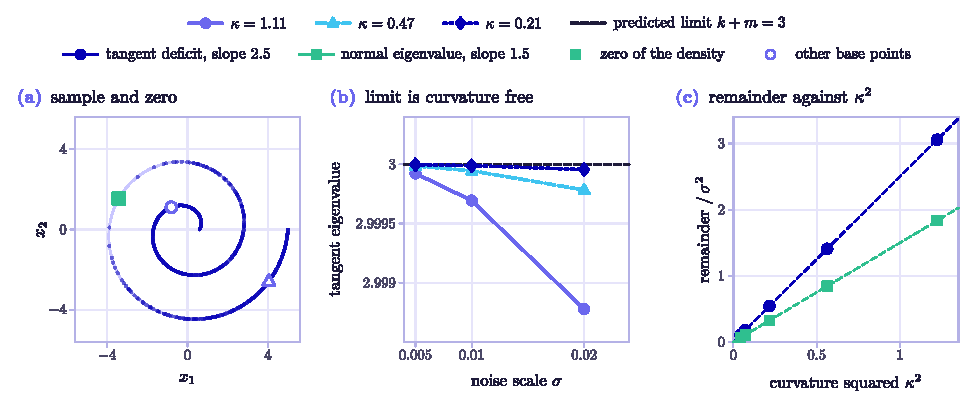
\includegraphics[width=\linewidth]{figures/spiral.pdf}
  \caption{A finite-type zero on a manifold with non-constant curvature.  (a) Fourteen hundred points drawn from the clean density \eqref{eq:spiral-density} for the zero at the filled square, with the manifold itself drawn as a faint guide.  The samples thin to nothing around that point, which is the feature the theorem is about.  The hollow circle and triangle mark two of the other tested base points; each carries its own density vanishing there, so each would empty a different part of the arc.  Both axes use the same scale, so the spiral keeps its true shape.  (b) The tangent Rayleigh quotient against noise scale at the three curvatures given in the legend, all converging to the predicted $k+m=3$ shown dashed, at rates that differ.  (c) The remainder at $\sigma=5\times10^{-3}$ against $\kappa^2$, with the dashed reference lines of slope $2.5$ for the tangent deficit and $1.5$ for the normal eigenvalue.  The limit does not depend on curvature; only the $O(\sigma^2)$ remainder does.}
  \label{fig:spiral}
\end{figure}

\section{Experimental details and numerical checks}
\label{app:experiments}

This appendix records the protocol of the population, finite-sample, and
exact-linearization experiments and of the trained-denoiser and end-to-end
optimization experiments.

\paragraph{Circle quadrature.}
We use a periodic uniform grid of $200{,}001$ points on $[-\pi,\pi)$ for the
spectrum experiment and $120{,}001$ points for each crossover curve.  The
right endpoint is excluded, so the same circle point is not counted twice.
At query angle $\alpha$, unnormalized weights are
\[
  w_j=
  \rho(\theta_j)
  \exp\!\left(
  -\frac{1-\cos(\theta_j-\alpha)}{\sigma^2}
  \right).
\]
After subtracting the largest log-kernel value for numerical stability, the
weights are normalized and the $2\times2$ posterior covariance is computed.
Projecting it onto the tangent and normal vectors at $\alpha$ and
dividing by $\sigma^2$ gives the plotted link blocks.  At the symmetric center
these blocks are eigenvalues.  At a moving query the cross block is generally
nonzero, so Figure~\ref{fig:spatial} labels the tangent quantity as
a Rayleigh quotient.

At the smallest plotted noise $\sigma=0.015$, the tangent eigenvalues for
$r=0,1,2,4$ are respectively
\[
  0.999887,\quad 2.999325,\quad 4.998312,\quad 8.994937,
\]
against predicted limits $1,3,5,9$.  The corresponding normal eigenvalues are at most $1.02\times10^{-3}$.  The same sweep also exhibits the rate in \eqref{eq:hlimit} rather than only its limit.  Regressing $\log|{\lambda_1(H_\sigma)-(k+m)}|$ on $\log\sigma$ over the small-noise end of the grid gives slope $2.000$ for each of $r=0,1,2,4$, and the deviations divided by $\sigma^2$ settle at $0.5000$, $3.0002$, $7.5004$, and $22.5013$.  On this family the observed constants agree with $(m+1)(m+2)/4$ to four digits, with $m=2r$.

\paragraph{Crossover accuracy.}
Across all plotted floor ratios and noise levels, the maximum absolute deviation from
$(\lambda+3/2)/(\lambda+1/2)$ is $3.01\times10^{-2}$ and the median deviation is $3.19\times10^{-3}$.  For the spatial boundary layer, the maximum absolute deviation from
$(a^4+3)/(a^2+1)^2$ is $3.01\times10^{-2}$ and the median is
$2.59\times10^{-3}$.  The largest errors occur at the largest noise, consistent with curvature corrections.

\paragraph{Normal offsets.}
The experiments plotted in Figures~\ref{fig:spatial} and \ref{fig:landing-error} query on the manifold, that is at $b=0$.  To check Theorem~\ref{thm:normal-boundary} at genuinely nonzero normal offset we evaluate the same circle quadrature at
$y=(1+\sigma b)(\cos\sigma a,\sin\sigma a)$, whose rescaled tangential and normal
coordinates are $a$ and $b$.  Table~\ref{tab:normal-offset} reports the tangent
block against its predicted limit $C_a=(a^4+3)/(a^2+1)^2$, the smaller
eigenvalue of $H_\sigma$ divided by $\sigma^2$, and the normal-only landing
error divided by $\sigma^2$.  Three predictions are visible.  The tangent-block
deviation divided by $\sigma$ is constant in $\sigma$, so that block is
$C_a+O(\sigma)$ as stated.  The limit does not depend on $b$: at $a=1$ both
$b=0$ and $b=1.3$ approach $1$, which is the uniformity in the normal
coordinate.  Finally $\lambda_2/\sigma^2$ and the landing error over $\sigma^2$
both converge, confirming $\lambda_{k+1}=O(\sigma^2)$ and the $O(\sigma^2)$
landing bias, and the landing limit does depend on $b$, as
\eqref{eq:normal-boundary-landing} requires through the term
$U_p\{\Lambda_a^\top b-S_ba\}$.

\begin{table}[!htbp]
  \centering
  \caption{Circle quadrature at nonzero normal offset, checking Theorem~\ref{thm:normal-boundary}.  The deviation column is $|U_p^\top H_\sigma U_p-C_a|/\sigma$, which is constant in $\sigma$ when the tangent block is $C_a+O(\sigma)$.}
  \label{tab:normal-offset}
  \small
  \begin{tabular}{@{}rrrrrrr@{}}
    \toprule
    $a$ & $b$ & $\sigma$ & $U_p^\top H_\sigma U_p$ & $C_a$
      & deviation$/\sigma$ & landing$/\sigma^2$ \\
    \midrule
    $0.0$ & $0.0$ & $0.020$ & $2.99880$ & $3.00000$ & $0.060$ & $1.500$ \\
    $0.0$ & $0.0$ & $0.005$ & $2.99992$ & $3.00000$ & $0.015$ & $1.500$ \\
    $1.0$ & $0.0$ & $0.020$ & $0.99967$ & $1.00000$ & $0.017$ & $0.500$ \\
    $1.0$ & $0.0$ & $0.005$ & $0.99998$ & $1.00000$ & $0.004$ & $0.500$ \\
    $1.0$ & $1.3$ & $0.020$ & $0.96200$ & $1.00000$ & $1.900$ & $0.808$ \\
    $1.0$ & $1.3$ & $0.005$ & $0.99031$ & $1.00000$ & $1.937$ & $0.817$ \\
    $-0.8$ & $1.3$ & $0.020$ & $1.21816$ & $1.26770$ & $2.477$ & $0.876$ \\
    $-0.8$ & $1.3$ & $0.005$ & $1.25508$ & $1.26770$ & $2.523$ & $0.898$ \\
    $2.0$ & $-1.1$ & $0.020$ & $0.77537$ & $0.76000$ & $0.769$ & $0.941$ \\
    $2.0$ & $-1.1$ & $0.005$ & $0.76383$ & $0.76000$ & $0.766$ & $0.930$ \\
    \bottomrule
  \end{tabular}
\end{table}

\paragraph{Exact optimization linearization.}
For $C_q=\diag(c,1)$ with $c=m+1$, the four tangent update matrices in
Figure~\ref{fig:conditioning} are
\[
  C_q(I-\gamma C_q),\qquad C_q(I-\gamma I),\qquad
  I-\gamma C_q,\qquad I-\gamma I.
\]
The stable interval of the raw inner-and-outer update is
$((c-1)/c^2,(c+1)/c^2)$ and has width $2/c^2$.  The inner-only interval is
$(1-1/c,1+1/c)$, and the raw-additive interval is $(0,2/c)$; both have width
$2/c$.  The doubly calibrated inner-step-and-normal-only-landing map has
interval $(0,2)$.  The plotted curves are
their exact spectral radii rather than simulated trajectories.  Each method
is evaluated over its own step-size range.

\paragraph{Finite-sample KDE.}
Samples from $\rho(\theta)=(1-\cos\theta)/(2\pi)$ are generated by exact rejection sampling from a uniform proposal, with acceptance probability $(1-\cos\theta)/2$.  For every seed we reuse prefixes of one sample stream at
$N\in\{20{,}000,80{,}000,320{,}000\}$ and evaluate \eqref{eq:empirical-kde} at
$\sigma\in\{0.035,0.05,0.075,0.11,0.16\}$.  We use $48$ fixed consecutive seeds,
$20260819$ through $20260866$.  For each $\sigma$, deterministic quadrature
first computes the finite-noise population reference $H_\sigma$.  We then record
\[
  \|\widehat H_N-H_\sigma\|_\op,\qquad
  \|\mathcal P_1(\widehat H_N)-\mathcal P_1(H_\sigma)\|_\op,\qquad
  |\lambda_1(H_\sigma)-3|,
\]
as separate sampling, subspace, and finite-$\sigma$ quantities.  The exact
population top eigenvalues across the plotted noise levels are respectively
$2.99632,2.99250,2.98310,2.96359,$ and $2.92269$.  Rounded-order success means
$\operatorname{round}(\lambda_1(\widehat H_N)-1)=2$.  Figure~\ref{fig:kde}
shows medians and interquartile ranges for the filled operator-error markers,
median-only open projector-error markers, and Wilson $95\%$ intervals for this
binomial success rate.  Since prefixes from a replication
are nested and effective sample size is itself random, the pooled display is
descriptive; no independence across plotted cells or universal
$\mathrm{ESS}^{-1/2}$ law is claimed.

\paragraph{Learned denoisers.}
Each denoiser is a residual MLP with two tanh hidden layers of
width $96$, and all of its parameters are trained.  Its inputs are the scaled
noisy vector and a normalized
$\log\sigma$ coordinate.  If $r_\theta(y,\sigma)$ is the network output, then
\[
  D_\theta(y,\sigma)=y+\sigma r_\theta(y,\sigma),
  \qquad
  \ell(\theta)=
  \E\left\|r_\theta(Y,\sigma)-\frac{X-Y}{\sigma}\right\|^2.
\]
The three circle noise levels are $0.08,0.12,0.18$, and the plane levels are
$0.12,0.18,0.25$; during training $\sigma$ is drawn uniformly from these three
values rather than from a continuous range, and the same three values are used
for evaluation.  Training pairs are generated afresh at every step from the
exact sampler, so there is no fixed finite training set and no repetition, and
the learned-model error therefore reflects approximation and optimization error
rather than memorization of a sample.  The scaled noisy input is $y$ divided by
$1.25$ for the circles and by $0.85$ for the plane.  We optimize every parameter for $3500$ Adam steps with batch
size $768$, cosine-decayed learning rate from $2.5\times10^{-3}$ to
$2.5\times10^{-4}$, weight decay $2\times10^{-6}$, and gradient-norm clipping
at $8$.  Validation uses $20{,}000$ fresh pairs.

To increase query coverage without changing the population regression
function, each minibatch mixes $15\%$ unweighted samples with $85\%$ samples
resampled from an eight-times-larger pool according to the strictly positive
weight $w(y)=\exp\{-\|y-c\|^2/(2r^2)\}+10^{-4}$, normalized over the pool, which
depends only on $Y$; here $c$ is the evaluation point and $r$ the query radius
below.  Multiplication of the joint density by a
function of $Y$ leaves $\mathbb E[X\mid Y=y]$ unchanged wherever the weight is
positive.  The query radii are $0.22$ for the circle and $0.38$ for the plane.
This resampling changes finite-model optimization but not the population
conditional target.

The residual MLP has an analytic input Jacobian obtained by the chain
rule through both tanh layers.  We form
$\widehat H_\theta=\operatorname{sym}(\nabla_yD_\theta)$, then evaluate the raw
matrix, its hard top-$k$ projector, and $\Phi_{0.25}((\widehat H_\theta)_+)$.
For the regime diagnostic of Table~\ref{tab:calibration-regime} we also record,
in the true tangent frame at the evaluation point, the coupling block
$\|P^\perp\widehat H_\theta P\|_\op$ and the computed separation
$\delta(\widehat H_\theta)$ of \eqref{eq:computed-separation}, obtained from the
two compressions $U^\top\widehat H_\theta U$ and
$U_\perp^\top\widehat H_\theta U_\perp$, where the columns of $U_\perp$ are an
orthonormal basis of the normal space.  A
centered finite-difference audit with step $10^{-6}$ and seed $2026081998$
found an operator-norm Jacobian discrepancy of $1.69\times10^{-10}$.  The plane population reference is evaluated in closed form rather than by
quadrature: homogeneity of $q_4$ makes the tilt scale free, so
$H_\sigma(p)=\tfrac{s^2}{s^2+\sigma^2}UC_qU^\top$ with $s=0.35$ and
$C_q=\diag\{(m+1+\epsilon)/(1+\epsilon),(1+\epsilon(m+1))/(1+\epsilon)\}$ for
$m=4$ and anisotropy $\epsilon=0.1$, whose trace is $k+m=6$.  The fixed
plane frame is obtained by seeded QR in $\R^{16\times2}$.  Its latent
distribution is sampled exactly as a mixture of polynomially tilted
Gaussians; a $4{,}000{,}000$-draw check with seed $2026081997$ obtained second
moments $(0.568106,0.167006)$ against analytic values $(0.567955,0.167045)$, with
maximum relative error $2.67\times10^{-4}$.

There are $12$ independent base replications indexed by seeds $2026081900$
through $2026081911$.  Each replication trains one model for each of the three
problems, for $36$ denoisers total; the plane frame seed is $2026081901$, and the paired
bootstrap seed is $2026081999$.  Shaded figure bands show interquartile ranges,
not confidence intervals.  The two quoted paired intervals use $20{,}000$
percentile-bootstrap resamples of the within-seed raw-minus-hard differences.

\paragraph{Learned optimization.}
For the circle we minimize $f(x)=\|x-(1,0)\|^2/2$ from angle $0.55$ for $35$
steps; for the plane we minimize $f(x)=\|U^\top x\|^2/2$ from latent
coordinate $(0.40,-0.32)$ for $30$ steps.  Both targets are ambient critical
points, as required by Corollary~\ref{cor:local-invariant}.  For each method,
we sweep $20$ circle step sizes from $0.05$ to $1$ and $24$ plane step sizes
from $0.05$ to $1.2$.  Each sweep is run at all three noise levels the
corresponding denoiser was trained on, namely $0.08,0.12,0.18$ for the circle and
$0.12,0.18,0.25$ for the plane, which requires no additional training because the
networks are noise conditional.  Figure~\ref{fig:learned-optimization} plots
the middle level of each problem, $\sigma=0.12$ and $\sigma=0.18$, and the
noise dependence of the achieved floor is reported in
Section~\ref{sec:experiments}.
The raw method uses $\widehat H_\theta$ in the inner step and
$D_\theta$ as the outer landing.  The inner-only method replaces the first by
$\mathcal P_k(\widehat H_\theta)$ but retains raw landing.  SC-DRGD uses the
hard projector in both the tangent step and the normal-only landing.  Oracle
Riemannian gradient descent is included as a deterministic reference.  We
report the projected objective gap
$F(x_t)-F(p)=f(\pi(x_t))-f(p)$ and distance to the manifold for every
iteration, seed, method, and step size; for the affine plane, $F=f$.  Values
are clipped only when drawing the log-scale figure.

\paragraph{Compute.}
The reported run used the full training configuration with Python 3.12.13 and
NumPy 2.3.5 on an arm64 CPU without an accelerator; its recorded
wall-clock time was $169.8$ seconds.


\end{document}
